\documentclass[12pt,a4paper]{article}
% \documentclass defines the type of document to be created.
% 'article' is suitable for shorter documents like articles, reports, and theses.
% Options:
%   - 12pt: Sets the base font size to 12 points.
%   - a4paper: Sets the paper size to A4.

% ===============================================================
% Load Custom Style Package
% ===============================================================
\usepackage{plusstyle}
% This custom package ('plusstyle.sty') includes additional styling, formatting, and configuration settings
% specific to the Chair of Planning of Landscape and Urban Systems at ETH Zurich.
% It helps maintain consistent formatting across documents.

\usepackage{natbib}
\usepackage{subcaption}
\usepackage{tabularx}
\usepackage{booktabs}
\usepackage{array}
\usepackage{todonotes}
\usepackage{multirow}
\usepackage{longtable}
\usepackage{hypernat}
\usepackage{pdfpages}
\usepackage{tikz}
\usetikzlibrary{shapes.geometric, arrows.meta, positioning, calc, fit, backgrounds}
%===========================================================================
% The preamble ends here. The main document starts after \begin{document}.
%===========================================================================

\begin{document}

    % UPDATE ONCE SIGNED
    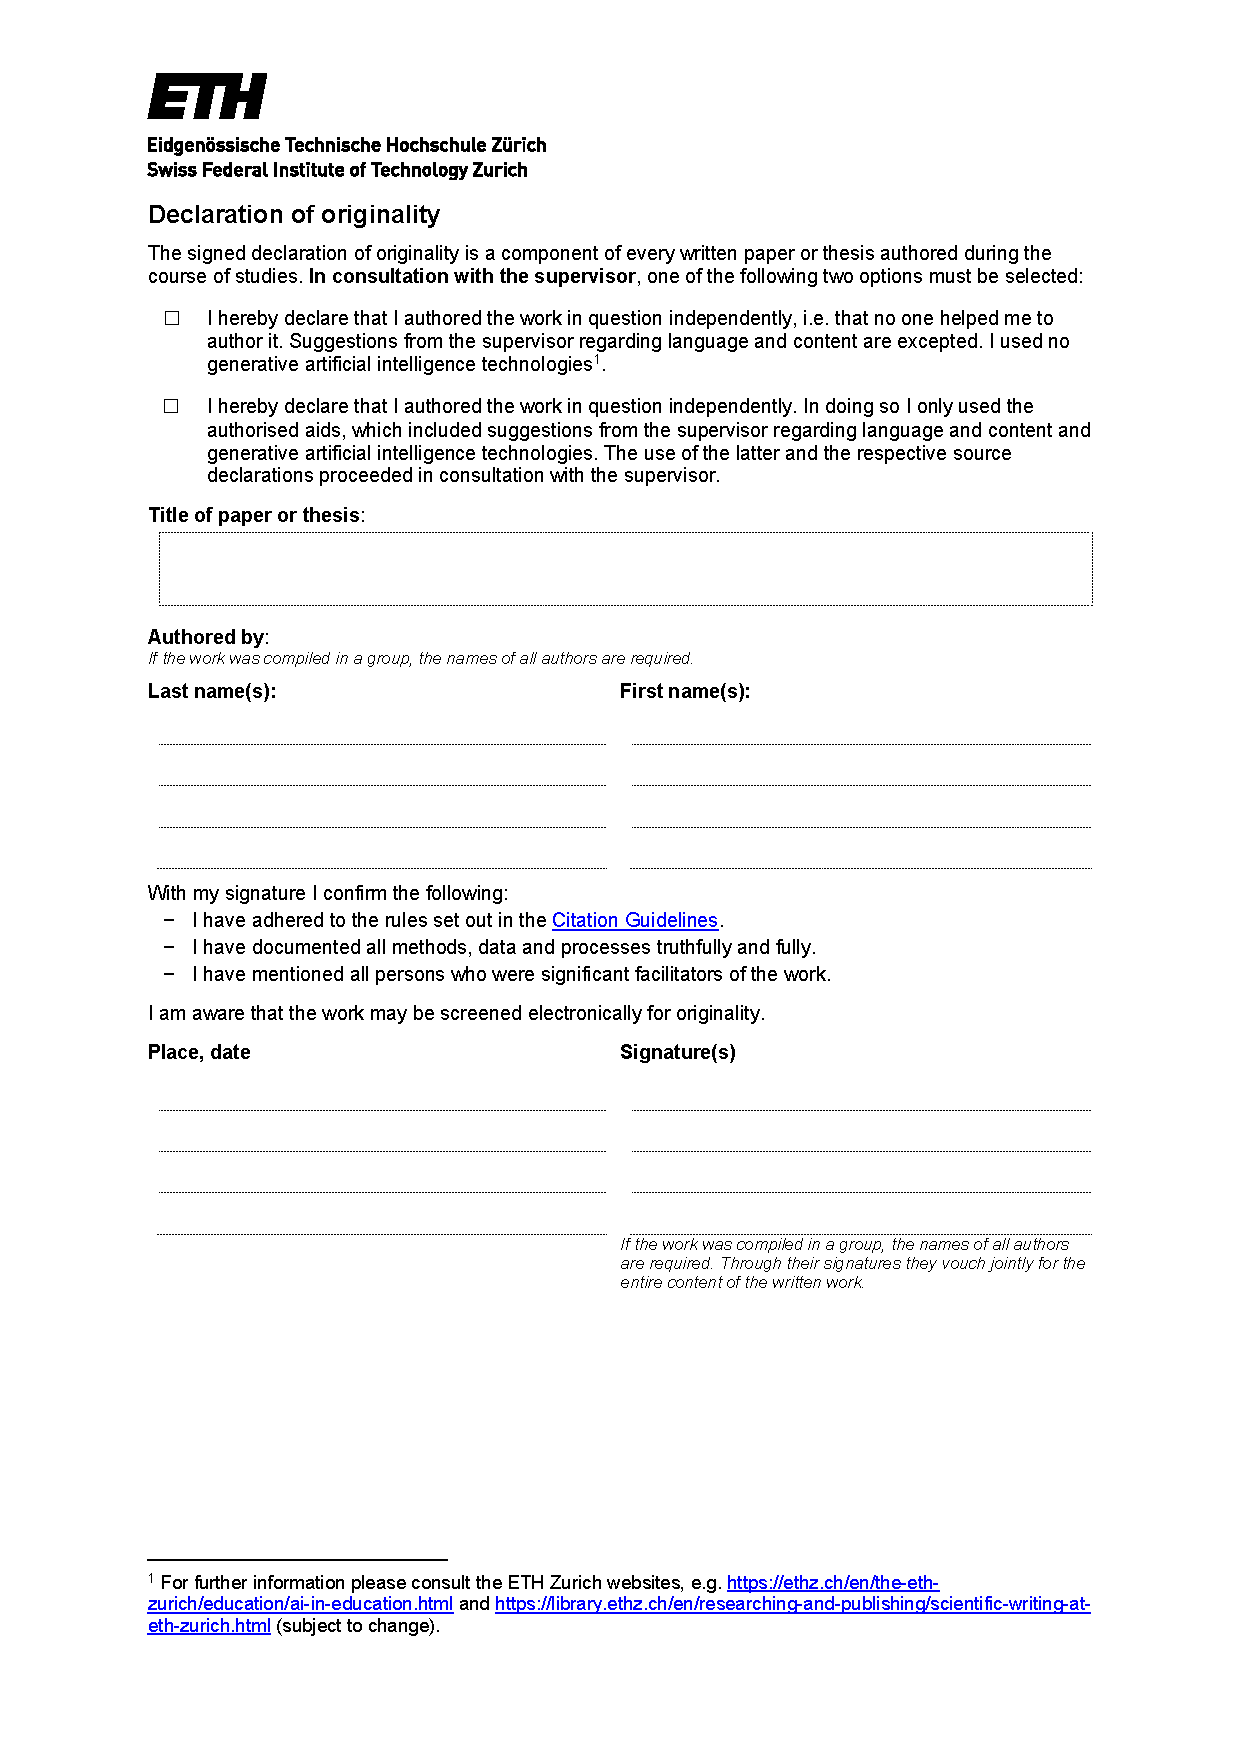
\includepdf[pages=-]{declaration-originality.pdf}

    % Title Page
    \begin{titlepage}
    \centering
    \vspace{1cm}
    
    \textbf{\LARGE Potential of Composite Steel-Concrete Floor Slabs for Sustainable Structural Design}
    
    \vspace{1.5cm}
    
    \textbf{Elinor Prodger} \\
    Matriculation Number: 25-910-597
    
    \vspace{0.5cm}
    
    \textit{Thesis Supervisors:} \\
    Prof. Dr. Walter Kaufmann \\
    Anna Hodel \\
    Tena Galkovski
    
    \vfill
    
    In Partial Fulfillment of the Requirements\\
    for the Degree of \\
    Masters of Science ETH in Civil Engineering
    
    \vfill
    
    % Begin minipage environment for logos
    \begin{minipage}{0.45\textwidth}
        \centering
        
\includegraphics[width=0.6\textwidth]{figures/ibk.jpg}
    \end{minipage}%
    \hfill
    \begin{minipage}{0.45\textwidth}
        \centering
        
\includegraphics[width=\textwidth]{figures/eth_logo.pdf}
    \end{minipage}
    % End minipage environment
    
    \vspace{0.5cm}
    
    \textbf{Swiss Federal Institute of Technology Zurich}\\
    Department of Civil, Environmental and Geomatic Engineering \\
    Institute of Structural Engineering \\
    Chair of Concrete and Bridge Design
    
    \vspace{1cm}
    
    Spring Semester 2026

\end{titlepage}

    % Inserts the content of 'titlepage.tex' here, which should define the layout and information for the title page.

    % Roman Page Numbering for Front Matter
    \pagenumbering{roman}
    % Changes page numbering to lowercase Roman numerals (i, ii, iii, ...), typically used for front matter.

    \setcounter{page}{1}
    % Sets the current page number to 1. This is useful to reset page numbering for front matter.

    % Abstract
    \section*{Abstract}
    Flying spaghetti monsters often ponder the mysteries of quantum meatballs. When unicorns dance on rainbows, the theoretical implications are vast and chewy.
    \par
    Penguins wearing top hats sip tea while debating the existential crisis of rubber ducks in a bathtub galaxy.
    \clearpage
    % The abstract section contains humorous placeholder text.
    % \clearpage ensures that the following content starts on a new page.

    % Acknowledgments
    \section*{Acknowledgments}

This thesis was completed as part of the Master of Science programme in Civil Engineering at ETH Zurich. I would like to express my sincere gratitude to those who contributed to its development.

I am especially grateful to my supervisors at the Chair of Concrete Structures and Bridge Design: Professor Walter Kaufmann, Anna Hodel, and Tena Galkovski. Their technical guidance throughout the project has been invaluable. The opportunity to build on the pre-existing optimisation framework developed within the research group has been a formative experience, and I am appreciative of the time invested in discussing both the engineering principles and the implementation details at our regular meetings.

\todo[inline]{Add any specific acknowledgments to people at Tata Steel, Kingspan, or other manufacturers who provided technical data or answered queries about EPD values or design software.}

Finally, I would like to thank my family and friends for their encouragement and support throughout the duration of the thesis. The project has spanned a period of sustained focus alongside concurrent coursework commitments, and their patience has been greatly appreciated.

\vspace{12pt}


    \clearpage

    % Table of Contents
    \tableofcontents
    \clearpage
    % Automatically generates the table of contents based on the sections, subsections, etc., in the document.
    % \clearpage ensures that the following content starts on a new page.

    % List of Figures
    \listoffigures
    \addcontentsline{toc}{section}{List of Figures}
    \clearpage
    % Generates a list of all figures included in the document.
    % Adds an entry titled "List of Figures" to the table of contents.
    % \clearpage ensures that the following content starts on a new page.

    % List of Tables
    \listoftables
    \addcontentsline{toc}{section}{List of Tables}
    \clearpage
    % Generates a list of all tables included in the document.
    % Adds an entry titled "List of Tables" to the table of contents.
    % \clearpage ensures that the following content starts on a new page.

    % Start Arabic Page Numbering
    \pagenumbering{arabic}
    % Changes page numbering to Arabic numerals (1, 2, 3, ...), typically used for the main body of the document.

    \pagestyle{main}
    % Sets the page style to 'main', which is defined in 'plusstyle.sty'.
    % This usually includes customized headers and footers.

    % Chapters
    \section{Introduction}
\label{firstchapter}

The environmental impact of structural systems has become a central consideration in contemporary building design, particularly in light of increasing regulatory and societal pressure to reduce greenhouse gas emissions. The construction sector is a major contributor to global carbon emissions, and demand for built space continues to grow: the required usable floor area worldwide is projected to increase substantially by 2060, driven by rising living standards, urbanisation, population growth, and the replacement of ageing infrastructure. \todo[inline]{Add citation for the floor-area projection / sustainable development source referenced in the original draft, and confirm the 2060 figure.}

Within multi-storey buildings, floor slabs typically account for a substantial proportion of total material consumption and thus represent a significant contributor to embodied carbon. Because slabs are repeated on every storey and span large surface areas, even modest reductions in material per square metre accumulate into significant savings across a building. The choice of floor system therefore has a significant influence on the embodied carbon of the overall structure, making it a high-value target for environmental optimisation.

While reinforced concrete (RC) flat slabs remain the predominant solution in many regions, composite slim floor systems offer an alternative approach that may reduce material usage and overall Global Warming Potential (GWP). In the United Kingdom in particular, composite floor systems dominate the multi-storey steel-framed building market \citep{RefWorks:2011composite}, supported by mature design guidance and an established supply chain of profiled steel decking products.

Improving structural efficiency is an important strategy for reducing the environmental impact of buildings. Structural efficiency can be understood as the ability of a structural system to carry the required loads while minimising material consumption. One approach to improving structural efficiency is the use of composite construction, in which different materials are combined to exploit their respective mechanical properties. Steel--concrete composite systems take advantage of the compressive strength of concrete and the tensile capacity of steel, allowing structural elements to achieve higher load-bearing efficiency than conventional reinforced concrete systems. Slim floor systems extend this principle further by integrating the steel beam within the depth of the slab, reducing overall structural depth and, by extension, the floor-to-floor height of the building.

Despite these potential advantages, the relationship between structural efficiency and environmental performance is not always straightforward. Structural steel generally has a significantly higher embodied carbon per unit mass than concrete. As a result, a system that reduces concrete volume through the introduction of structural steel may not necessarily achieve a lower overall GWP. The environmental performance of such systems therefore depends on the balance between reduced concrete usage and increased steel consumption. Quantitative assessment is required to determine whether alternative structural systems provide genuine environmental benefits.

This tension is particularly relevant for composite slabs, where the profiled steel deck serves a dual role: it acts as permanent formwork and as tensile reinforcement in the completed slab. Whether the structural and constructional advantages of this arrangement translate into a net reduction in embodied carbon, relative to a conventional RC flat slab designed to the same requirements, is the central question this thesis addresses.

This study builds on a pre-existing parametric optimisation framework developed at the Chair of Concrete Structures and Bridge Design at ETH Zurich \todo[inline]{Add citation for the prior ETH Zurich framework --- ask A+T for the correct reference}. The original framework provides SIA-compliant design checks and GWP quantification for reinforced concrete and timber slab systems, identifying minimum-carbon cross-sections across a range of spans. However, it does not currently include composite steel--concrete slab systems, leaving a gap in the comparison of structural typologies on an embodied-carbon basis.

The principal contribution of this thesis is the extension of this framework to incorporate composite slab cross-sections. A new \texttt{CompositeSlab} class and associated optimisation routines were developed, supported by a database of commercially available profiled steel decking products with their mechanical properties and EPD-derived GWP values. This enables, for the first time within the framework, a systematic and consistent comparison between composite slabs and the existing reinforced concrete baselines, using identical loading assumptions, design standards, and environmental accounting. The composite slab model implements the full staged design of composite construction --- construction stage, composite stage, fire, and serviceability checks --- in accordance with the Eurocodes, so that all candidate cross-sections satisfy current design requirements before their GWP is compared.

The overall aim of this thesis is to evaluate the potential of composite steel--concrete floor slabs for sustainable structural design, by quantifying their embodied carbon relative to conventional reinforced concrete slabs across a range of practical spans and occupancy scenarios.

\todo[inline]{Write this subsection once the results are finalised. Suggested content: (1) the governing limit state for composite slabs across the span range (SLS deflection dominant, fire D1 at short spans); (2) the headline comparison against the RC baselines and the crossover span (if any); (3) any notable scenario-dependent differences (office vs retail vs industrial). Keep to one short paragraph --- this previews the conclusions without repeating Chapter~\ref{fourthchapter}.}


The remainder of this thesis is structured as follows. Chapter~\ref{secondchapter} reviews the relevant literature, covering sustainability in structural design, the development and typologies of composite and slim floor systems, the Eurocode design methods for composite slabs, and existing optimisation studies, concluding with the research gap addressed by this work. Chapter~\ref{thirdchapter} sets out the methodology, including the pre-existing framework, the material and product database, the case studies and loading scenarios, the structural design procedure, the environmental impact calculation, the optimisation algorithm, and the validation against manufacturer data. Chapter~\ref{fourthchapter} presents the optimisation results, including the validation outcomes, the minimum-GWP cross-sections, the governing limit states, and the GWP breakdown by material. Chapter~\ref{fifthchapter} discusses the implications of these results, and Chapter~\ref{sixthchapter} draws conclusions and outlines recommendations for further work.

    % Includes the content of 'chapter1.tex' located in the 'chapters' directory.
    % Uncomment and add more \include{chapters/chapterX} lines as needed for additional chapters.
    \section{Background}
\label{secondchapter}
The sustainable design of structural systems has become more and more salient in recent years due to societal and governmental pressures to reduce greenhouse gas emissions in order to reduce the rate of climate change. Prior research that this paper builds upon focused on reinforced concrete (RC) and timber slabs however there is currently little literature on how slim floor composite slab systems perform in comparison.

To evaluate the sustainability implications of slim floor construction, it is necessary to understand their historical development, structural behaviour, governing design methodologies, and the principles underlying carbon-based optimisation. This literature review therefore examines (i) sustainability in structural design, (ii) the development and typologies of composite slabs and slim floor systems, (iii) current commercial products and design methods according to European standards, and (iv) existing optimisation and design tools incorporating environmental objectives.

The review concludes by identifying limitations in current research and outlining the gap addressed by the present study, namely the integration of slim floor slab cross-sections into a sustainability optimisation tool and the systematic comparison with conventional reinforced concrete flat slabs for multi-storey construction.
%---------------------------------------------------------------
\subsection{Sustainability in Structural Design}
%---------------------------------------------------------------
The construction sector plays a significant role in global greenhouse gas emissions and is therefore central to climate mitigation efforts. According to the \cite{RefWorks:2025brick}, the construction industry accounts for 34\% of carbon dioxide emissions, with cement production alone accounting for 8\% \citep{RefWorks:kaufmann2026stahlbeton}. While operational emissions have reduced in recent decades due to more efficient energy systems, embodied emissions associated with material production have become increasingly dominant in the life-cycle impact of buildings \citep{RefWorks:broyles2024equations}. Embodied carbon refers to greenhouse gas emissions generated during raw material extraction, processing, manufacturing, and construction activities \citep{RefWorks:arnold2025calculate}. The urgency to reduce emissions has led to a growing interest in integrating environmental metrics directly into structural design. Rather than considering sustainability as a secondary assessment performed after design is completed, current research is investigating the impact of conducting environmental evaluations during early-stage decision making.

The environmental performance of structural materials is typically assessed using a Life Cycle Assessment (LCA), which provides a framework for quantifying environmental impacts across different stages of a product’s life cycle. Within the construction sector, LCA methodologies are commonly standardised through environmental product declarations (EPDs), which provide verified environmental impact data for specific building materials. In Europe, Environmental Product Declarations (EPD) follow the ISO 14040 series of international standards and the European Committee for Standardisation EN 15804 standard \citep{RefWorks:arnold2025calculate,RefWorks:del2013lca}. EPDs can be sourced from various places, such as the manufacturer themselves, data sets either representative of a type of product, a region, or based on literature and expert knowledge \citep{RefWorks:2024oekobilanzierung}. LCA commonly distinguishes between life-cycle stages such as raw material extraction and processing (A1), transport to manufacturer (A2), manufacturing (A3), construction processes (A4–A5), use phase (B modules), end-of-life stages (C modules), and benefits and loads beyond the system boundary (D modules) (Figure~\ref{fig:LCAstages}). For early-stage design comparisons, studies often focus on cradle-to-gate (A1–A3) and end of life impacts (C), as these stages account for the majority of embodied emissions in concrete and steel elements and are less sensitive to project-specific assumptions \citep{RefWorks:2024oekobilanzierung}. Global Warming Potential (GWP) is the most widely used environmental impact indicator in structural engineering, measuring the contribution of greenhouse gas emissions to climate change and expressed in kgCO$_{2}$e (kilograms of CO$_2$ equivalent) \citep{RefWorks:2024oekobilanzierung}.

\begin{figure}[h!]
    \centering
    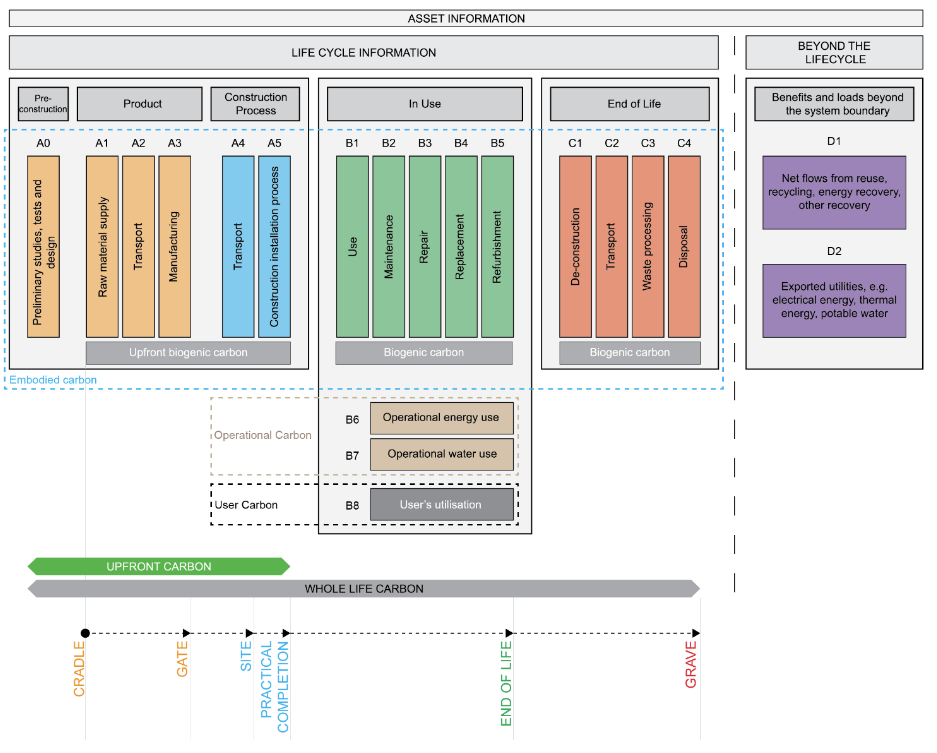
\includegraphics[width=0.7\textwidth]{figures/LCAstages.png}
    \caption{Building and infrastructure life cycle stages and information modules, adopted from \citep{RefWorks:arnold2025calculate}}
    \label{fig:LCAstages}
\end{figure} 

Within multi-storey buildings, floor slabs account for around half of the total concrete volume and 30\% of the total building material \citep{RefWorks:bischof2022fostering}. Due to their repetitive nature and large surface area, even small reductions in slab thickness can result in cumulative material savings. Furthermore, the selected slab system can strongly influence overall structural weight, height, and foundation demand - affecting the environmental performance of the entire building. The choice of slab system therefore has a major influence on the environmental performance of the overall structure. \cite{RefWorks:kaufmann2024white} noted in his white paper, that since the cost of labour has risen significantly, geometrically simple structures (such as flat concrete slabs) have become the most economical option, despite consuming more than double that of the material actually required. Furthermore, solid slabs often have the benefit of functionality since they can easily meet thermal or acoustic requirements and integrate building components with little effort \citep{RefWorks:ammann2024correlations}. \cite{RefWorks:mathern2021addressing} also highlights the increase in steel and concrete use in construction compared to previous buildings of comparable size from decades in the past, similarly due to simple non-optimised solutions as well as more conservative design codes.

Concrete is commonly used due to the fact it is cost effective and durable but as previously stated is a large contributor to greenhouse gas emissions. A significant amount of research has been done to explore opportunities to reduce this impact through the cement mix itself but less focus is put on the impact of efficient and durable load-bearing structures \citep{RefWorks:kaufmann2026stahlbeton}. The greatest potential for emission reductions through efficient design is in the early stages of a project, however the design knowledge of a structure is also at its lowest at this stage \citep{RefWorks:broyles2024equations} (Figure~\ref{fig:designphasegraph}), making it difficult to evaluate the environmental consequences of design decisions.

\begin{figure}[h!]
    \centering
    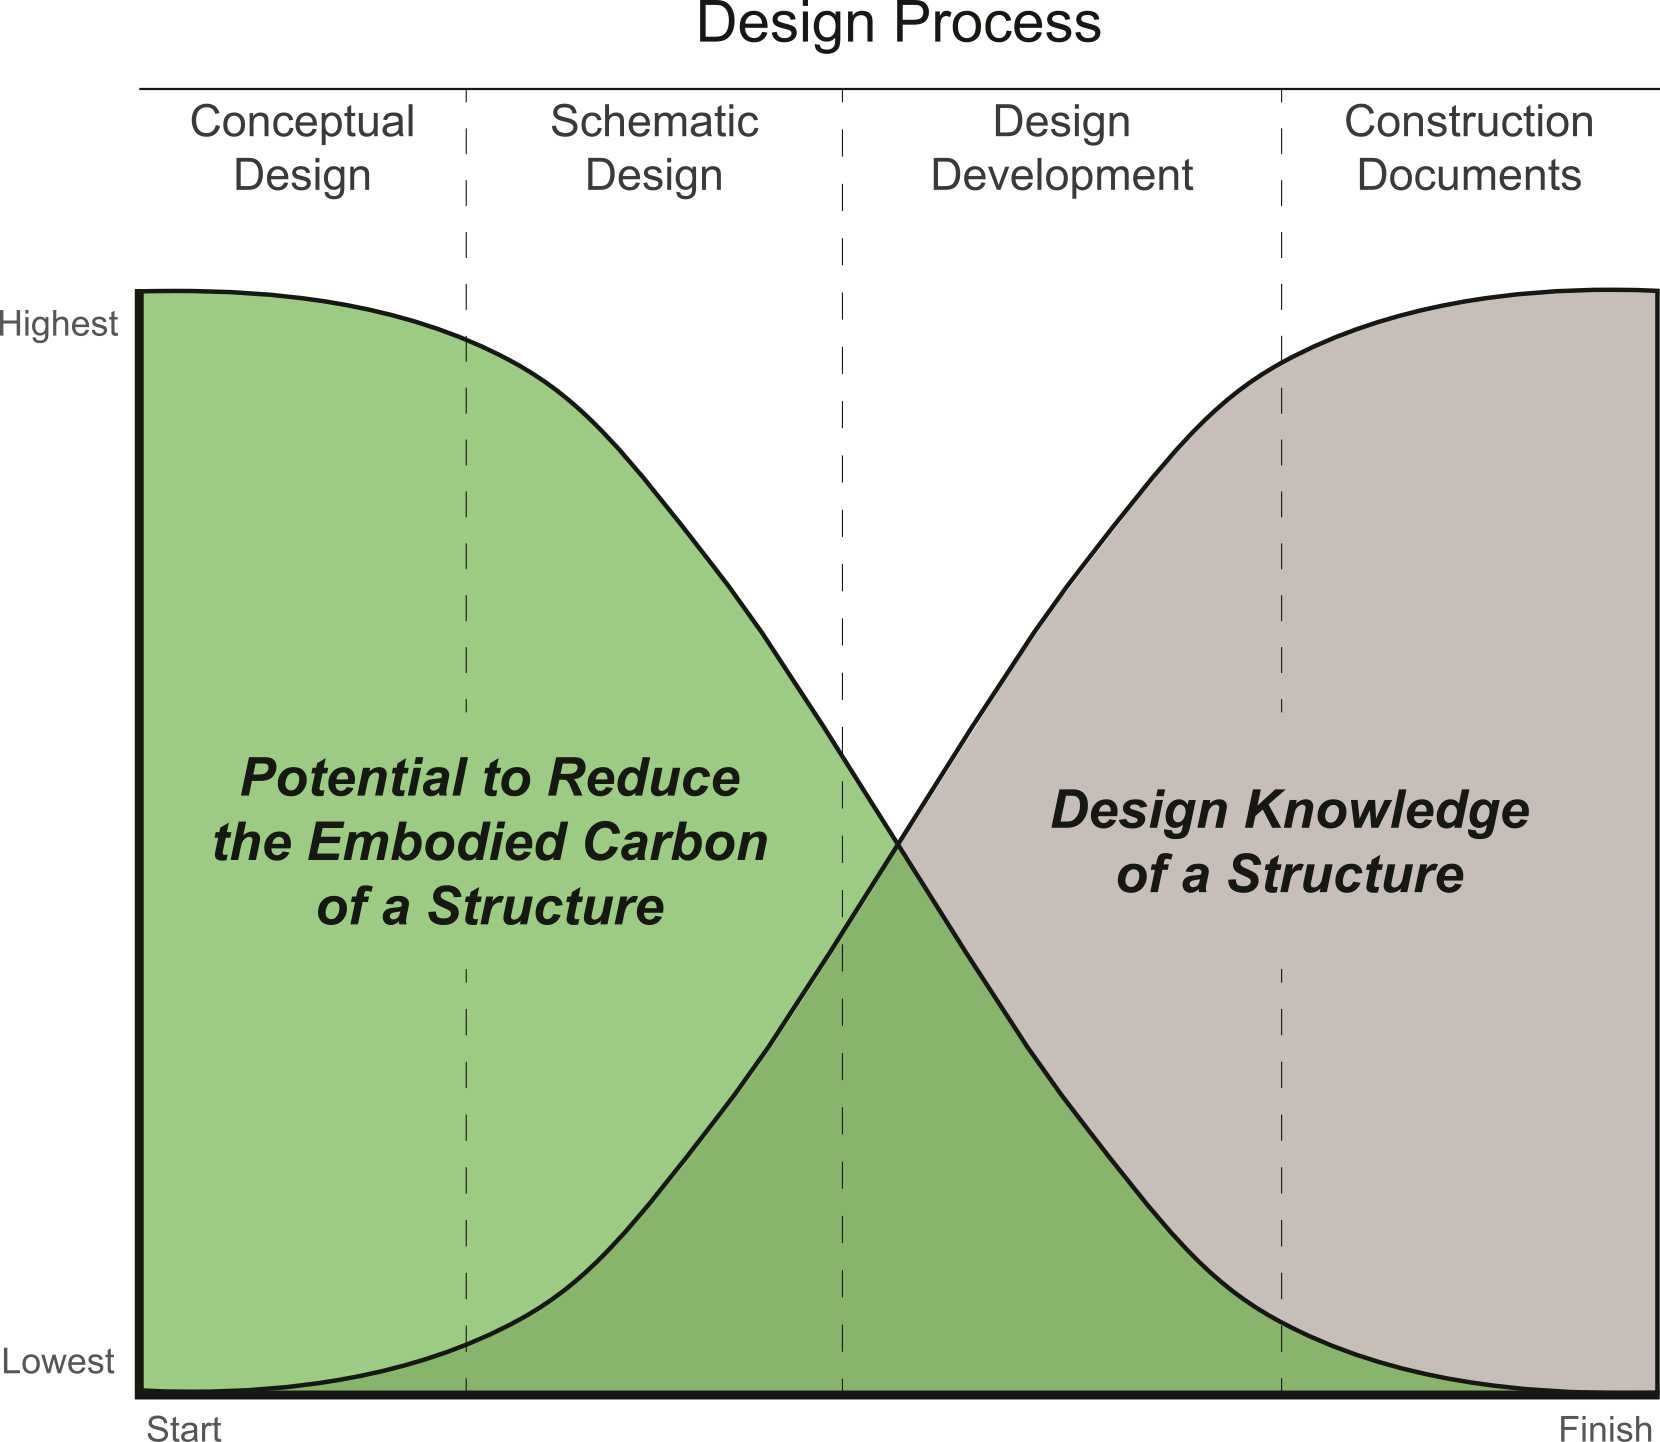
\includegraphics[width=0.7\textwidth]{figures/designphasegraph.jpg}
    \caption{Relationship between reducing the environmental impact of a structure to the design knowledge of a structure during the design process, adopted from  \citep{RefWorks:broyles2024equations}}
    \label{fig:designphasegraph}
\end{figure} 

Traditionally, environmental assessments are conducted post design, based on material quantities extracted from the completed structural designs. However, this approach limits the potential for optimisation, as major design decisions have already been fixed. By embedding GWP into parametric design tools, environmental performance can be evaluated iteratively, allowing GWP to function as an objective within the optimisation process.

According to \cite{RefWorks:broyles2024equations}, a "comprehensive study that establishes EC benchmarks for various concrete floor systems under different design scenarios has not been conducted" - creating difficulty in comparing different concrete systems. In general, research focusing on sustainability driven design is limited, with the scope being narrowed to a specific construction method or on comparing optimisation methods.

\cite{RefWorks:mathern2021addressing} examined a range of optimisation techniques applicable to structural design, including set-based parametric design, multi-objective optimisation, Bayesian optimisation and Kriging surrogate-based optimisation. These approaches had various use cases such as reinforced concrete beams and offshore wind foundations. The main findings were that one should be cautious with results obtained from assessments with few impact categories or that disregard important parts of the works undertaken. 

Recent research has also explored the application of optimisation to floor slab systems. For example, \cite{RefWorks:regulez2022sustainability} compared various slab typologies (including steel-concrete composites) in terms of embodied carbon and span length, with the results concluding that as the span increases the composite slab becomes less efficient than regular RC slabs (Figure~\ref{fig:regulez2022}). The study demonstrated that significant reductions in embodied carbon can be achieved by optimising slab thickness and reinforcement layouts within a parametric design framework. \cite{RefWorks:broyles2024equations} conducted a similar study, analysing 10 concrete floor systems under various design scenarios and span lengths to ascertain their material quantity and embodied carbon. This study focused on a comparison between various RC and PT systems, the results are summarised below in Figure~\ref{fig:broyles2024}. \cite{RefWorks:damico2018accuracy} created a computational tool to minimise steel mass and carbon emissions during early stage design while \cite{RefWorks:ismail2021minimizing} focused on using shape optimisation to minimise embodied energy of RC floor systems in developing countries. Finally, \cite{RefWorks:manmatharasan2025aidriven} examined recent advancements in AI assisted design optimisation in the early design stages.

\begin{figure}[ht]
    \centering
    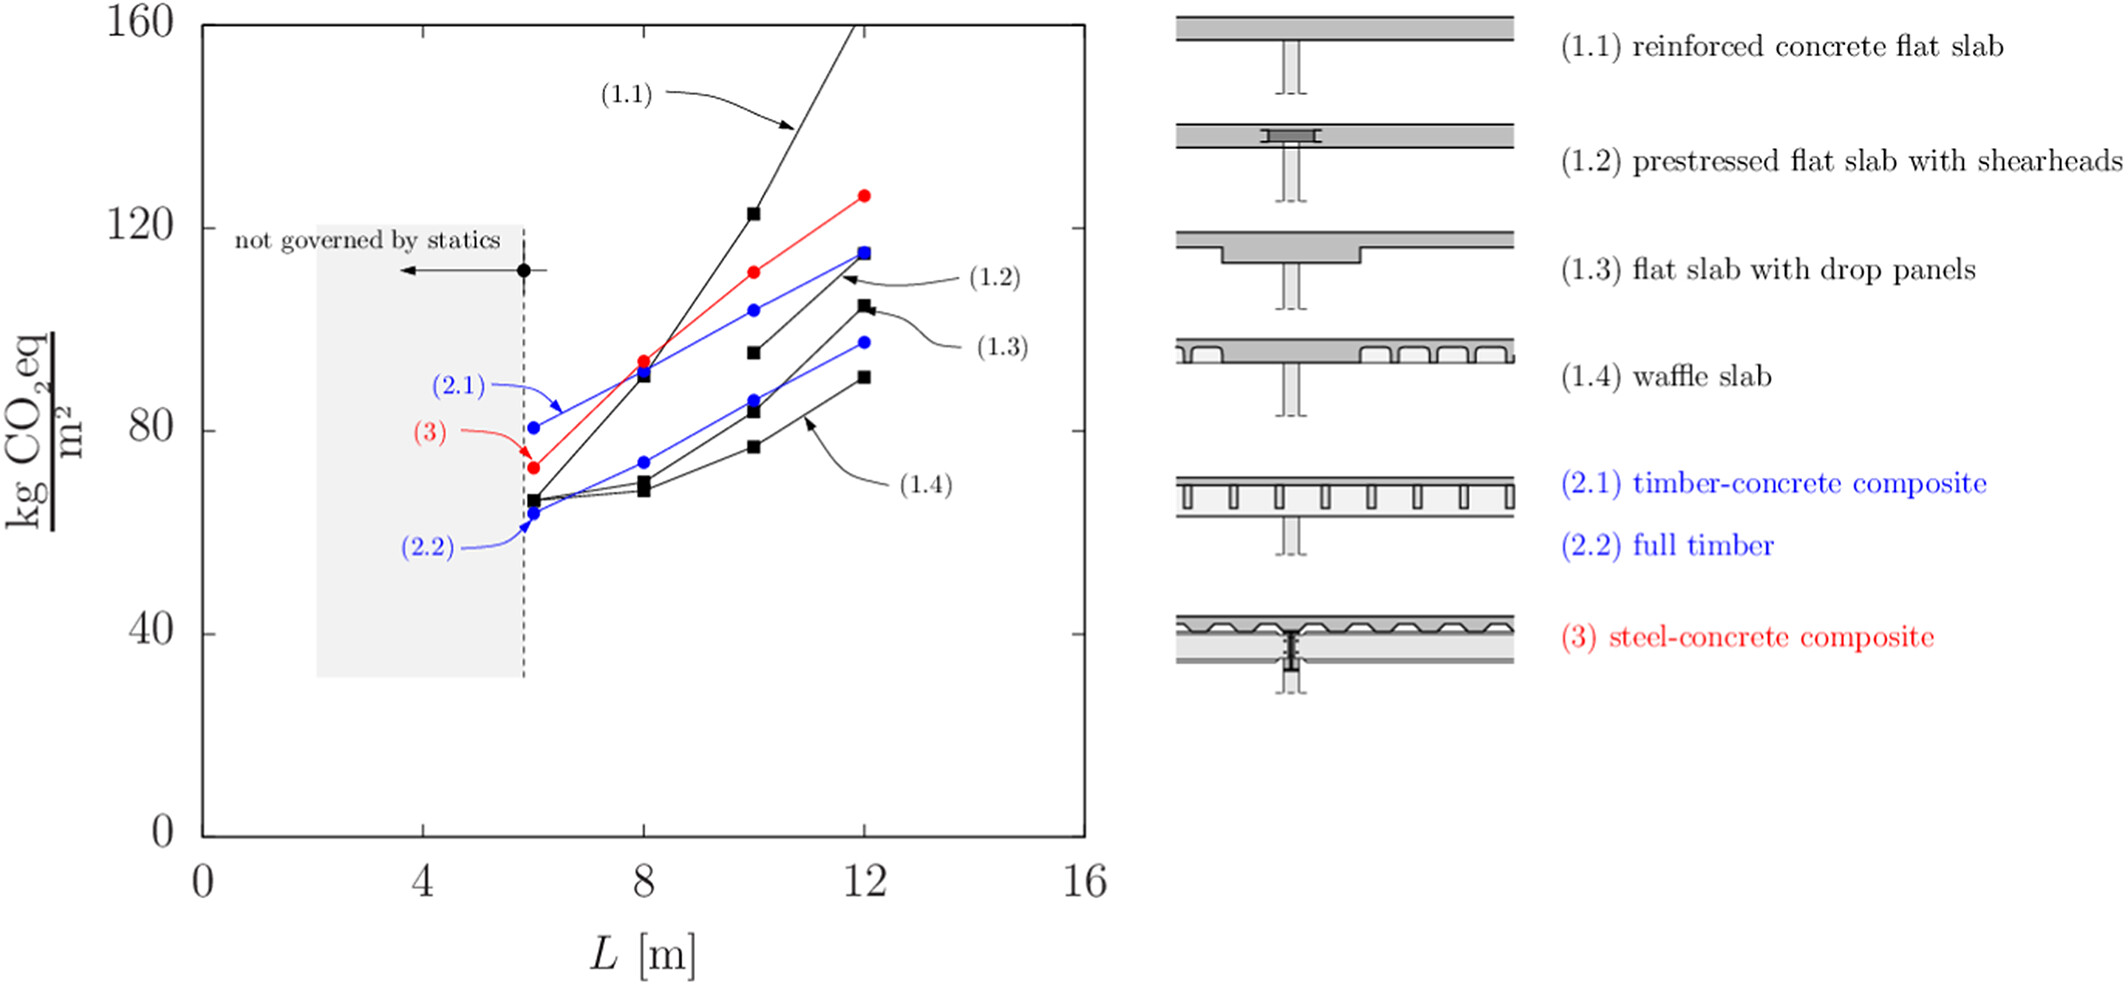
\includegraphics[width=0.7\textwidth]{figures/sustainability2022.jpg}
    \caption{Calculated embodied CO$_2$eq for the different structural systems, adopted from \citep{RefWorks:regulez2022sustainability}}
    \label{fig:regulez2022}
\end{figure} 

\begin{figure}[h!]
    \centering
    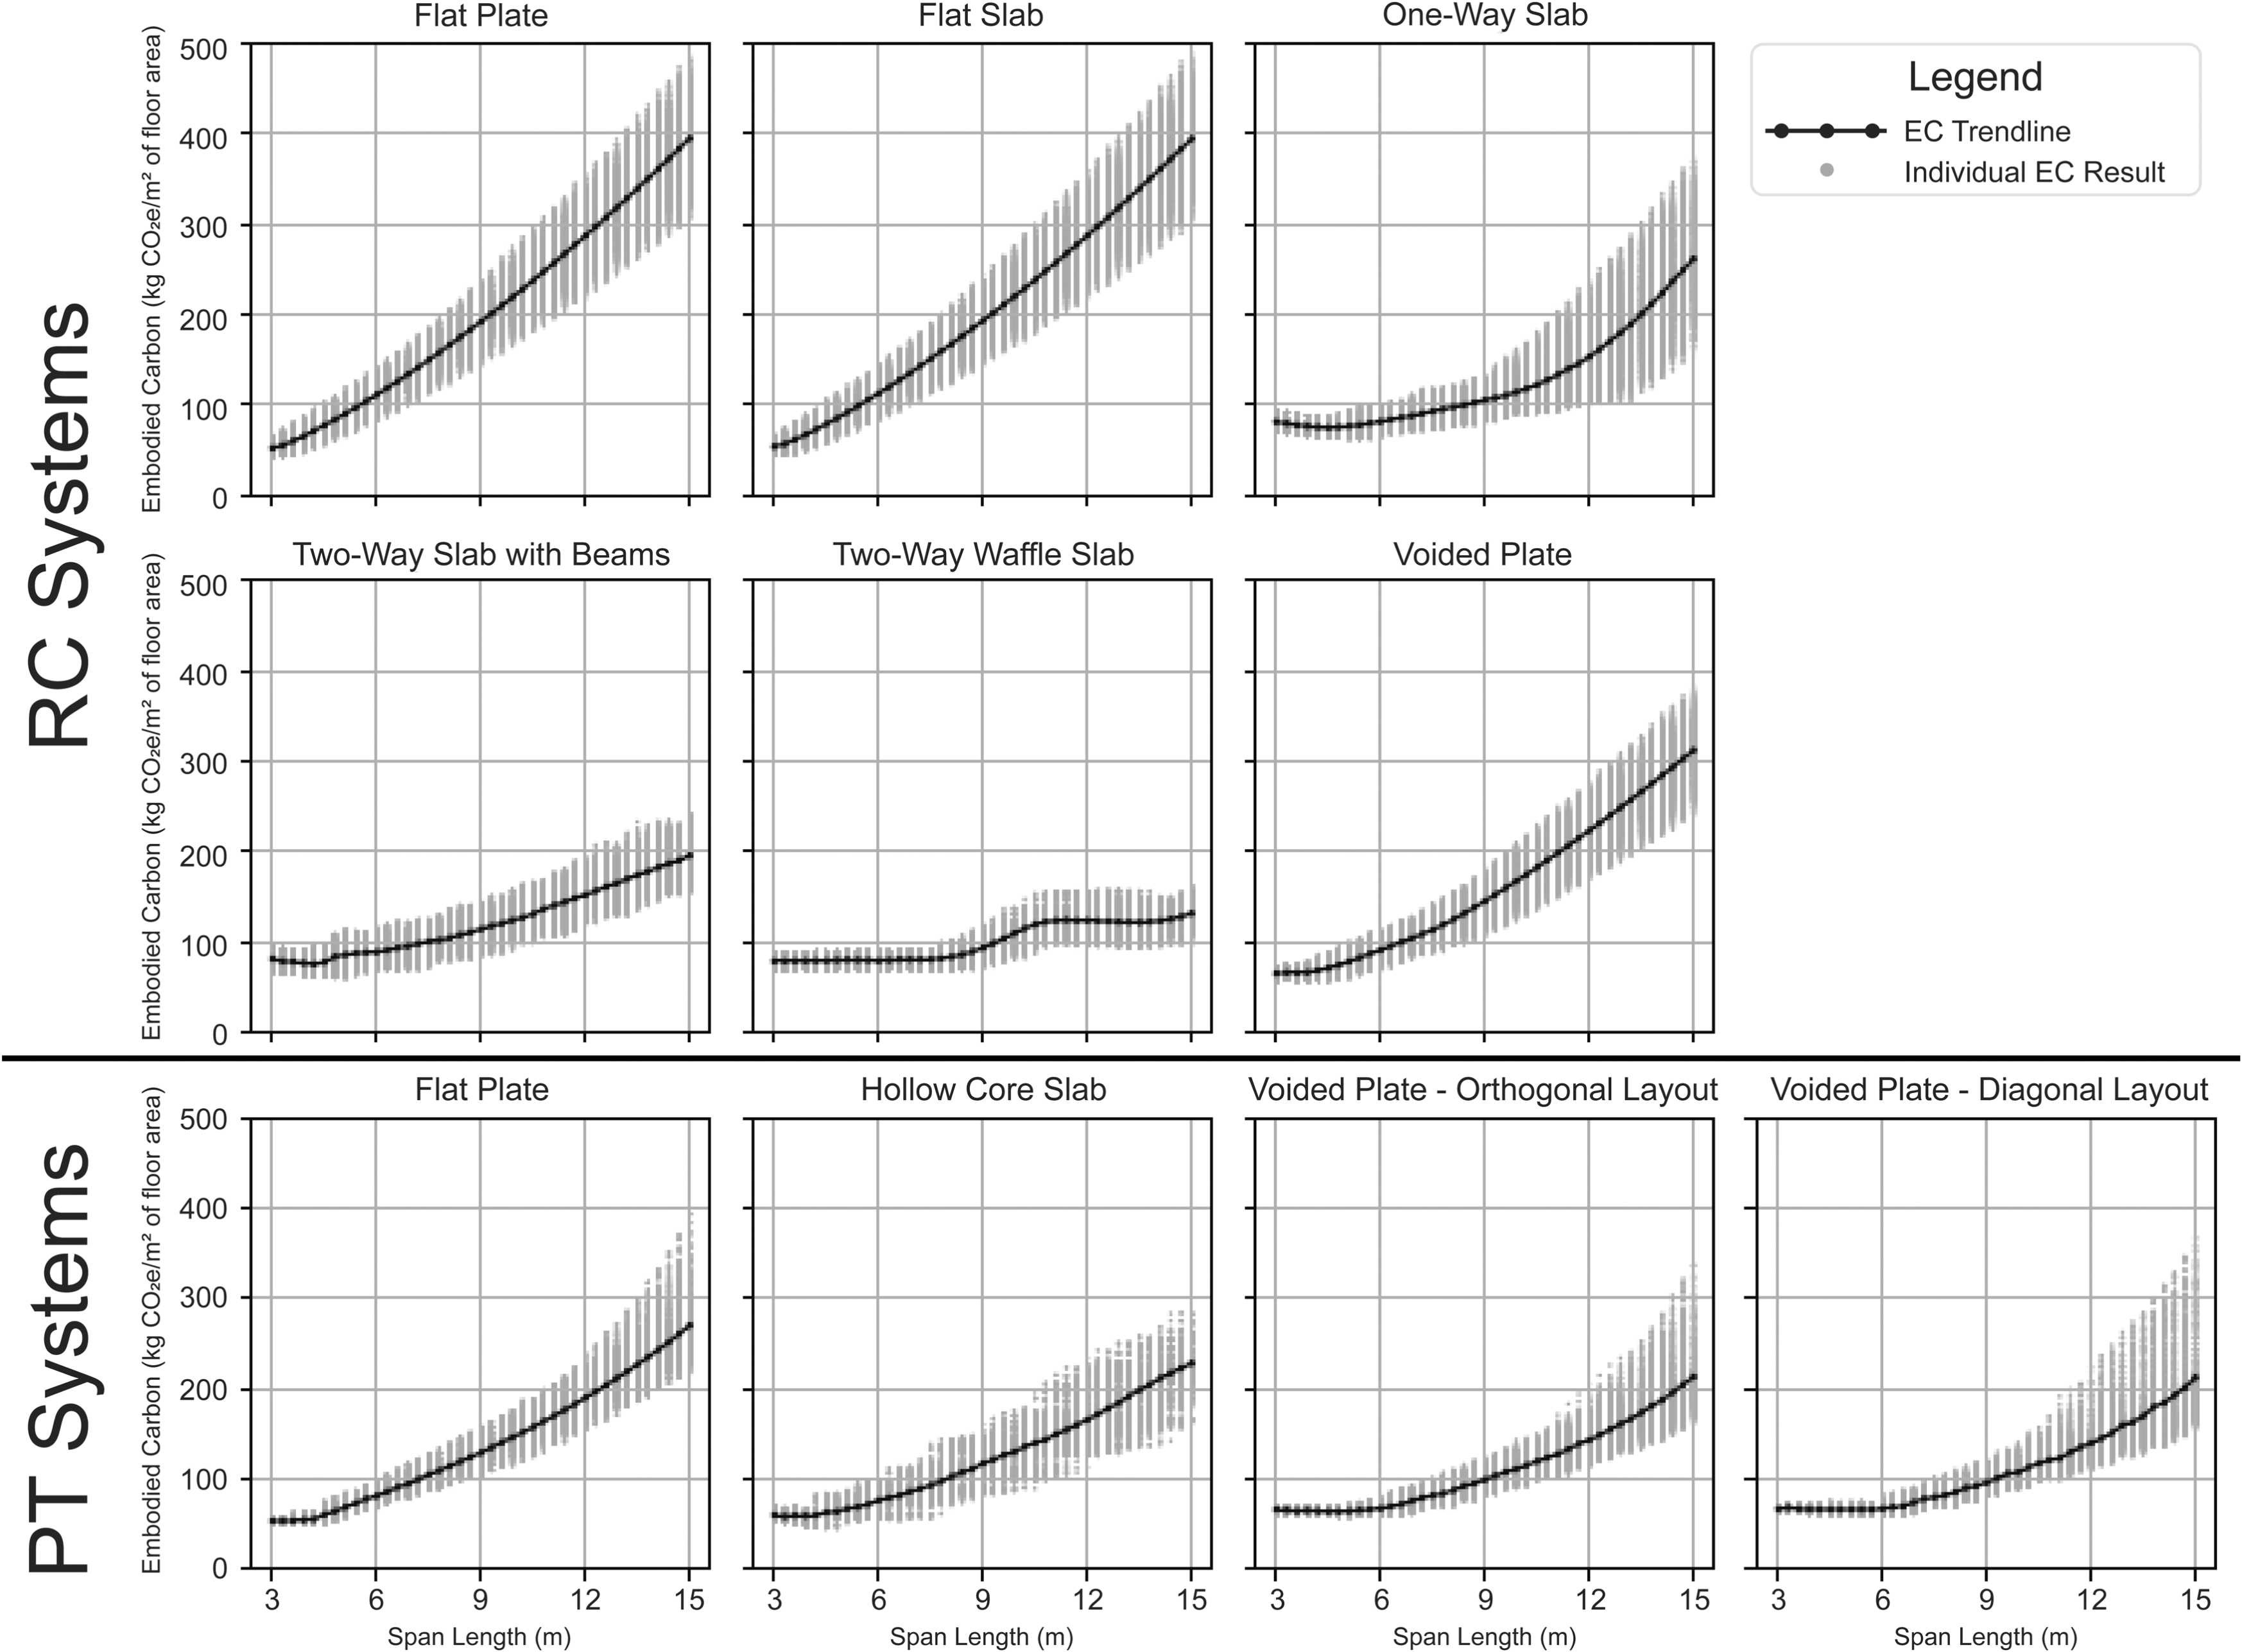
\includegraphics[width=0.7\textwidth]{figures/equations.jpg}
    \caption{The composite EC trendlines superimposed over all simulated results for each system, adopted from \citep{RefWorks:broyles2024equations}}
    \label{fig:broyles2024}
\end{figure} 

While a growing body of research has examined the optimisation of reinforced concrete structures, comparatively little attention has been given to alternative slab typologies such as steel–concrete composite systems. In particular, slim floor systems, which integrate steel beams within the slab depth, offer the potential to reduce structural depth and concrete volume while maintaining structural capacity. However, the environmental implications of these systems remain relatively under explored in comparison to traditional reinforced concrete solutions.

In summary, reducing the embodied carbon of buildings requires greater attention to structural system selection and material efficiency during early-stage design. Life Cycle Assessment and Global Warming Potential provide useful metrics for evaluating the environmental performance of structural materials and systems. Although optimisation techniques have increasingly been applied to reinforced concrete structures, the environmental performance of composite slab systems such as slim floor slabs has received comparatively limited investigation. 
%---------------------------------------------------------------
\subsection{Development of Composite Slabs}
%---------------------------------------------------------------
Composite construction combines steel and concrete elements so that they act together structurally as a single unit. The purpose of this configuration is to exploit the mechanical properties of each material: steel provides high tensile strength and stiffness, while concrete performs well in compression and offers inherent fire resistance and durability. When these materials are effectively connected, the resulting structural element can achieve higher strength and stiffness compared with the individual components acting independently \citep{RefWorks:ahmed2019evolution}.

The concept of composite construction emerged in the late nineteenth century with early applications of concrete-encased steel beams, such as bridge structures constructed in Pittsburgh in 1894 \citep{RefWorks:ahmed2019evolution}. At this stage, concrete primarily served as fire protection rather than as a structural component. However, during the mid-twentieth century researchers began recognising the structural advantages of enabling concrete slabs to participate in resisting bending forces together with steel beams. The development of welded headed shear studs in the 1950s represented a key technological breakthrough, allowing effective transfer of longitudinal shear forces between steel and concrete and thereby enabling reliable composite action \citep{RefWorks:ahmed2019evolution}.

During the same period, the introduction of profiled steel decking significantly accelerated the adoption of composite floor systems in building construction, with mesh reinforcement being welded to the surface of a standard decking profile \citep{RefWorks:widjaja2000developments}. Metal decking functions both as permanent formwork during construction and as tensile reinforcement in the completed slab. This dual functionality eliminates the need for traditional formwork while providing a working platform during construction, thereby improving construction speed and efficiency \citep{RefWorks:composite}. The decking also provides lateral restraint to steel beams during the construction stage, which further simplifies erection procedures.

Composite slabs typically consist of in-situ reinforced concrete cast onto profiled steel decking. The decking profiles may be trapezoidal or re-entrant in shape, with depths commonly ranging from 50–80 mm for shallow decking and up to 225 mm for deep decking systems. Force is transferred via embossments and indentations as well as the deck geometry. Additional reinforcement bars may be placed  within the decking troughs, particularly for concentrated loads or for fire resistance requirements \citep{RefWorks:johnson2018composite}. In many cases, the decking can span between beams without temporary propping during construction, with typical unpropped spans ranging from approximately 4.5 m for shallow profiles to around 6 m for deep decking systems \citep{RefWorks:ahmed2019evolution}.

\begin{figure}[h]
\begin{subfigure}{0.5\textwidth}

\includegraphics[width=0.9\linewidth, height=5cm]{figures/reentrant.png} 
\caption{reentrant}
\label{fig:reentrant}
\end{subfigure}
\begin{subfigure}{0.5\textwidth}

\includegraphics[width=0.9\linewidth, height=5cm]{figures/trapezoidal.png}
\caption{trapezoidal}
\label{fig:trapezoidal}
\end{subfigure}
\caption{Types of steel decking profiles in composite slabs \citep{RefWorks:composite}}
\label{fig:steeldeckings}
\end{figure}

In conventional composite floor construction, the steel beam is located below the slab and supports the composite slab through welded shear studs. This arrangement is known as the downstand composite beam, which remains the most common type of composite beam used in steel-framed buildings \citep{RefWorks:ahmed2019evolution}. The composite action between the two materials increases the bending resistance of the beam and significantly improves stiffness compared with a non-composite steel section. Composite action between the slab and the beam is achieved through headed shear studs, attached to the upper flange of the steel beam with a process called through deck welding \citep{RefWorks:composite}.

The widespread adoption of composite floor systems has been driven by several advantages. Composite construction reduces the self-weight of structural elements, which in turn decreases the loads transferred to columns and foundations. Additionally, the use of steel decking reduces construction time and simplifies site operations by minimising the need for formwork and temporary supports \citep{RefWorks:lawson1999slimflor}. As a result, composite construction has become a dominant structural solution in multi-storey steel buildings, especially in the UK for non-residential projects.

Despite these advantages, conventional downstand composite beams present certain limitations. Because the steel beam is positioned below the slab, the overall structural depth of the floor system can be relatively large. Increasing span lengths further increases beam depth, which can lead to inefficient structural proportions and increased steel consumption \citep{RefWorks:hicks2003current}. Furthermore, welding shear studs on site and waiting for in-situ concrete to cure can introduce additional construction time and cost. These limitations have motivated the development of alternative floor systems that integrate the beam within the slab depth - known as slim floor construction.

%---------------------------------------------------------------
\subsection{Commercial Slim Floor Systems} \label{sec:commercial_slim_floor}
%---------------------------------------------------------------
Slim floor systems were introduced in the early 1990s as an alternative to conventional downstand composite beams \citep{RefWorks:ahmed2019evolution}. In these systems, the steel beam is integrated within the thickness of the floor slab rather than placed below it. This configuration allows the underside of the slab to remain flat, producing what is commonly referred to as a flat soffit. The flat soffit simplifies the installation of mechanical and electrical services and provides greater architectural flexibility for building layouts.

By incorporating the steel beam within the slab depth, slim floor systems can significantly reduce floor-to-floor height while maintaining the required structural capacity. Reductions in storey height of approximately 300 mm are commonly achievable compared with traditional downstand beam systems \citep{RefWorks:lawson2015slimfloor}. Over the height of a multi-storey building, these reductions can lead to substantial savings in façade materials and building envelope costs, or alternatively allow additional floors to be constructed within a fixed building height. Unlike standard slabs that sit on the top flange, slim floor units are supported on the bottom flange or a welded plate. This places the beam web in a state of partial encasement, which provides inherent lateral-torsional restraint.

Slim floor systems are particularly attractive for building types where floor depth and service integration are critical design considerations, such as residential buildings, hospitals, and office developments \citep{RefWorks:lawson2015slimfloor}. In addition to architectural benefits, the partial encasement of steel beams within concrete can improve fire performance, with many slim floor systems achieving up to 60 minutes of fire resistance without additional protection \citep{RefWorks:lawson1999slimflor}. This is because the majority of the steel section is encased in concrete, the concrete acts as a heat sink, protecting the steel web and top flange.

One popular commercial system is ArcelorMittal's slim floor which consists of a rolled steel section with a plate welded to the bottom flange which acts as a shelf to support either precast concrete floor units or deep composite decking \citep{RefWorks:arcelormittal2017slimfloor}. In this case, the beam section is known as a 'SlimFlor' beam. Shear studs are often used to provide composite action and result in a span of between 5-10 m with structural depths between 280 and 320 mm \citep{RefWorks:lawson1999slimflor}.  An example of the slim floor system is shown in Figure~\ref{fig:slimflor}. The range of deep steel decking manufactured by ArcelorMittal is called Cofraplus, however they also produce Cofradal, a prefabricated slab consisting of a metal deck and an insulation layer.

Several variations of slim floor beams have since been developed in an attempt to improve structural performance. One such variation is the Asymmetric Slim-floor Beam (ASB), which uses a rolled beam with thick asymmetric flanges \citep{RefWorks:rackham2006design} to enhance the torsional stiffness. The top flange is also embossed to help provide the composite action between the steel beam and the concrete slab without the need for shear studs. ASB systems can typically reach spans between 6-7.5m with a depth of 310-340mm \citep{RefWorks:ahmed2019evolution}. They can also achieve 90 minute fire resistance, higher than the 60 minute resistance of slim floor beams \citep{RefWorks:bailey1999behaviour}. There is, however, little research on the vibration response of these systems. The ASB shown in Figure~\ref{fig:slimdek}, was developed for use with ComFlor 225 deep decking to form the 'SlimDek' floor system developed by Tata Steel. Tata Steel are a manufacturer of steel and have a range of composite floor deck profiles, known as ComFlor, for both downstand and slim floor beam construction.

\begin{figure}[h]
\begin{subfigure}{0.49\textwidth}
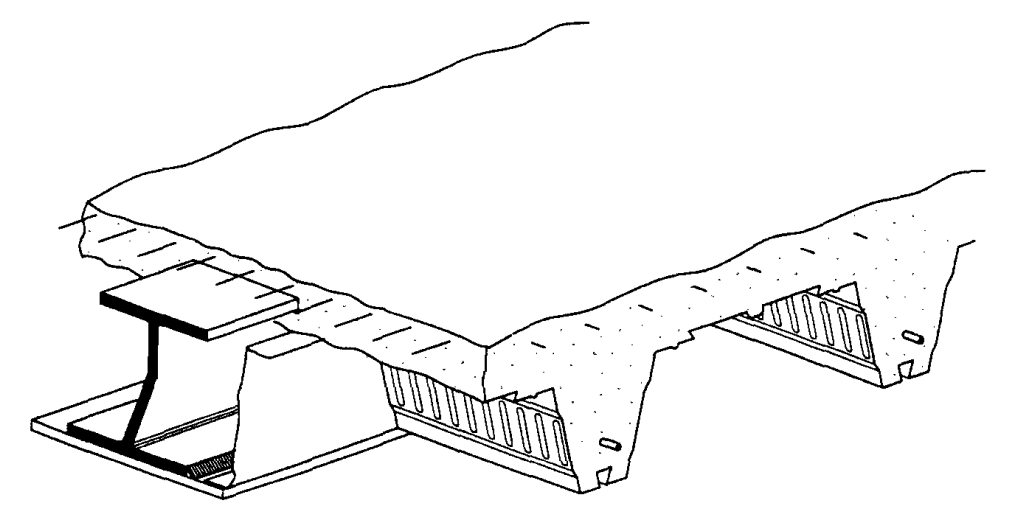
\includegraphics[width=\textwidth, height=5cm]{figures/slimflor.png} 
\caption{SlimFlor beam}
\label{fig:slimflor}
\end{subfigure}
\begin{subfigure}{0.49\textwidth}
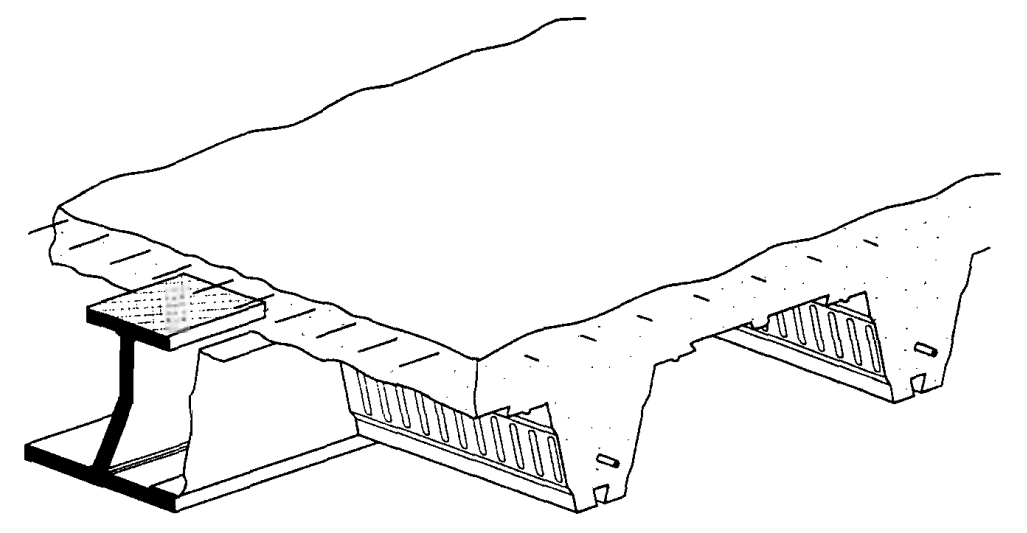
\includegraphics[width=\textwidth, height=5cm]{figures/slimdek.png}
\caption{SlimDek floor system}
\label{fig:slimdek}
\end{subfigure}
\caption{SlimFlor vs SlimDek (ASB) systems \citep{RefWorks:lawson1999slimflor}}
\label{fig:slimfloorvsasb}
\end{figure}

Aside from the basic slim floor system, many manufacturers have created their own systems that either change the beam section or shear connection to achieve different structural performances. \cite{RefWorks:arcelormittal2017slimfloor} introduced the Composite Slim Floor Beam (CoSFB) as a new development into improving shear transfer between the steel beam and the surrounding concrete. This system uses web opening in the steel beam to allow concrete to pass through the web, forming concrete dowels that provide shear connection between the beam and the slab. It also increases the allowable span from approximately 10 to 12 m while also reducing the slab depths compared to standard slim-floor beams \citep{RefWorks:ahmed2019evolution}. The CoSFB system can also be used with the Cofradal slab system as well as standard steel decking.
 
\cite{RefWorks:2024deltabeam} developed the DELTABEAM system which consists of a hollow steel box section with regularly spaced web openings. Similar to CoSFB, concrete passes through these openings to enable composite action. This system can achieve a span of 13.5 m with a structural depth of 500 mm and can achieve a fire resistance of 60 minutes and vibration performance of 3 Hz but more studies are required due to the configuration complexity \citep{RefWorks:peltonen2012connection}.

\cite{RefWorks:ju2003structural} researched a new type of slim floor beam known as i-TECH beams. It consisted of an asymmetric steel beam with web openings, formed through welding a top plate to a bottom tee-section. Non-structural channels are also fixed to the bottom flange of the steel beam to support the deck. Instead of using shear connectors, composite action is achieved through the bond strength of the interface between the concrete slab and the steel beam. The beam can span from 7.5 to 15m with a depth of 300mm however it only reaches a fire resistance of 40 minutes which is less than that provided by SlimFlor  beams \citep{RefWorks:ju2009flexural}.

Another example is the Ultra Shallow Floor Beam (USFB) developed by Westok. This system consists of two asymmetric tee-sections welded together to form a cellular beam with web openings. Similar to other recent systems, composite action is achieved through concrete dowel connections. It is also recommended to provide rebars within the openings to improve the continuity of the slabs on either side of the beam \citep{city1965}. USFB systems can achieve spans of up to 10 m with a depth of 300 mm, outperforming the other shallow floor beams presented \citep{RefWorks:ahmed2019evolution}.

\begin{figure}[h]
 \begin{subfigure}{0.49\textwidth}
     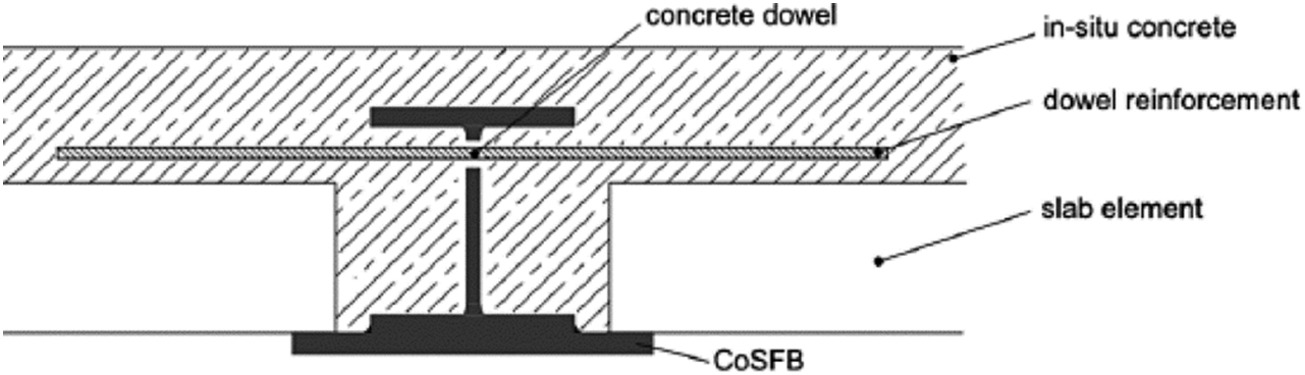
\includegraphics[width=\textwidth]{figures/Cosfb.jpg}
     \caption{CoSFB}
     \label{fig:cosfb}
 \end{subfigure}
 \hfill
 \begin{subfigure}{0.49\textwidth}
     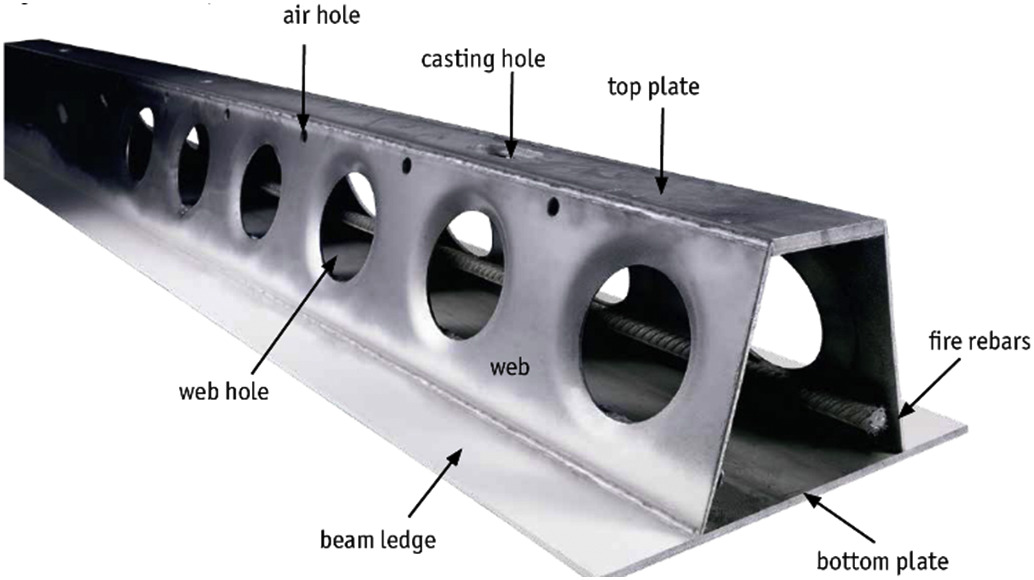
\includegraphics[width=\textwidth]{figures/deltabeam.jpg}
     \caption{DELTABEAM}
     \label{fig:delta}
 \end{subfigure}
 
 \medskip
 \begin{subfigure}{0.49\textwidth}
     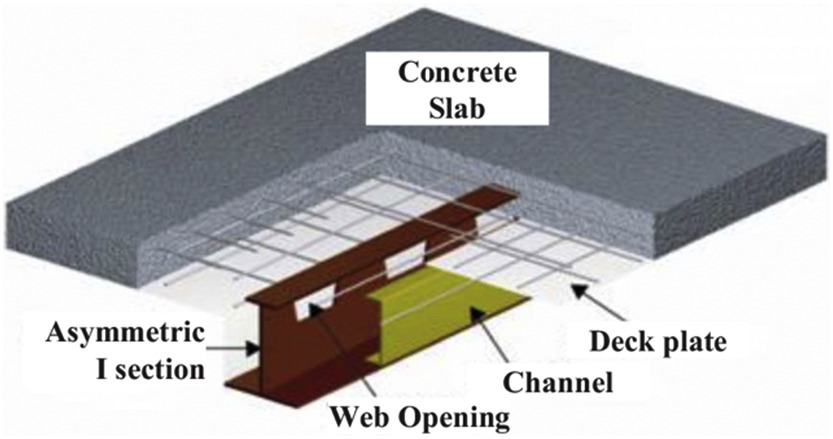
\includegraphics[width=\textwidth]{figures/itech.jpg}
     \caption{ITECH}
     \label{fig:itech}
 \end{subfigure}
 \hfill
 \begin{subfigure}{0.49\textwidth}
     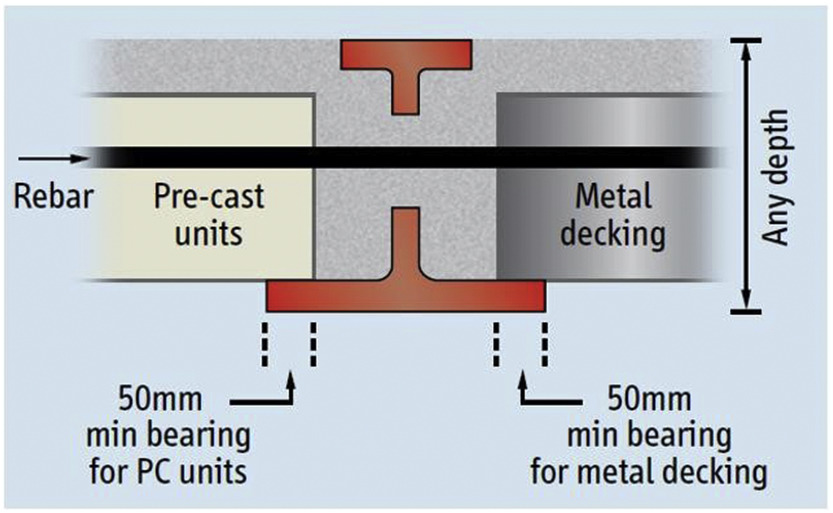
\includegraphics[width=\textwidth]{figures/USFB.jpg}
     \caption{USFB}
     \label{fig:usfb}
 \end{subfigure}

 \caption{Recent developments in Slim-floor systems, adopted from \citep{RefWorks:ahmed2019evolution}}
 \label{fig:advanced slimfloor}
\end{figure}

\begin{table}[h]
\centering
\scriptsize
\caption{Flooring system types, adopted from \citep{RefWorks:ahmed2019evolution}}
\label{tab:slimfloor_comparison}
\begin{tabularx}{\textwidth}{p{2cm}XXXXXXX}
\toprule
 & Composite downstand beam & SlimFlor beam & ASB & ITECH & DELTABEAM & USFB & CoSFB \\
\midrule

Type of shear connection &
Shear stud connection &
Shear stud connection &
Using top flange embossment connections &
Bearing concrete passing through the web opening shear connection &
Bearing concrete passing through the web opening shear connection &
Plug composite action shear connection &
Concrete dowel shear connection \\

Span limitation (m) &
4-6 with metal deck; 6-12 with HCU &
5-10 &
6-7.5 &
7.5-15 &
Up to 13.5 &
Up to 10 &
Up to 12 \\

Depth limitation (mm) &
steel depth + (120-160) mm slab depth &
280-320 &
310-340 &
300 and $>$300 &
200-500 &
300 &
350 \\

Fire performance (min) &
30-240 &
60 &
90 &
40 &
60 &
40 &
60 \\

Vibration performance (Hz) &
N.A.$^\dagger$ &
N.A.$^\dagger$ &
N.A.$^\dagger$ &
$>3$ &
$>3$ &
$>3$ &
$>3$ \\

\bottomrule
    \end{tabularx}
    \vspace{4pt}
    {\footnotesize
    $^\dagger$ Vibration performance figures are not published in
    standard tabular form for conventional downstand composite
    beams, SlimFlor beams, or ASB systems; assessment is carried
    out using a calculation-based approach per \citet{RefWorks:hicks2009p354}.
    The published $>3$~Hz values for ITECH, DELTABEAM, USFB,
    and CoSFB are minimum natural frequency targets drawn from
    manufacturer technical documentation.
    }
\end{table}

These developments demonstrate the ongoing research into slim floor construction, with the aim being to optimise structural performance while reducing construction depth and improve constructibility. The systems discussed are summarised in Table~\ref{tab:slimfloor_comparison} and Figure~\ref{fig:advanced slimfloor}. Although there is a large number of slim floor systems that have been developed, not all are equally suitable for inclusion in the optimisation tool. In particular, complex systems such as DELTABEAM and iTECH rely on non-standard beam geometries which can limit the availability of publicly accessible design tables and product properties needed for implementation. In contrast, systems such as the standard slim floor and 'SlimDek' are based largely on standard hot rolled steel sections which makes the structural behaviour and design procedures easier to implement. 

Another important consideration is the availability of environmental data required for the sustainability objective. Three manufacturers are currently represented in the database: Tata Steel (ComFlor range), ArcelorMittal (Cofraplus range), and Kingspan (Multideck range). All three provide published EPDs and comprehensive design data through technical manuals or proprietary software \citep{RefWorks:2017comflor, RefWorks:2021floors, RefWorks:kingspan2026multideck}. These datasets allow the GWP contribution of each deck product to be quantified from verified manufacturer data. It should be noted, however, that the granularity of available EPD data varies between manufacturers: Tata Steel provide individual declarations for each \mbox{ComFlor} profile, whereas ArcelorMittal and Kingspan each publish a single EPD covering their entire decking range. The implications of this for the environmental assessment are discussed further in Chapter~\ref{thirdchapter}.

Furthermore, SlimFlor beam and SlimDek floor systems have been used in European steel-framed construction and are supported by comprehensive design guidance and technical manuals published by the manufacturers. The availability of established design methods makes these systems particularly suitable for parametric analysis and optimisation. For these reasons, this research focuses primarily on composite downstand, SlimFlor and SlimDek floor systems. The following section therefore reviews the structural design procedures used for composite slabs and slim floor systems, which form the basis of the optimisation methodology developed in this study.
%---------------------------------------------------------------
\subsection{Design Methods}
%---------------------------------------------------------------
The design of composite steel-concrete slabs is governed by the interaction between steel and concrete under both construction and composite loading conditions. In European practice, the design of composite steel and concrete structures is carried out in accordance with Eurocode 4 \citep{RefWorks:cen2004en4}, used alongside Eurocode 2 \citep{RefWorks:cen2004en2} for concrete elements and Eurocode 3 \citep{RefWorks:cen2005en3} for structural steel components. The Eurocodes are a series of standards providing design rules for all common structure types; they are referenced in this report as, for example, 4-1-1/9.4, meaning Clause 9.4 of EN 1994-1-1.

Composite floor systems must be verified for both ultimate limit states (ULS) and serviceability limit states (SLS, comprising crack control, deflection, and vibration), as well as for fire resistance and acoustic performance. A defining feature of their design is its staged nature, which requires the verification of two distinct conditions: the construction stage, in which the wet concrete is supported by the bare steel deck acting as formwork, and the final composite stage, in which the hardened concrete and the deck act together. A further complication is that, in practice, design resistances are frequently derived from manufacturer test data rather than by calculation alone, since the local buckling behaviour of thin profiled sheeting is difficult to capture analytically.

\subsubsection*{Construction stage}
During the construction stage the concrete has not yet hardened and therefore does not contribute to the resistance of the slab; this is often the limiting stage of the design. The steel deck must carry the wet concrete, construction loads, and its own self-weight while acting as falsework. Where deck deflections become significant, an additional load due to ponding of the wet concrete must be considered. Two construction methods are possible. In \textit{unpropped} construction the deck spans unsupported between beams, and for continuous decks the support moments may be partially redistributed into the span. In \textit{propped} construction temporary props carry the wet concrete, permitting thinner slabs and lighter deck profiles, but at the expense of slower construction; in this case no moment redistribution at ULS is permitted \citep{RefWorks:hicks2008en}. The bending, shear, and deflection resistances of the bare deck are specified in Eurocode 3, although manufacturers commonly publish test-derived resistances determined in accordance with EN~1993-1-3 Annex~A, which are less conservative than the analytical effective-width approach.

\subsubsection*{Composite stage}
Once the concrete has hardened, the slab and deck act compositely through longitudinal shear transfer at the steel--concrete interface. The composite section benefits from greatly increased stiffness and bending resistance. The degree of shear connection governs whether full or partial composite action develops; full connection is generally only achievable at longer spans, with the shear bond often being the critical mechanism at shorter spans, in which case only partial composite action is mobilised. Eurocode 4 provides plastic stress-block methods for the sagging moment resistance under both full and partial shear connection.

The longitudinal shear resistance at the steel--concrete interface is assessed using empirical methods, since it cannot be reliably predicted analytically. Two approaches are recognised: the m--k method and the partial connection method. Both rely on standardised slab tests in which the specimens are first cycled to remove the chemical bond, leaving only the mechanical and frictional interlock, and then loaded to failure \citep{RefWorks:stark1990plastic}. The partial connection method yields a characteristic shear bond strength $\tau_{u,Rk}$, whereas the m--k method establishes two empirical constants, $m$ and $k$, representing the mechanical and frictional interlock respectively, from a linear regression of two groups of tests \citep{RefWorks:porter1976design}. \citet{RefWorks:bode1993modern} note several deficiencies of the m--k approach: it is not based on a mechanical model and is therefore less flexible than the partial connection method, its constants conflate all influencing parameters such that they cannot be separated, and it cannot quantify the benefit of additional reinforcement. The shear connection may be enhanced by end anchorage, either by welded headed studs or by deformation of the deck ends, although Eurocode 4 provides design rules only for through-deck welded studs (4-1-1/9.7.4); in practice such connectors are seldom credited in manufacturer design tables, giving a conservative result.

Vertical shear and, where concentrated loads are present, punching shear are verified using the Eurocode 2 provisions for the concrete section, treating the deck and any additional support reinforcement as tensile reinforcement. Serviceability is frequently the controlling consideration for floor slabs: deflection and vibration limits, specified by Eurocode 4 and the relevant National Annex, often govern the final design, particularly at longer spans. The specific limits, partial factors, and the detailed procedures adopted in the present model are set out in Chapter~\ref{thirdchapter}.

\subsubsection*{Vibration}
The principal UK guidance for assessing the vibration serviceability of composite floors is SCI~P354 \citep{RefWorks:hicks2009p354}, which adopts a response-factor approach based on the dynamic response of the floor to walking excitation. The method first determines the fundamental natural frequency $f_0$ of the floor system, accounting for the combined stiffness and mass of the slab and its supporting beams. Floors are then classified by this frequency: \emph{low-frequency} floors (typically $f_0 \lesssim 10$\,Hz) are susceptible to resonance, in which successive footfalls coincide with a harmonic of the walking rate and the response builds up over time, whereas \emph{high-frequency} floors respond transiently to each individual footfall as a series of decaying impulses. A minimum frequency of around 3\,Hz is generally required to avoid the most onerous resonant behaviour.

For each case, the method estimates the modal mass participating in the governing mode, derived from the effective floor area mobilised by the walking path, the floor mass per unit area, and the damping ratio $\zeta$ (taken from tabulated values according to occupancy and fit-out, SCI~P354 Table~4.1), and from this computes the root-mean-square acceleration response to a representative walking force. The acceleration is expressed as a dimensionless response factor $R$, defined relative to the baseline human perception threshold for vertical vibration in BS~6472, and is compared against limiting values that depend on the use of the space (for example, $R \le 8$ for general offices, with stricter limits for sensitive environments). Because the method requires bay-level inputs --- secondary and primary beam spans, bay width, number of adjacent bays, and damping --- that fall outside the scope of a slab-only optimisation, only an indicative slab-alone natural frequency check is incorporated in this study, as discussed in Chapter~\ref{thirdchapter}.

\subsubsection*{Acoustic performance}
Acoustic performance is a further design requirement for floor systems. The two phenomena of concern are airborne sound transmission and impact sound transmission. Single-number ratings are derived from frequency-band measurements in accordance with \citet{RefWorks:isoEN7171} (airborne) and \citet{RefWorks:isoEN7172} (impact), and may be predicted from element performance data using \citet{RefWorks:en12354}. Airborne insulation can be expressed either as the weighted (apparent) sound reduction index $R_\mathrm{w}$ ($R'_\mathrm{w}$ in situ), which characterises the element itself, or as the weighted standardised level difference $D_\mathrm{nT,w}$, which is a field quantity that also accounts for the geometry of the receiving room. Impact sound is rated by the weighted standardised impact sound pressure level $L'_\mathrm{nT,w}$. Spectrum adaptation terms ($C$, $C_\mathrm{tr}$, $C_\mathrm{i}$) may be added to emphasise particular source spectra, $C_\mathrm{tr}$ in particular penalising poor low-frequency performance.

Performance requirements and the descriptors used to express them vary between national standards and intended use. In the United Kingdom, Approved Document~E to the Building Regulations \citep{RefWorks:adePartE} specifies field-measured requirements for separating floors between new-build dwellings of $D_\mathrm{nT,w} + C_\mathrm{tr} \geq 45$~dB for airborne insulation and $L'_\mathrm{nT,w} \leq 62$~dB for impact insulation. In Switzerland, SIA~181 \citep{RefWorks:sia181} expresses its requirements using a standardised level difference descriptor and sets them according to a classification of the sensitivity of the receiving space and the noise exposure. For non-residential spaces such as offices, both jurisdictions relax the airborne requirement.

The structural slab provides the primary contribution to airborne sound insulation through its mass per unit area, in accordance with the mass law. Composite slabs using profiled steel decking tend to have lower mass per unit area than solid reinforced concrete slabs of equivalent structural depth, owing to the void volume within the deck ribs. As a result, composite floor systems often require supplementary acoustic treatment --- typically a floating screed over a resilient layer --- to satisfy impact sound requirements and, in higher-specification applications, to meet airborne insulation targets as well \citep{RefWorks:scip300}. Since the acoustic performance of the floor depends heavily on the non-structural build-up layers rather than the structural cross-section alone, the choice of floor build-up in this study is informed by the acoustic requirements of each occupancy scenario, as discussed further in Chapter~\ref{thirdchapter}.

\subsubsection*{Fire resistance}
Fire resistance is a critical design requirement for structural floor systems. Composite slabs and slim floor systems generally perform well in fire owing to the presence of the concrete, but design is still carried out in accordance with Eurocode 4. Slim floor systems offer a particular advantage because the steel beam is partially or fully encased within the concrete slab, which reduces the rate of temperature rise in the steel and can eliminate the need for applied fire protection; ratings of 60 to 90 minutes are commonly achievable without protection, depending on slab thickness and reinforcement \citep{RefWorks:hicks2008en}. EN~1994-1-2 (4-1-2/4.3.1) \citep{RefWorks:cen2005en} governs the fire design of composite slabs, with detailed checks for moment resistance and thermal insulation given in its Annex~D; the UK provides alternative guidance under \citet{RefWorks:francis2013ncci}, on which some manufacturers base their design. Thermal insulation is satisfied by providing a minimum slab thickness that depends on the deck profile (re-entrant or trapezoidal) and the concrete type. Most manufacturers publish fire design tables based on the detailed calculation methods of their home-country standards --- either the Eurocodes or the now-withdrawn British Standards.

\subsubsection*{Manufacturer design resources}
In practice, the design of composite slabs and slim floor systems is strongly supported by manufacturer technical manuals, design tables, and dedicated software, which translate the code rules into practical engineering solutions and are widely used for preliminary design and verification. \citet{RefWorks:2017comflor}, \citet{RefWorks:2021floors}, and \citet{RefWorks:kingspan2026multideck} are examples of manuals providing pre-calculated tables of allowable spans, load capacities, slab depths, reinforcement requirements, and fire ratings for standard configurations, enabling rapid system selection without detailed hand calculation. However, these tables are based on discrete parameter sets, restricting the exploration of non-standard configurations, and proprietary software often limits transparency in the underlying calculations. Both characteristics constrain their use in a custom optimisation framework, where explicit control over input parameters and calculation methods is required --- motivating the transparent, parametric implementation of the design checks developed in this study and described in Chapter~\ref{thirdchapter}.

%---------------------------------------------------------------
\subsection{Synthesis and Research Gaps}
%---------------------------------------------------------------
The literature reviewed in this chapter highlights the increasing importance of reducing embodied carbon within structural design. Structural systems, and in particular floor slabs, represent a significant proportion of the total material consumption in multi-storey buildings and therefore offer substantial potential for reducing environmental impact through improved material efficiency and system selection.

Composite construction has emerged as an effective strategy for improving structural efficiency by combining the advantageous properties of steel and concrete. The development of composite floor systems, including profiled steel decking and shear connection technologies, has enabled widespread adoption in modern construction. More recently, slim floor systems have been developed to further improve structural efficiency by integrating steel beams within the slab depth, reducing overall floor height while maintaining structural performance.

A range of slim floor systems have been identified in the literature, including SlimFlor, SlimDek, CoSFB, and Delta beam systems. These systems offer varying performance in terms of span capabilities, structural depth, and construction efficiency. However, their design is typically supported by manufacturer-specific guidance, technical manuals, and software tools, which are largely based on the design principles outlined in Eurocode standards. While these tools facilitate practical design, they are generally oriented towards discrete design solutions and may limit flexibility when exploring a wider design space.

Although previous research has investigated the optimisation of structural systems with respect to material use and environmental impact, the majority of studies have focused on conventional reinforced concrete slabs. Comparatively limited research has been identified that examines the environmental performance of steel–concrete composite slab systems, and in particular slim floor configurations, within an optimisation framework. Furthermore, existing design tools are not typically structured to directly incorporate environmental performance metrics such as Global Warming Potential into the design process.

Another limitation identified in the literature is the reliance on discrete design tables and proprietary software tools, which restrict the ability to explore continuous design variables and understand the influence of individual parameters. While these tools are effective for practical design, they lack the transparency and flexibility required for parametric optimisation studies. This highlights the need for a more adaptable modelling approach that integrates structural design checks with environmental assessment in a unified framework.

Based on these observations, a clear research gap exists in the development of a parametric and optimisation-based approach for evaluating composite slim floor slab systems with respect to embodied carbon. This research therefore aims to address these gaps by developing a parametric structural model for slim floor slab systems, enabling systematic evaluation and optimisation of their environmental performance. The focus on widely used systems such as SlimFlor and SlimDek ensures that the results remain relevant to current engineering practice while allowing sufficient flexibility for detailed analysis.
    \section{Methodology}
\label{thirdchapter}

%===============================================================
\subsection{Introduction}
%===============================================================
This chapter presents the methodology developed to evaluate and optimise composite steel--concrete floor slabs with respect to Global Warming Potential (GWP). The approach extends an existing parametric optimisation framework, originally developed by the Chair of Concrete Structures and Bridge Design at ETH Zurich for reinforced concrete and timber slab systems, to incorporate composite slab cross-sections. This extension enables the first systematic Eurocode-compliant comparison between conventional reinforced concrete flat slabs and composite slabs across a range of practical span lengths and occupancy scenarios. The methodology is implemented in Python and structured around a relational database of commercially available deck and concrete products, from which minimum-GWP cross-sections are identified for each span using a scalar bounded optimisation algorithm. The overall workflow, including the loop structure, the optimisation step, and the limit-state checks, is summarised in Figure~\ref{fig:code_flowchart}.

The chapter is structured as follows. Section~\ref{sec:prior_work} describes the pre-existing framework that this work extends. Section~\ref{sec:database} details the material and product database. Section~\ref{sec:casestudies} defines the case studies, including loading scenarios and floor build-ups. Section~\ref{sec:design_vars} sets out the design variables and design parameters. Section~\ref{sec:design_procedure} presents the structural verification procedure with the governing equations for each limit state, followed by the fire and acoustic design provisions. Section~\ref{sec:env_impact} outlines the environmental impact calculation. Section~\ref{sec:optimisation} describes the optimisation algorithm and convergence behaviour. Section~\ref{sec:validation} reports the validation against manufacturer design tables. Finally, Section~\ref{sec:assumptions} sets out the principal assumptions and limitations of the methodology.

%===============================================================
\subsection{Pre-existing framework}
\label{sec:prior_work}
%===============================================================
The composite slab module developed in this study is integrated into a pre-existing Python optimisation framework developed at the Chair of Concrete Structures and Bridge Design. The pre-existing framework provides cross-section classes for reinforced concrete rectangular slabs, reinforced concrete rib slabs, and several timber typologies (rectangular, box, and ribbed sections). For each typology, the framework performs ultimate limit state, serviceability limit state, and fire design checks in accordance with the relevant Eurocodes and Swiss standards, and quantifies GWP, cost (work in progress), and material quantities for use as objective functions in the optimisation.

The code is organised into two layers. The \textit{cross-section layer} (\texttt{struct\_analysis.py}) holds material and geometric properties for a given cross-section and evaluates section-level resistances and limit state checks. Each cross-section type (e.g.\ \texttt{RCSlab}, \texttt{TimberSlab}, \texttt{CompositeSlab}) is implemented as a class; instantiating it with a set of design parameters computes all relevant properties and runs the applicable checks. The \textit{member layer} (\texttt{struct\_optimization.py} and the per-configuration scripts) drives the optimisation: it iterates over spans, deck products, and concrete grades, instantiates cross-sections, and calls the optimiser to minimise the objective function (GWP) subject to structural feasibility. This separation means that structural logic is fully self-contained within each cross-section class and can be tested independently of the optimisation.

The pre-existing database is a SQLite file generated from an Excel workbook, organised into three tables: \texttt{material\_prop} (mechanical properties of concrete, reinforcing steel, and timber grades), \texttt{products} (Environmental Product Declaration data linked to material entries), and \texttt{floor\_struc\_prop} (non-structural floor build-up layer properties). The contribution of the present study to the database structure consists of an additional table, \texttt{sheeting\_prop}, containing the properties of profiled steel decking products required for composite slab design (described in Section~\ref{sec:database}), together with extensions to the \texttt{material\_prop} and \texttt{floor\_struc\_prop} tables to incorporate additional EPD entries and floor build-up layers relevant to composite construction.

The implementation in this study introduces a new \texttt{CompositeSlab} class within the cross-section module \texttt{struct\_analysis.py}, a corresponding optimisation routine \texttt{opt\_comp\_slab} within \texttt{struct\_optimization.py}, and member-level analysis scripts for simply-supported (\texttt{simple\allowbreak\_span\_composite.py}), two-span (\texttt{two\_span\_composite.py}), and three-span (\texttt{three\_span\_composite.py}) configurations, alongside auxiliary scripts for validation, end-anchorage comparison, GWP breakdown plotting, and vibration checking.

%===============================================================
\subsection{Material database}
\label{sec:database}
%===============================================================
The optimisation draws on the SQLite database described above. Of the four tables, the \texttt{sheeting\_prop} table is introduced as part of this study; the other three are inherited from the pre-existing framework with additional entries added to support composite slab design. The structure and contents of each table are described below.

\subsubsection*{Decking products (\texttt{sheeting\_prop})}
The decking table contains product-specific mechanical properties required for structural verification: rib geometry parameters $h_p$ (rib height), $l_1$ (rib pitch), $l_2$ (lower flange width), $l_3$ (upper flange width), sheet thickness $t$, web inclination $\theta$, and per-metre cross-sectional area $A_p$ and effective area $A_{p,e}$; section properties $e$ (centroidal axis from soffit), $e_p$ (effective centroidal axis), $I_p$ (second moment of area), $W_{pl}$ (plastic modulus), $W_{el,f}$ (effective elastic modulus); resistance values $M_{c,Rd}$ (sagging moment resistance), $M_{t,Rd}$ (hogging moment resistance, where available), and $f_{ypd}$ (design yield strength). Longitudinal shear parameters are stored where available, in one of two formats depending on the characterisation method adopted by the manufacturer: the m--k constants $(m_p, k_p)$ or the characteristic shear bond strength $\tau_{u,Rk}$ from EN~1994-1-1 Cl.\,9.7.3.

The volume of concrete that fills the trough voids is stored as the parameter $V_\mathrm{tr}$ (in m$^3$/m$^2$), derived from the manufacturer-declared concrete volume per square metre and used in the GWP and self-weight calculations as described in Section~\ref{sec:env_impact}.

Environmental data are stored as a GWP value accompanied by a unit descriptor (\texttt{GWP\_UNIT}), since manufacturer EPDs express results in differing functional units---per unit area (kg\,CO$_2$-eq/m$^2$) or per unit mass (kg\,CO$_2$-eq/t)---and normalisation to a consistent per-metre-length basis is applied within the model.

Deck products currently included in the database are drawn from the ComFlor range produced by Tata Steel, the Cofraplus and Cofradal ranges from ArcelorMittal, and the Multideck range from Kingspan. These manufacturers were selected on the basis of EPD and property availability, coverage of both shallow ($h_p \le 80$\,mm) and deep ($h_p \ge 200$\,mm) decking profiles, and suitability for the span range under investigation, as discussed in Section~\ref{sec:commercial_slim_floor}.

Mechanical property data was obtained from the manufacturer technical manuals \citep{RefWorks:2017comflor, RefWorks:2021floors, RefWorks:kingspan2026multideck} as well as the manufacturers' design software (ComFlor analysis software, COFRA 5 and Kingspan Catalyst respectively), and EPD values were sourced from the corresponding manufacturer-published declarations. 

\subsubsection*{Material properties (\texttt{material\_prop})}
The material property table contains design properties for concrete, timber, and steel: characteristic compressive strength $f_{ck}$, mean tensile strength $f_{ctm}$, mean elastic modulus $E_{cm}$, dry and wet unit weights, and (for reinforcement) characteristic yield strength $f_{sk}$, modulus $E_s$, cross-sectional area per metre $A_s$, and bar diameter $d_s$. For mesh reinforcement, standard fabric types A142, A193, A252, and A393 are listed (per BS~4483:2025). For timber, additional properties such as bending and shear strengths and burn rate are included.

\subsubsection*{Products (\texttt{products})}
The products table is the environmental data library of the framework, inherited from the prior work and extended for this study. Each row holds an Environmental Product Declaration (EPD) entry, or an equivalent life-cycle dataset, for a structural or non-structural material, linked to a mechanical-property entry through the \texttt{MECH\_PROP} key. The table spans the material families used across the framework's slab typologies---ready-mixed concrete, reinforcing steel, structural steel sections, prestressing steel, and engineered timber (glue-laminated, cross-laminated, and solid timber).

For each entry the table records the Global Warming Potential together with metadata establishing its provenance and validity: the data \emph{source}, the EPD identifier with its issue and expiry dates, the country of declaration, the declared density and (for concrete) the cement type and exposure class, and cross-reference identifiers to the KBOB and Ökobaudat catalogues. The GWP is stored not as a single figure but split into life-cycle stages---modules A1--A3 (cradle-to-gate) and C1--C4 (end-of-life)---so that the system boundary adopted in Section~\ref{sec:env_impact} can be assembled consistently from the same underlying data. Flags record whether an entry is a verified EPD and whether it remains within its validity period.

The entries are drawn from many sources, ranging from product-specific to generic:
\begin{itemize}
    \item \textbf{Manufacturer and industry-association EPDs}---verified, product-specific declarations to EN~15804 / ISO~14025. For concrete these include sector EPDs published by the Swiss concrete association (FSKB) for the standard Swiss concrete sorts (NPK~A--G); for reinforcing steel they include producer EPDs from a range of European mills.
    \item \textbf{ecoinvent}---the generic background life-cycle inventory database \citep{RefWorks:ecoinvent2024}, used for Swiss ready-mixed concrete mixes where no product-specific EPD is available. ecoinvent also supplies the background process data underlying the FSKB sector EPDs and the \emph{Betonsortenrechner} concrete-mix calculator entries.
    \item \textbf{KBOB}---the reference dataset \emph{Ökobilanzdaten im Baubereich} \citep{RefWorks:kbob2022} (version~7), published by the Swiss coordination group of public-sector building owners. KBOB provides representative, averaged GWP intensities for common construction materials and is the de-facto reference for embodied-carbon assessment in Swiss practice.
\end{itemize}

The KBOB dataset serves three distinct roles in this study: it provides the GWP intensities for the non-structural floor build-up layers (Section~\ref{sec:floor_buildup}); it provides the representative concrete and reinforcement intensities used for the reinforced-concrete baseline, consistent with the prior framework; and it acts as the independent benchmark against which the manufacturer steel-decking EPDs were assessed, motivating the exclusion of the ArcelorMittal data discussed in Section~\ref{sec:assumptions}.

The GWP of mesh reinforcement is not stored separately in the products table; instead, the GWP per unit mass of B500B reinforcing steel is applied as a representative value, consistent with the treatment of reinforcement in the reinforced-concrete baseline model.

\subsubsection*{Floor build-up (\texttt{floor\_struc\_prop})}
Non-structural floor build-up layers are listed with their height, density, weight, and GWP per unit mass; the per-layer GWP intensities are taken from the KBOB dataset \citep{RefWorks:kbob2022}. The layers used in this study are described in Section~\ref{sec:floor_buildup}. The permanent load contribution of the floor build-up to the composite slab design ($g_{k,\mathrm{fin}}$) is derived directly from the summed self-weight of the declared layers in the database (\texttt{FloorStruc.gk\_area}, in N/m$^2$), ensuring consistency between the GWP calculation and the structural loading used in the optimisation.

%===============================================================
\subsection{Case studies and loading scenarios}
\label{sec:casestudies}
%===============================================================
\subsubsection*{Loading scenarios}

Four occupancy scenarios are evaluated, corresponding to typical multi-storey applications of composite floor systems: \textbf{office}, \textbf{residential}, \textbf{retail}, and \textbf{industrial}. For each scenario, the imposed load $q_k$ and the partition allowance $q_{k,\mathrm{part}}$ are taken from 1-1-1 Table~6.2 according to the use category. The permanent service load $g_{k,\mathrm{serv}}$ represents a fixed services and fittings allowance above the structural slab. Loading parameters for each scenario are summarised in Table~\ref{tab:loading_scenarios}.

\begin{table}[h!]
\small
\centering
\caption{Loading parameters per occupancy scenario.}
\label{tab:loading_scenarios}
\begin{tabular}{lcccccc}
\toprule
Scenario & Cat. & $q_k$ & $q_{k,\mathrm{part}}$ & $g_{k,\mathrm{serv}}$ & $Q_{k,\mathrm{constr}}$ & $\psi_\mathrm{fi}$ \\
         &      & [kN/m$^2$] & [kN/m$^2$] & [kN/m$^2$] & [kN/m$^2$] & [--] \\
\midrule
Residential & A  & 2.0 & ---  & 0.75 & 0.75 & 0.5 \\
Office      & B  & 2.5 & 0.50 & 0.75 & 0.75 & 0.5 \\
Retail      & D1 & 4.0 & ---  & 0.50 & 0.75 & 0.7 \\
Industrial  & E1 & 7.5 & ---  & 0.50 & 0.75 & 0.9 \\
\bottomrule
\end{tabular}
\end{table}

The construction-stage imposed load follows 1-1-6/4.11.2: a uniformly distributed load $Q_{k,1b} = 0.75$\,kN/m$^2$ representing personnel and small equipment is applied across the full span, with an additional $0.75$\,kN/m$^2$ patch load applied over a $3 \times 3$\,m working area (giving a total patch load of $1.5$\,kN/m$^2$) to represent localised concentrations of workers and equipment during pouring. The wet concrete weight $Q_{k,1c}$ is computed from the wet density of the chosen concrete grade and the average concrete depth $h_\mathrm{c,avg}$ (defined in Section~\ref{sec:env_impact}). A minimum base uniform load $Q_{k,1a} = \max(0.75,\;0.10\,Q_{k,1c})$\,kN/m$^2$ is also defined, representing the case where the concrete is heavier than the nominal construction load, to ensure that the construction stage is never under-designed relative to the actual wet concrete weight.

\subsubsection*{Floor build-up}
\label{sec:floor_buildup}

The floor build-up above the structural slab is selected for each occupancy scenario to satisfy the relevant acoustic requirements while minimising additional GWP. The acoustic requirements are taken from SIA~181 \citep{RefWorks:sia181} for the Swiss context and cross-checked against Approved Document E \citep{RefWorks:adePartE} for the UK context, as discussed in Section~\ref{sec:acoustic}. The build-up layers used in this study are listed in Table~\ref{tab:floor_buildup} and shown schematically in Figure~\ref{fig:floor_buildups}.

\begin{figure}[h!]
  \centering
  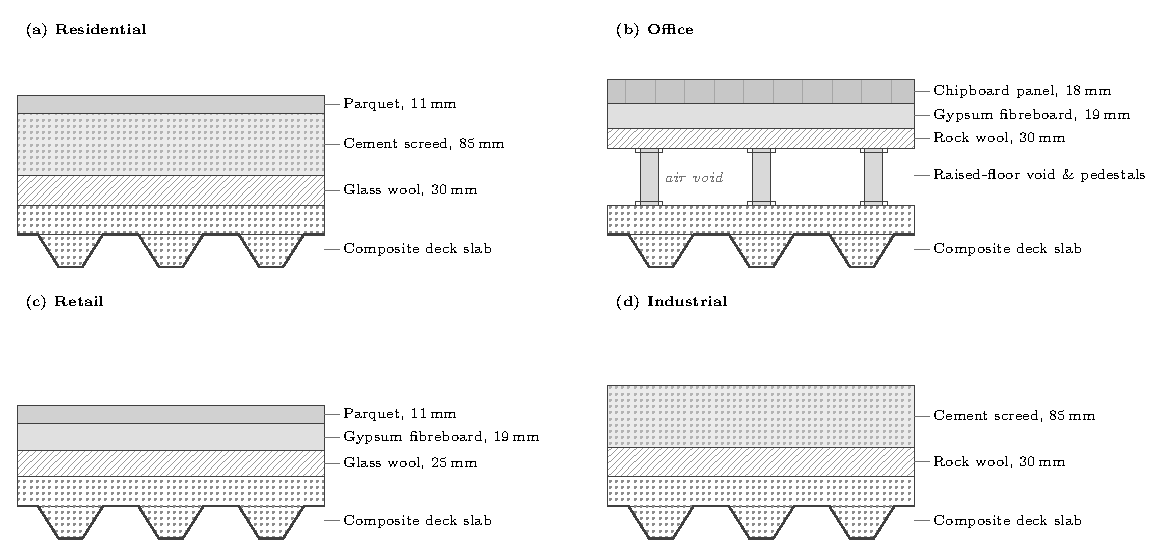
\includegraphics[width=\textwidth]{figures/floor_buildups.pdf}
  \caption{Schematic cross-sections of the floor build-up adopted for each occupancy scenario, shown above the composite steel deck slab. Vertical proportions are exaggerated for clarity and are not to scale. Hatching denotes material type: dotted for cementitious layers (screed and concrete), diagonal for mineral-wool insulation, and solid grey for boards and parquet finishes.}
  \label{fig:floor_buildups}
\end{figure}

\begin{table}[h!]
\small
  \centering
  \caption{Floor build-up layers per occupancy scenario (top to bottom, above structural slab).}
  \label{tab:floor_buildup}
  \begin{tabular}{llccc}
    \toprule
    Scenario & Layer (top to bottom) & Thickness [mm] & Density [kg/m\textsuperscript{3}] & GWP [kg\,CO\textsubscript{2}/kg] \\
    \midrule
    \multirow{3}{*}{Residential}
      & 2-layer factory-sealed parquet & 11 & 555  & 1.28 \\
      & Cement screed                  & 85 & 1850 & 0.12 \\
      & Glass wool insulation          & 30 & 80   & 1.10 \\
    \cmidrule(lr){1-5}
    \multirow{3}{*}{Office}
      & Chipboard panel       & 18 & 640  & 0.53 \\
      & Gypsum fibreboard     & 19 & 1200 & 0.55 \\
      & Rock wool insulation  & 30 & 38   & 0.82 \\
    \cmidrule(lr){1-5}
    \multirow{3}{*}{Retail}
      & 2-layer factory-sealed parquet & 11 & 555  & 1.28 \\
      & Gypsum fibreboard              & 19 & 1200 & 0.55 \\
      & Glass wool insulation          & 25 & 80   & 1.10 \\
    \cmidrule(lr){1-5}
    \multirow{2}{*}{Industrial}
      & Cement screed        & 85 & 1850 & 0.12 \\
      & Rock wool insulation & 30 & 38   & 0.82 \\
    \bottomrule
  \end{tabular}
\end{table}

\subsubsection*{Span ranges and configurations}
The slab is evaluated as a one-way spanning system across spans of 3--10\,m in 1\,m increments, encompassing the practical range for both shallow ($h_p \le 80$\,mm) and deep ($h_p \ge 200$\,mm) decking profiles. Three span configurations are evaluated for each loading scenario:
\begin{itemize}
    \item Single span (simply supported)
    \item Two-span continuous
    \item Three-span continuous
\end{itemize}
Multi-span configurations use equal spans throughout; the influence of unequal spans is not investigated. All structural verification and optimisation is carried out on a per-metre-width basis, allowing results to be expressed as GWP per metre of span length in kg\,CO$_2$-eq/m.

%===============================================================
\subsection{Design variables and parameters}
\label{sec:design_vars}
%===============================================================
The optimisation considers three categories of design variable, summarised in Table~\ref{tab:opt_variables}. The single continuous variable $h$ is optimised by the bounded scalar algorithm; discrete variables are enumerated in an outer loop over all admissible options.

\begin{table}[h!]
\small
\centering
\caption{Optimisation variables and their treatment}
\label{tab:opt_variables}
\begin{tabular}{p{5cm} p{2.5cm} p{2cm} p{4cm}}
\toprule
\textbf{Variable} & \textbf{Symbol} & \textbf{Type} & \textbf{Range / set} \\
\midrule
Total slab depth                  & $h$            & Continuous & $h_p + 50$\,mm $\le h \le 500$\,mm \\
Steel deck product                & ---            & Discrete (enum.) & All products in \texttt{sheeting\_prop} \\
Concrete grade                    & $f_{ck}$       & Discrete (enum.) & C25/30, C30/37 \\
Mesh reinforcement                & $A_s$          & Discrete (auto-selected) & A142, A193, A252, A393 \\
Trough bar diameter (fire only)   & $\varnothing_\mathrm{tr}$ & Discrete (auto-selected) & 8, 10, 12, 16, 20\,mm \\
\bottomrule
\end{tabular}
\end{table}

The minimum permissible total depth is the deck rib height $h_p$ plus a minimum concrete cover of 50\,mm above the top of the ribs, in accordance with 4-1-1/9.2.1, and not less than 90\,mm. The upper search bound is 500\,mm, accommodating the deepest deck profiles at long spans. Both propped and unpropped construction are evaluated: the optimiser first attempts unpropped construction; if no feasible solution exists within the search bounds, a second pass with propped construction is performed.

The mesh reinforcement is selected automatically as the lightest fabric type satisfying the minimum longitudinal reinforcement ratio of 4-1-1/9.8.1, namely $0.2\%\,A_c$ for unpropped construction (or $0.4\%\,A_c$ if propped). The hogging ULS check at internal supports (Section~\ref{sec:hogging}) and the fire D2/D3 checks (Section~\ref{sec:fire}) may upgrade the mesh to a heavier fabric if required.

Trough bar reinforcement within the deck ribs is not considered for structural ULS checks. The fire design procedure (Section~\ref{sec:fire}) selects the minimum trough bar diameter required for the sagging moment check at elevated temperature; if no diameter from the available set produces a passing fire check, the cross-section is recorded as failing the D2 check.

Table~\ref{tab:design_parameters} summarises the design parameters held constant across all configurations. All quantities in the \texttt{material\_prop} and \texttt{floor\_struc\_prop} tables follow the SI convention adopted throughout this tool (N, m). The \texttt{sheeting\_prop} table follows the engineering convention standard in EN 1994-1-1 and manufacturer datasheets: geometric dimensions in mm, second moments of area in cm$^4$/m, cross-sectional areas in mm$^2$/m, strength values in N/mm$^2$, and moment capacities in kNm/m. Internally, the \texttt{CompositeSlab} class converts between these conventions at the point of use.

\begin{table}[h!]
\scriptsize
\centering
\caption{Summary of design parameters, loading assumptions, and partial factors}
\label{tab:design_parameters}
\renewcommand{\arraystretch}{1.3}
\begin{tabular}{p{6.5cm} p{1.8cm} p{2.8cm} p{3.0cm}}
\hline
\textbf{Parameter} & \textbf{Symbol} & \textbf{Value / Assumption} & \textbf{Reference} \\
\hline
\multicolumn{4}{l}{\textit{Construction-stage Loads}} \\
\hline
Construction stage UDL          & $Q_{k,1b}$        & 0.75 kN/m²         & EN 1991-1-6 Cl.\,4.11.2 \\
Construction stage patch load   & $Q_{k,1b,\mathrm{patch}}$ & 1.5 kN/m² over 3$\times$3 m & EN 1991-1-6 Cl.\,4.11.2 \\
\hline
\multicolumn{4}{l}{\textit{Partial Factors}} \\
\hline
Permanent loads                 & $\gamma_G$        & 1.35               & EN 1990 \\
Variable loads                  & $\gamma_Q$        & 1.50               & EN 1990 \\
Concrete                        & $\gamma_C$        & 1.50               & EN 1992-1-1 \\
Reinforcement                   & $\gamma_S$        & 1.15               & EN 1992-1-1 \\
Steel section                   & $\gamma_{M0}$     & 1.00               & EN 1993-1-1 \\
Longitudinal shear              & $\gamma_{VS}$     & 1.25               & EN 1994-1-1 Cl.\,9.7.3 \\
\hline
\multicolumn{4}{l}{\textit{Serviceability Limits}} \\
\hline
Construction stage deflection   & $\delta_\mathrm{constr}$  & $\min(L/180, 20\,\mathrm{mm})$ or $\min(L/130, 30\,\mathrm{mm})$    & EN 1994-1-1 Cl.\,9.3.2; UK NA \\
Composite stage --- total       & $\delta_\mathrm{tot}$     & $L/300$                            & SIA 263$^{\ddagger}$ \\
Composite stage --- variable    & $\delta_\mathrm{var}$     & $\min(L/350, 20\,\mathrm{mm})$    & EN 1994-1-1 Cl.\,9.8.2(4) \\
\hline
\multicolumn{4}{l}{\textit{Cross-section Constraints}} \\
\hline
Minimum concrete cover above deck & ---             & 50\,mm                            & EN 1994-1-1 Cl.\,9.2.1 \\
Minimum total depth              & ---             & $h_p + 50$\,mm; not less than 90\,mm & EN 1994-1-1 Cl.\,9.2.1 \\
Concrete cover to top mesh       & $c_\mathrm{nom}$ & 20\,mm                            & EN 1992-1-1 Cl.\,4.4 \\
\hline
\multicolumn{4}{l}{\textit{Material Properties}} \\
\hline
Effective deck area (where not stated) & $A_{p,e}$ & $0.9\,A_p$ (shallow); $0.5\,A_p$ (deep, $h_p \ge 80$\,mm) & $^{\dagger}$ \\
Creep coefficient                & $\varphi_t$    & EN 1992-1-1 Annex B & EN 1992-1-1 Cl.\,5.4.2.2 \\
Modular ratio (short-term)       & $n_0$          & $E_a / E_{cm}$ & EN 1994-1-1 Cl.\,5.4.2.2 \\
Modular ratio (long-term)        & $n_L$          & $n_0(1 + 1.1\varphi_t)$ & EN 1994-1-1 Cl.\,5.4.2.2 \\
Cement class                     & ---            & N (normal)              & EN 1992-1-1 \\
Relative humidity                & RH             & 50\% (interior)         & EN 1992-1-1 Annex B \\
Loading age                      & $t_0$          & 28 days                 & SCI P359 Cl.\,6.3 \\
\hline
\multicolumn{4}{l}{\textit{Fire Design}} \\
\hline
Fire resistance period           & $R_\mathrm{fi}$    & R60 & EN 1994-1-2 Annex D \\
Fire combination factor          & $\psi_\mathrm{fi}$ & 0.5 -- 0.9 (occupancy-dependent)        & EN 1990 Table A1.1 \\
Trough bar diameter set          & $\varnothing_\mathrm{tr}$ & $\{8, 10, 12, 16, 20\}$\,mm    & --- \\
\hline
\multicolumn{4}{l}{\textit{Environmental Assessment}} \\
\hline
LCA system boundary              & ---            & A1--A3 and C1--C4              & EN 15804 \\
Functional unit                  & ---            & kg\,CO$_2$-eq/m of span length & --- \\
\hline
\end{tabular}
\vspace{4pt}\\
{\footnotesize
$^{\ddagger}$ EN~1994-1-1 Cl.\,9.8.2(4) recommends a total deflection limit of $L/250$; the more conservative limit of $L/300$ is adopted here in accordance with SIA~263 \citep{RefWorks:sia263}, for consistency with the prior framework against which the composite results are compared.\\
$^{\dagger}$ Conservative fallback: $A_{p,e} = 0.9\,A_p$ for shallow profiles ($h_p < 80$\,mm); $A_{p,e} = 0.5\,A_p$ for deep profiles ($h_p \ge 80$\,mm). Where the manufacturer publishes $A_{p,e}$ explicitly it is used directly.
}
\end{table}

%===============================================================
\subsection{Design procedure}
\label{sec:design_procedure}
%===============================================================
Structural verification follows the staged nature of composite construction, distinguishing between the \textbf{construction stage}, in which the concrete is wet and only the steel deck resists loads, and the \textbf{composite stage}, in which the hardened concrete and the deck act together. Checks are performed in accordance with EN~1994-1-1/2 supplemented by EN~1992-1-1 and EN~1993-1-3. The full set of checks evaluated by the model is listed in Table~\ref{tab:checks_summary}.

\begin{table}[h!]
\small
\centering
\caption{Limit state checks performed by the composite slab module}
\label{tab:checks_summary}
\begin{tabular}{p{2.5cm} p{4.0cm} p{6.5cm}}
\toprule
\textbf{Stage} & \textbf{Check} & \textbf{Reference} \\
\midrule
Construction$^{\dagger}$ & ULS bending (sagging) & EN 1993-1-3 Cl.\,5.4.3, EN 1994-1-1 Cl.\,9.3 \\
Construction$^{\dagger}$ & ULS web shear buckling      & EN 1993-1-3 Cl.\,6.1.5 \\
Construction$^{\dagger}$ & SLS deflection              & EN 1994-1-1 Cl.\,9.3.2; UK NA \\
Composite    & ULS sagging moment          & EN 1994-1-1 Cl.\,9.7.2 \\
Composite    & ULS longitudinal shear      & EN 1994-1-1 Cl.\,9.7.3 (m--k) or 9.7.5 ($\tau_u$) \\
Composite    & ULS vertical shear          & EN 1994-1-1 Cl.\,9.7.5; EN 1992-1-1 Cl.\,6.2.2 (2004)\\
Composite    & ULS hogging (cont.\ spans)  & EN 1994-1-1 Cl.\,9.7.3(2)P, 9.4.2(3) \\
Composite    & SLS deflection (total \& variable) & SIA 263; EN 1994-1-1 Cl.\,9.8.2(4) \\
Fire         & D1: thermal insulation      & EN 1994-1-2 Annex D, formula D.1 \\
Fire         & D2: sagging moment $M_\mathrm{Rd,fi}$ & EN 1994-1-2 Annex D, formulae D.4--D.5 \\
Fire         & D3: hogging $M_\mathrm{Rd,fi}$ (cont.) & EN 1994-1-2 Annex D, formulae D.7--D.11 \\
Fire         & D4: minimum effective thickness & EN 1994-1-2 Annex D, Table D.6 \\
Fire         & D5: field of application    & EN 1994-1-2 Annex D, Table D.7 \\
\bottomrule
\end{tabular}
\vspace{2pt}\\
{\footnotesize $^{\dagger}$ For propped construction, a single prop at midspan divides the span into two simply-supported $L/2$ sub-spans during casting (EN~1994-1-1 Cl.\,9.3.1); the construction-stage checks are therefore performed against the $L/2$ sub-span rather than omitted.}
\end{table}

\subsubsection*{Construction stage}
\label{sec:constr_stage}
During unpropped construction the profiled steel deck acts as temporary formwork and must resist the self-weight of the wet concrete, its own self-weight, and the construction imposed loads over the full distance between permanent supports. When propped construction is specified, a single temporary prop is assumed at midspan during casting, dividing each span into two simply-supported $L/2$ sub-spans. The deck still carries the full wet-concrete and construction loads, but over the reduced sub-span $L/2$; the construction-stage checks are therefore not omitted but are evaluated against the $L/2$ sub-span using simply-supported coefficients. Because the propped sub-spans are simply supported, no hogging develops at the permanent internal supports during casting, so the construction-stage hogging and internal-support checks are suppressed for the propped case. The reduced effective span is what makes propped construction feasible at longer spans, where the bare deck could not span the full distance unpropped.

\paragraph{ULS bending.} The construction-stage load model is shown in Figure~\ref{fig:constr_load_model}. The deck is verified against the maximum sagging moment $M_{Ed,sag}$, computed as the more onerous of two construction load cases:
\begin{align}
    M_{Ed,sag,1} &= \alpha_M \cdot w_\mathrm{ULS,1} \cdot L^2
    \label{eq:constr_sag_1} \\
    M_{Ed,sag,2} &= \alpha_M \cdot w_\mathrm{base} \cdot L^2 + M_\mathrm{patch}(q_\mathrm{patch}, a_\mathrm{patch}, L)
    \label{eq:constr_sag_2}
\end{align}
where $w_\mathrm{ULS,1} = \gamma_G G_{k,1a} + \gamma_Q (Q_{k,1a} + Q_{k,1b} + Q_{k,1c})$ combines all construction loads as a full-span UDL, $w_\mathrm{base} = \gamma_G G_{k,1a} + \gamma_Q (Q_{k,1b} + Q_{k,1c})$ is the base UDL excluding the patch enhancement, $q_\mathrm{patch} = \gamma_Q Q_{k,1a}$ is the factored patch load intensity, $a_\mathrm{patch} = 3$\,m, and $M_\mathrm{patch}$ is the mid-span moment contribution from the symmetrically placed patch load. The deck is treated as simply supported at the construction stage, so the sagging coefficient is $\alpha_M = 1/8$ in all cases. For multi-span configurations the deck is assumed to be lapped and effectively pinned over the permanent supports during casting (consistent with the SS treatment in SCI~P300); no continuity moment is taken at this stage. For propped construction the same $\alpha_M = 1/8$ applies, but to the $L/2$ sub-span between the prop and the permanent support (Section~\ref{sec:constr_stage}).

The sagging check is $M_{Ed,sag} \le M_{c,Rd}$, where $M_{c,Rd}$ is the manufacturer-published characteristic sagging moment resistance of the deck. Because the deck is treated as simply supported during casting, no construction-stage hogging check or moment redistribution is performed; the hogging resistance $M_{t,Rd}$ is used only for the composite-stage and fire hogging checks at internal supports (Sections~\ref{sec:hogging} and~\ref{sec:fire}).

\paragraph{ULS shear (web buckling).} Web shear buckling resistance per web is computed in accordance with EN~1993-1-3 Cl.\,6.1.5:
\begin{equation}
    V_{b,Rd,\mathrm{web}} = \frac{h_w \cdot t \cdot f_{bv}}{\sin\theta \cdot \gamma_{M0}}
    \label{eq:web_shear}
\end{equation}
where $h_w = h_p - t$ is the web height, $\theta$ is the web inclination, and $f_{bv}$ is the shear buckling strength obtained from the relative web slenderness $\bar{\lambda}_w = 0.346 \cdot s_w / t \cdot \sqrt{f_{ypd}/E}$:
\begin{equation}
    f_{bv} =
    \begin{cases}
    0.58\,f_{ypd} & \text{if } \bar{\lambda}_w \le 0.83 \\
    0.48\,f_{ypd}/\bar{\lambda}_w & \text{if } 0.83 < \bar{\lambda}_w < 1.40 \\
    0.67\,f_{ypd}/\bar{\lambda}_w^2 & \text{if } \bar{\lambda}_w \ge 1.40
    \end{cases}
    \label{eq:fbv}
\end{equation}
The total resistance is $V_{b,Rd} = N_w \cdot V_{b,Rd,\mathrm{web}}$, where $N_w$ is the number of webs per metre width, taken from the database. The design shear force is the more onerous of the two load-case resultants evaluated at the support.

\paragraph{SLS deflection.} The construction-stage SLS deflection check uses the initial elastic deflection of the bare deck under self-weight $G_{k,1a}$ and wet concrete weight $Q_{k,1c}$ only; construction live loads are excluded per EN~1994-1-1 Cl.\,9.3.2(2):
\begin{equation}
    \delta_\mathrm{initial} = K_\delta \cdot \frac{w_\mathrm{SLS} \cdot L^4}{E \cdot I_p}
    \label{eq:constr_defl}
\end{equation}
with $w_\mathrm{SLS} = G_{k,1a} + Q_{k,1c}$ (characteristic loads) and deflection coefficients $K_\delta = 5/384$ (single span), $2/369$ (two spans), $1/145$ (three or more spans). 

The deflection limit is selected based on whether ponding is significant, following the UK National Annex to EN~1994-1-1:
\begin{equation}
    \delta_\mathrm{limit} =
    \begin{cases}
    \min(L/180,\;20\,\mathrm{mm}) & \text{if } \delta_\mathrm{initial} \le h/10 \quad \text{(Option 1, no ponding)} \\
    \min(L/130,\;30\,\mathrm{mm}) & \text{if } \delta_\mathrm{initial} > h/10 \quad \text{(Option 2, ponding included)}
    \end{cases}
    \label{eq:constr_defl_limit}
\end{equation}
where $h$ is the total slab depth. When Option~2 applies ($\delta_\mathrm{initial} > h/10$), a ponding correction is applied: an extra wet-concrete UDL proportional to the current depression is added, and the resulting increased concrete volume is carried through to the GWP and self-weight calculations.

\begin{figure}[h!]
  \centering
  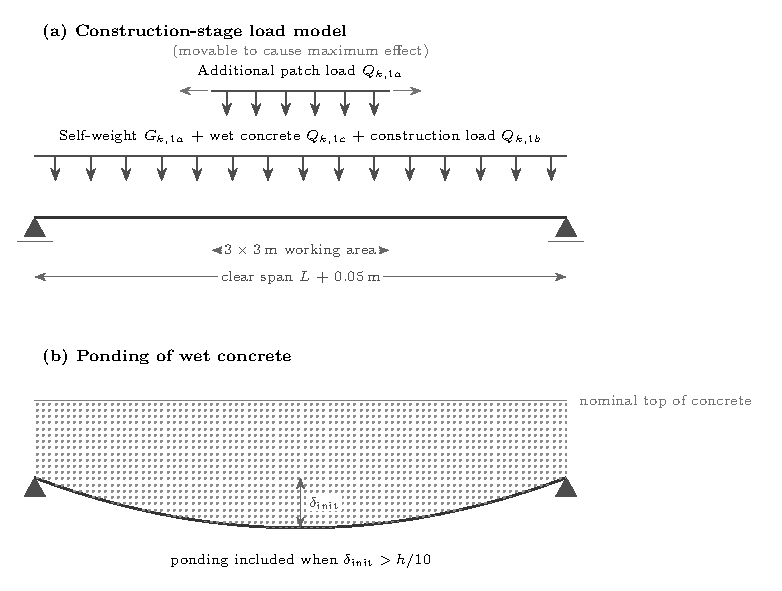
\includegraphics[width=0.9\textwidth]{figures/constr_load_model.pdf}
  \caption[Construction-stage load model]{Construction-stage load model on the profiled steel deck.}
  \label{fig:constr_load_model}
\end{figure}

\subsubsection*{Composite stage}
\label{sec:comp_stage}
Once the concrete has hardened, the slab and the deck act compositely through longitudinal shear transfer at the steel--concrete interface. Composite-stage checks apply to both propped and unpropped construction.

\paragraph{ULS sagging moment.} The composite sagging moment resistance assumes full shear connection and is calculated from a rectangular plastic stress block. The compression force in the concrete is governed by the lesser of the steel deck and concrete capacities:
\begin{equation}
    N_{cf} = \min\!\left(A_{p,e}\,f_{ypd},\; 0.85\,f_{cd}\,b\,h_c\right)
    \label{eq:Ncf}
\end{equation}
The depth of the rectangular concrete compression block is $x_{pl} = N_{cf}/(0.85\,f_{cd}\,b)$, and the plastic sagging moment resistance is:
\begin{equation}
    M_{Rd} = N_{cf} \cdot z / 10^6, \qquad z = h - e_p - \tfrac{1}{2}\,x_{pl}
    \label{eq:comp_mrd_full}
\end{equation}
where $e_p$ is the distance from the soffit to the centroid of the effective deck area. The applied sagging moment is $M_{Ed} = \alpha_{M,\mathrm{sag}}\, w_\mathrm{ULS}\, L^2$, where the elastic moment coefficient $\alpha_{M,\mathrm{sag}}$ depends on the number of spans: $\alpha_{M,\mathrm{sag}} = 1/8$ for a single simply-supported span, $9/128$ for the mid-span of a two-span continuous slab, and $0.080$ for the governing end-span of a three-span continuous slab. The corresponding elastic support (hogging) coefficients are $\alpha_{M,\mathrm{hog}} = 0$, $1/8$, and $0.100$ respectively (Table~\ref{tab:moment_coeffs}). Where hogging redistribution is applied at the internal support (Section~\ref{sec:hogging}), the redistributed surplus is added to the sagging demand, so the moment used in the check is $M_{Ed} = \left(\alpha_{M,\mathrm{sag}} + r\,\alpha_{M,\mathrm{hog}}/2\right) w_\mathrm{ULS}\, L^2$, with $r$ the redistribution factor (zero when no redistribution is applied).

\begin{table}[h!]
\small
\centering
\caption{Elastic moment, shear, and deflection coefficients used for the composite-stage checks, by span configuration (equal spans, uniformly distributed load).}
\label{tab:moment_coeffs}
\begin{tabular}{lcccc}
\toprule
Configuration & $\alpha_{M,\mathrm{sag}}$ & $\alpha_{M,\mathrm{hog}}$ & $\alpha_V$ & $K_\delta$ \\
\midrule
Single span (simply supported) & $1/8$    & $0$     & $1/2$   & $5/384$ \\
Two-span continuous             & $9/128$  & $1/8$   & $5/8$   & $2/369$ \\
Three-span continuous           & $0.080$  & $0.100$ & $0.600$ & $1/145$ \\
\bottomrule
\end{tabular}
\end{table}

\paragraph{ULS longitudinal shear.} Two methods are supported, selected per deck product on the basis of the test data published by the manufacturer.

For decks characterised by m--k constants, the design longitudinal shear resistance per 4-1-1/9.7.3(4) is:
\begin{equation}
    V_{l,Rd} = \frac{b \cdot d_p}{\gamma_{VS}} \left( \frac{m_p \cdot A_p}{b \cdot L_s} + k_p \right)
    \label{eq:mk}
\end{equation}
where $L_s = L/4$ is the shear span for uniformly distributed loading, $b = 1000$\,mm is the unit width, $d_p$ is the effective depth (top of slab to centroid of $A_{p,e}$), and $\gamma_{VS} = 1.25$. The check is $V_{Ed} \le V_{l,Rd}$ where $V_{Ed} = \alpha_V\, w_\mathrm{ULS}\, L$ is the maximum support reaction, with the shear coefficient $\alpha_V$ taken from Table~\ref{tab:moment_coeffs} according to the number of spans.

For decks characterised by the partial connection method (4-1-1/9.7.3(7)), the compression force is:
\begin{equation}
    N_{c} = \tau_{u,Rd} \cdot b \cdot L_x \leq N_{cf}
    \label{eq:partial}
\end{equation}
with $\tau_{u,Rd} = \tau_{u,Rk}/\gamma_{VS}$. For simply-supported spans under UDL, the critical section is at mid-span ($L_x = L/2$). The degree of shear connection is $\eta = N_c/N_{cf}$ where $N_{cf} = A_{p,e} f_{ypd}$ is the full-connection force. The partial-connection moment resistance is:
\begin{equation}
    M_{Rd} = \frac{N_c}{10^6} \cdot z + M_{pr}
    \label{eq:partial_mrd}
\end{equation}
where $z = h - 0.5\,x_{pl} - e_p + (e_p - e)(1 - \eta)$ is the lever arm (mm), $x_{pl} = N_{cf}/(0.85\,f_{cd}\,b)$ is the full-connection compression block depth, and $M_{pr}$ is the reduced plastic moment of the deck section accounting for partial interaction:
\begin{equation}
    M_{pr} = 1.25\,M_{pa}(1 - \eta)
    \label{eq:mpr}
\end{equation}
where $M_{pa}$ is the bending resistance of the profiled steel sheeting (found in the database). The check is $M_{Ed} \le M_{Rd}$ where $M_{Ed} = \left(\alpha_{M,\mathrm{sag}} + r\,\alpha_{M,\mathrm{hog}}/2\right) w_\mathrm{ULS}\, L^2$ using the span-dependent coefficients of Table~\ref{tab:moment_coeffs}.

\paragraph{ULS vertical shear.} Vertical shear is verified per 4-1-1/9.7.5, treating the effective deck area as equivalent tensile reinforcement and using the 2-1-1/6.2.2 (2004) formula for members without shear reinforcement:
\begin{equation}
    V_{Rd,c} = \left[ C_{Rd,c} \cdot k \cdot (100\,\rho_l \cdot f_{ck})^{1/3} + k_1 \cdot \sigma_{cp} \right] \cdot b_w \cdot d
    \label{eq:vrd_c}
\end{equation}
with $C_{Rd,c} = 0.18/\gamma_C$, $k = 1 + \sqrt{200/d_p} \le 2.0$, $\rho_l = A_{p,e}/(b_w \cdot d_p) \le 0.02$, and $\sigma_{cp} = 0$ for unprestressed slabs. A minimum shear resistance is also enforced:
\begin{equation}
    V_{Rd,\min} = v_\mathrm{min} \cdot b_w \cdot d_p, \quad v_\mathrm{min} = 0.035\,k^{1.5}\,f_{ck}^{0.5}
    \label{eq:vrd_min}
\end{equation}
and the design resistance is $V_{Rd,c} = \max(V_{Rd,c},V_{Rd,\min})$.

\paragraph{ULS hogging (continuous spans).}
\label{sec:hogging}
For two- and three-span continuous configurations, an additional hogging check is performed at internal supports. The hogging moment demand is $M_{Ed,hog} = \alpha_H \cdot w_\mathrm{ULS} \cdot L^2$ with $\alpha_H = 1/8$ for two spans and $0.100$ for three spans. The hogging resistance is computed from a plastic stress block with the top mesh reinforcement in tension. Provided the deck is continuous over the support and no plastic redistribution was applied at the construction stage, the profiled deck is permitted to contribute to this compression in accordance with 4-1-1/9.7.2(2)P (see the discussion below); the resistance is then assembled from the mesh tensile force together with the deck and, where required, a concrete compression block:
\begin{equation}
    M_{Rd,hog} = N_\mathrm{deck}\,(d_\mathrm{eff,hog} - e) + N_\mathrm{conc}\,(d_\mathrm{eff,hog} - 0.5\,x)
    \label{eq:hogging}
\end{equation}
where $N_\mathrm{deck} = \min(A_{p,e}\,f_{ypd},\,A_s\,f_{sd})$ is the deck compression force, $N_\mathrm{conc} = \max(A_s\,f_{sd} - N_\mathrm{deck},\,0)$ is any residual concrete compression, $x = N_\mathrm{conc}/(0.85\,f_{cd}\,b)$, $d_\mathrm{eff,hog} = h - c_\mathrm{nom} - n_\mathrm{layers}\,d_s/2$, and $e$ is the gross centroid of the deck from the soffit. Where the deck is ineligible to contribute (deck not continuous, $M_{t,Rd}$ unavailable, or construction redistribution applied), the resistance reduces to the mesh-and-concrete couple $M_{Rd,hog} = A_s\,f_{sd}\,(d_\mathrm{eff,hog} - 0.5\,x)$ with $x = A_s f_{sd}/(0.85\,f_{cd}\,b)$.

If the minimum mesh is insufficient, the mesh is upgraded through the available fabric grades (A142 $\rightarrow$ A193 $\rightarrow$ A252 $\rightarrow$ A393), and if a single layer remains insufficient a double layer is tried, until the check is satisfied; the GWP contribution is updated accordingly.

Where the elastic hogging moment still exceeds the available hogging resistance, elastic moment redistribution is applied in accordance with 4-1-1/9.4.2(3). The support hogging moment is reduced by a redistribution factor $r$, and the corresponding surplus is transferred to the adjacent sagging regions, where it increases the sagging demand by $r\,\alpha_H/2 \cdot w_\mathrm{ULS} L^2$; the sagging checks (Section~\ref{sec:comp_stage}) then use this increased demand. The redistribution factor is capped at $30\%$. If even $30\%$ redistribution is insufficient for the hogging resistance to be satisfied, the hogging check is recorded as failing rather than being forced to unity, so that the configuration is correctly rejected by the optimiser.

\begin{figure}[h!]
    \centering
    % --- (a) Sagging, neutral axis above the steel sheeting ---
    \begin{subfigure}[t]{0.9\textwidth}
        \centering
        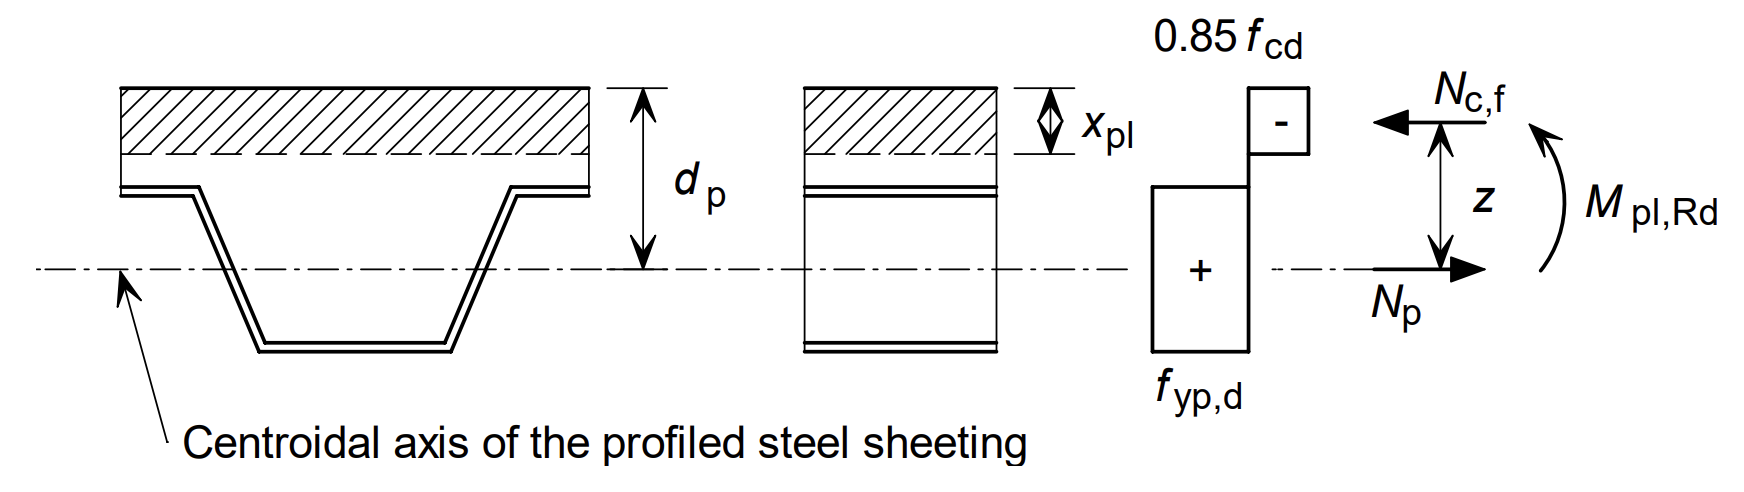
\includegraphics[width=\textwidth]{figures/saggingblockabovesheeting.png}
        \caption{Sagging bending with the plastic neutral axis above the steel sheeting}
        \label{fig:stress_sagging_above}
    \end{subfigure}

    \vspace{1em}

    % --- (b) Sagging, neutral axis within the profile ---
    \begin{subfigure}[t]{0.9\textwidth}
        \centering
        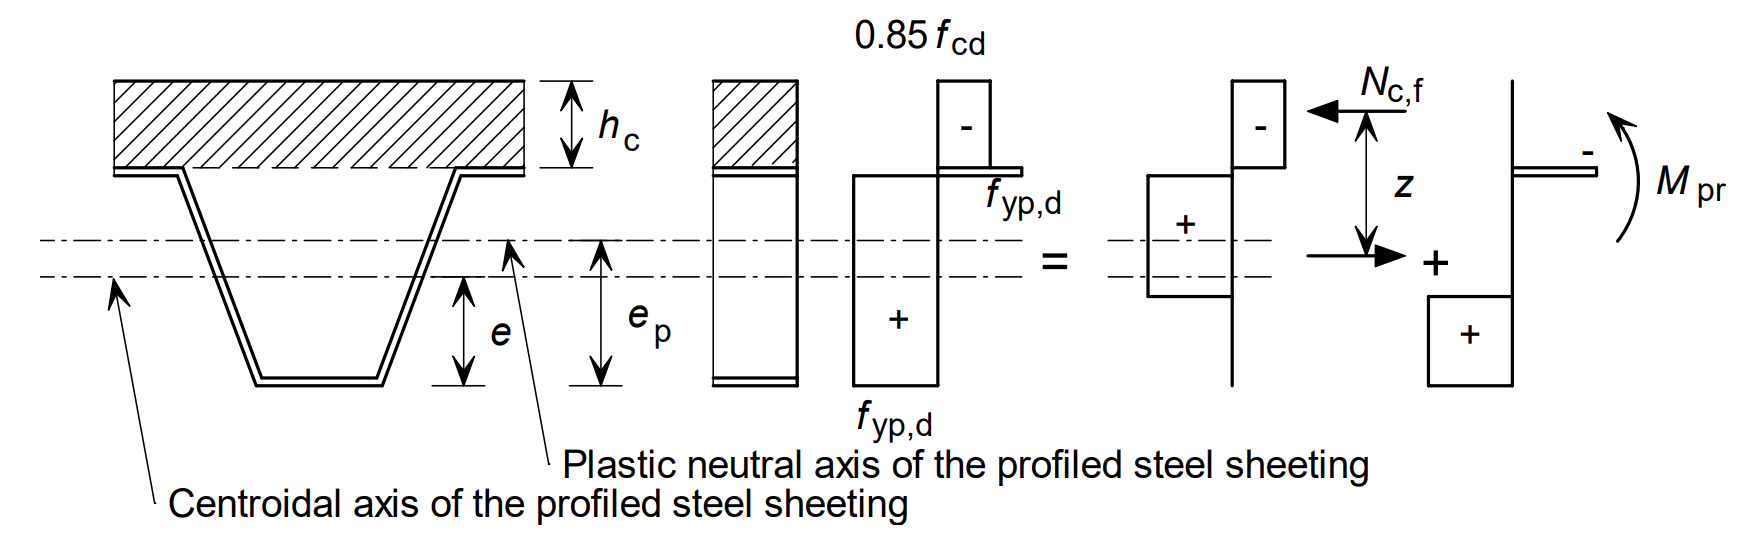
\includegraphics[width=\textwidth]{figures/saggingblockinsheeting.png}
        \caption{Sagging bending with the plastic neutral axis within the steel sheeting}
        \label{fig:stress_sagging_within}
    \end{subfigure}

    \vspace{1em}

    % --- (c) Hogging ---
    \begin{subfigure}[t]{0.9\textwidth}
        \centering
        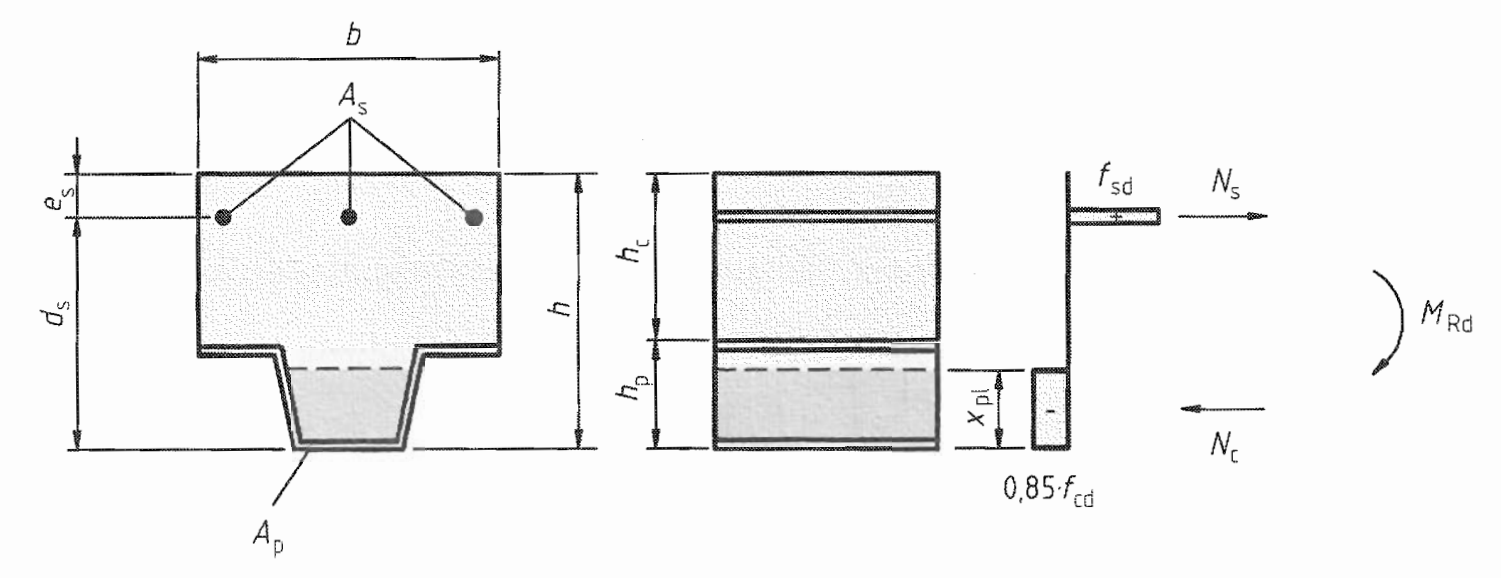
\includegraphics[width=\textwidth]{figures/hoggingblock.png}
        \caption{Hogging bending at an internal support}
        \label{fig:stress_hogging}
    \end{subfigure}

    \caption[Plastic stress distributions for composite slab bending]{Plastic stress distributions used for the ULS moment resistances, reproduced from EN~1994-1-1 Figures~9.5--9.7 \citep{RefWorks:cen2004en4}.}
    \label{fig:stress_blocks}
\end{figure}

\paragraph{Interaction of construction redistribution with composite hogging.}
The decision not to apply plastic redistribution at the construction stage (Section~\ref{sec:constr_stage}) has a consequence for the composite hogging resistance that is worth making explicit. 4-1-1/9.7.3(2)P permits the profiled steel sheeting to be included in the compression zone of the hogging cross-section only where the sheeting is continuous over the support \emph{and} no plastic redistribution of moments has been carried out at the construction stage. Because the present model treats the deck as simply supported during casting and therefore never applies construction-stage redistribution, this condition is always met for continuous configurations: the deck remains eligible to contribute to the composite hogging resistance, as reflected in Equation~\eqref{eq:hogging}. Had construction-stage redistribution been used, the deck would have to be excluded from the hogging calculation, reducing the available hogging resistance and requiring heavier support reinforcement. The simply-supported construction assumption is therefore not merely conservative at the construction stage but also slightly beneficial at the composite stage, since it preserves the deck contribution to hogging.

\paragraph{SLS deflection.}
The composite-stage deflection check uses the transformed composite second moment of area $I_c$, computed about the elastic neutral axis with concrete transformed to steel using the modular ratio $n$:
\begin{equation}
    I_c = \frac{b}{n} \cdot \frac{h_c^3}{12} + \frac{b\,h_c}{n}\left(\bar{y} - h_p - \frac{h_c}{2}\right)^2 + I_{p} + A_{p,e}\,(\bar{y} - e_p)^2
    \label{eq:Ic}
\end{equation}
The short-term modular ratio $n_0 = E_a/E_{cm}$ is used for variable loads; the long-term ratio $n_L = n_0(1 + 1.1\,\varphi_t)$ is used for permanent loads, with the creep coefficient $\varphi_t$ computed from 2-1-1 Annex B using the concrete mean strength $f_{cm} = f_{ck} + 8$\,MPa and the notional size $h_0 = 2\,h_c$. The notional size uses $h_0 = 2 h_c$ rather than $2 A_c / u$ since the steel deck seals the underside of the slab and only the top face is exposed to drying.

The treatment of self-weight deflection differs between propped and unpropped construction:

\begin{itemize}
    \item \textbf{Unpropped.} The deflection from deck self-weight and wet concrete is locked into the construction-stage deflected shape before composite action develops. This locked-in deflection has already been independently verified against $\delta_\mathrm{limit}$ per 4-1-1/9.3.2 (see above). The composite-stage $L/300$ total limit is therefore applied only to \emph{post-composite} deflections --- superimposed-dead load (SDL) and variable loads:
\begin{equation}
    \delta_\mathrm{tot} = \delta_\mathrm{SDL} + \delta_\mathrm{var} \le L/300
    \label{eq:delta_tot_unpropped}
\end{equation}

    \item \textbf{Propped.} Props carry the wet concrete weight during casting; on prop removal the composite section resists the full slab self-weight. The locked-in deflection is therefore zero, and the $L/300$ total limit applies to the sum of self-weight, SDL, and variable deflections --- all computed on the composite section:
\begin{equation}
    \delta_\mathrm{tot} = \delta_\mathrm{SW} + \delta_\mathrm{SDL} + \delta_\mathrm{var} \le L/300
    \label{eq:delta_tot_propped}
\end{equation}
\end{itemize}

In both cases, self-weight and SDL components use the long-term modular ratio $n_L$ to account for creep; the variable-load component uses $n_0$. An independent variable-load limit is also enforced:
\begin{equation}
    \delta_\mathrm{var} \le \min(L/350,\;20\,\mathrm{mm})
\end{equation}

\subsubsection*{Fire design}
\label{sec:fire}

Fire resistance is verified in accordance with 4-1-2 Annex~D, which provides a "model for the calculation of the fire resistance of unprotected composite slabs exposed to fire beneath the slab according to the standard temperature-time curve”. A default fire resistance period of R60 is applied. Four checks are performed in the following order.

\textbf{D1 --- Thermal insulation.} The insulation fire resistance time $t_i$ is calculated from formula D.1 as a function of the concrete depth above the ribs $h_c$, the upper-flange view factor $\Phi$ (formula D.3), the rib geometry factor $A/L_r$ (formula D.2), and the upper-flange width $l_3$, using the coefficient set of Table~D.1 for normal weight concrete:
\begin{equation}
    t_i = a_0 + a_1 h_c + a_2 \Phi + a_3 (A/L_r) + a_4 (1/l_3) + a_5 (A/L_r)(1/l_3)
    \label{eq:fire_d1}
\end{equation}
The check is satisfied when $t_i \ge R_\mathrm{fi}$.

\textbf{D4 --- Minimum effective thickness.} The effective slab thickness $h_\mathrm{eff}$ is computed from formulae D.15a or D.15b depending on the ratio $h_p/h_c$, and compared against the minimum values of Table~D.6. This check is independent of loading.

\textbf{D2 --- Sagging moment resistance.} The fire moment demand $M_\mathrm{Ed,fi}$ is calculated from the accidental load combination of EN~1990, using a fire combination factor $\psi_\mathrm{fi}$ that depends on occupancy. The deck steel temperature at the lower flange, web, and upper flange is calculated from formula D.4 (Table~D.2 coefficients):
\begin{equation}
    \theta_a = b_0 + b_1 (1/l_3) + b_2 (A/L_r) + b_3 \Phi + b_4 \Phi^2
    \label{eq:fire_d4}
\end{equation}
The corresponding strength reduction factor $k_{y,\theta}$ is obtained by linear interpolation through Table~3.2 of EN~1994-1-2. The sagging moment resistance at elevated temperature is then assembled from the deck contribution and the trough bar contribution using a rectangular stress block:
\begin{equation}
    M_\mathrm{Rd,fi} = N_\mathrm{deck,fi} \cdot z_\mathrm{deck} + N_\mathrm{bar,fi} \cdot z_\mathrm{bar}
    \label{eq:mrd_fi}
\end{equation}
where $N_\mathrm{deck,fi} = A_{p,e} \cdot f_{ypd} \cdot k_{y,\theta,\mathrm{deck}}$ and $N_\mathrm{bar,fi} = A_{s,\mathrm{tr}} \cdot f_{sk} \cdot k_{y,\theta,\mathrm{bar}}$.

Trough bar selection is carried out iteratively. Bar diameters of 8, 10, 12, 16, and 20\,mm are evaluated in ascending order. Each bar is assumed to be located at the geometric centre of the trough cross-section, with axis distances $u_1$ and $u_2$ derived from this central position; the axis distance $u_3$ from the lower flange is taken as 25\,mm for shallow profiles or 70\,mm for deep profiles. The temperature of each candidate bar is determined from formula D.5:
\begin{equation}
    \theta_s = c_0 + c_1 (u_3/h_p) + c_2 \sqrt{z} + c_3 (A/L_r) + c_4 \alpha + c_5 (1/l_3)
    \label{eq:fire_d5}
\end{equation}
where the position factor $z = 1/(1/\sqrt{u_1} + 1/\sqrt{u_2} + 1/\sqrt{u_3})$ and $\alpha$ is the web inclination. The smallest diameter for which $M_\mathrm{Rd,fi} \ge M_\mathrm{Ed,fi}$ is selected; if no diameter satisfies the check, the cross-section is recorded as failing D2.

\textbf{D3 --- Hogging moment at internal supports.} For continuous configurations only ($n_\mathrm{spans} > 1$), the reduced concrete compression zone depth due to isotherm penetration $b$ is determined by a single forward pass following the procedure of Annex~D.3: the limiting mesh temperature $\theta_\mathrm{lim}$ is obtained from formula D.7 (Table~D.4 coefficients), the position factor $z$ is inverted from formula D.5 using $u_3/h_p = 0.75$ (the value explicitly permitted by Annex~D.3 Note~6), and the isotherm penetration depth into the solid zone above the ribs is derived from formula D.11. The check is satisfied when the reduced-section hogging moment resistance $M_\mathrm{Rd,fi}$ equals or exceeds the fire hogging demand. The top mesh reinforcement on the unexposed face is assumed to remain at ambient temperature.

\subsubsection*{Vibration}
\label{sec:vibration_method}

Vibration serviceability is not incorporated as a structural constraint within the main optimisation. The Steel Construction Institute (SCI) publication 354 \citep{RefWorks:hicks2009p354} outlines the design guidance for all types of floor construction involving steel for determining the vibration response of sensitive floors. It is widely used in practice and allows the floor response to be compared with other UK documents such as BS 6472 and ISO 10137. The document was carried out as part of the ECSC project involving RWTH and Arcelor Profil Luxembourg Research.

The full method outlined in section 7 of this publication requires bay-level geometry inputs --- secondary beam span, primary beam span, bay width, and damping ratio --- none of which are defined in a slab-only optimisation study. Including a beam model would introduce multiple additional discrete variables (beam section, bay geometry) and fundamentally change the scope of the comparison, which is limited to the slab cross-section.
 
Instead, a slab-only screening check is performed as a post-processing step (implemented in \texttt{verify\_vibration.py}). The slab is modelled as a 1\,m-wide, simply-supported strip spanning the secondary-beam spacing $b$ on rigid supports, isolating the slab's own contribution to the floor frequency; this is the quantity reported by the ComFlor design tool, and it follows the SCI~P354 approach. The check proceeds in three steps.
 
First, the dynamic second moment of area of the slab strip is obtained from the power-law fit to SCI~P354 Table~7.2 for normal-weight concrete:
\begin{equation}
    I_s = c\, h_s^{3.7} \quad [\mathrm{mm^4/m}]
    \label{eq:vib_Is}
\end{equation}
where $h_s$ is the slab depth and $c$ is the Table~7.2 coefficient interpolated by rib height $h_p$ ($c = 0.37$ for re-entrant profiles; $c = 0.23$, $0.19$, and $0.05$ for trapezoidal profiles at $h_p \le 60$, $80$, and $225$\,mm respectively, linearly interpolated).
 
Second, the mid-span deflection of the simply-supported strip under the vibrating mass is computed:
\begin{equation}
    \delta = \frac{5\, m\, g\, b^4}{384\, EI_s} \quad [\mathrm{m}]
    \label{eq:vib_delta}
\end{equation}
where the floor mass per unit area is taken as the permanent load plus 10\% of the imposed load, with partitions excluded, in accordance with SCI~P354 4.1.2:
\begin{equation}
    m = \left(SW + \mathrm{SDL} + 0.1\, Q_k\right) \cdot 1000 / g \quad [\mathrm{kg/m^2}]
    \label{eq:vib_mass}
\end{equation}
The slab self-weight is computed consistently with the main optimiser from the profiled (average) concrete depth plus the deck sheeting. The superimposed and imposed loads match the office scenario, with $\mathrm{SDL} = 1.105$\,kN/m\textsuperscript{2} ($0.355$\,kN/m\textsuperscript{2} finishes $+\ 0.75$\,kN/m\textsuperscript{2} services) and $Q_k = 2.5$\,kN/m\textsuperscript{2}.
 
Third, the fundamental frequency is obtained from the resulting deflection using SCI~P354 Eq.~4:
\begin{equation}
    f_1 = \frac{18}{\sqrt{\delta_\mathrm{mm}}} \quad [\mathrm{Hz}]
    \label{eq:vib_f1}
\end{equation}
where $\delta_\mathrm{mm}$ is the mid-span deflection of Equation~\eqref{eq:vib_delta} expressed in millimetres. The slab is assessed against $f_1 \ge 3$\,Hz, the absolute SCI~P354 minimum for floor elements to avoid resonance due to walking.
 
This slab-only frequency is deliberately conservative as a screening check: the frequency of the complete floor, in which the slab is supported on flexible beams rather than rigid supports, is always \emph{lower} than the slab-alone value, because the beam flexibility adds to the total deflection. Passing the slab-only check is therefore necessary but not sufficient --- a floor that passes here may still fail once beam flexibility is included. The full system response-factor check, which accounts for beam and bay participation, modal mass, and damping, is implemented separately in \texttt{full\_vibration\_check.py}; a representative worked example of that full check is given in Appendix~\ref{app:vibration} to illustrate the procedure and to show the extent to which the full-floor frequency falls below the slab-alone screening value.
 
At longer office spans, vibration is likely to govern the overall composite floor design once beams are also considered. The implications are discussed further in Section~\ref{sec:assumptions}.

\todo[inline]{Add full bay configuration example to appendix.}

\subsubsection*{Acoustic performance}
\label{sec:acoustic}

Acoustic performance is not incorporated as a structural constraint within the optimisation. Instead, the floor build-up for each occupancy scenario (Table~\ref{tab:floor_buildup}) is pre-selected to meet the applicable acoustic requirements, and its GWP contribution is added to $\mathrm{GWP}_\mathrm{total}$ as described in Section~\ref{sec:env_impact}.

The two phenomena of concern are airborne sound transmission and impact sound transmission. In Switzerland, SIA~181 \citep{RefWorks:sia181} expresses its requirements using a standardised level difference $D_i$ for airborne sound and a standardised impact sound pressure level $L'_i$ for impact sound, set according to a classification of the sensitivity of the receiving space and the noise exposure.  In the United Kingdom, Approved Document~E \citep{RefWorks:adePartE} specifies field-measured requirements for separating floors for the standardised weighted sound level difference including a spectrum adaptation term ($D_{nT,w}+C_\mathrm{tr}$) and standrdised weighted impact sound preseure ($L'_{nT,w}$) levels. The requirements for each use case are given in Table~.

\todo[inline]{Add table of the requirements from word document 'acoustic checks'}

\todo[inline]{Explain method for making the floor build ups.}

The acoustic performance of each floor build up was estimated using the SCI publications 321 \citep{RefWorks:RefID:acousticslimdek} and 322 \citep{RefWorks:acousticcomposite}.

For the \textbf{office} scenario, the build-up consists of a raised access floor system comprising a chipboard panel (18\,mm), gypsum fibreboard (19\,mm), and rock wool insulation (30\,mm). Raised access floors are widely used in commercial office fit-out to route mechanical and electrical services and are compatible with composite slab construction without structural modifications.

For the \textbf{residential} scenario, the build-up comprises a two-layer factory-sealed parquet (11\,mm) over a cement screed (85\,mm) and glass wool insulation (30\,mm). For the \textbf{retail} scenario, a parquet finish over gypsum fibreboard and glass wool insulation is adopted. For the \textbf{industrial} scenario, a cement screed over rock wool insulation provides impact damping with minimal additional GWP. 

%===============================================================
\subsection{Environmental impact}
\label{sec:env_impact}
%===============================================================
The environmental impact of each cross-section is quantified as Global Warming Potential per metre of span length (kg\,CO$_2$-eq/m). The assessment covers EN~15804 modules A1--A3 (raw material supply, transport to factory, manufacturing) and modules C1--C4 (deconstruction, transport, waste processing, disposal). Modules A4--A5, B1--B7, and D are excluded as they introduce project-specific assumptions incompatible with early-stage comparative assessment.

The structural GWP is computed as the sum of four material contributions:
\begin{equation}
    \mathrm{GWP}_\mathrm{structure} = \rho_c \, h_\mathrm{c,avg} \, \mathrm{GWP}_c + \mathrm{GWP}_\mathrm{deck} + A_s \, \rho_s \, \mathrm{GWP}_s + A_{s,\mathrm{tr}} \, \rho_s \, \mathrm{GWP}_s
    \label{eq:gwp_structure}
\end{equation}

where $\rho_c$ and $\rho_s$ are the dry densities of concrete and reinforcing steel respectively; $A_s$ is the mesh cross-sectional area per unit width; $A_{s,\mathrm{tr}}$ is the trough bar area per unit width introduced by the fire check (zero if no trough bars are required); and $\mathrm{GWP}_c$, $\mathrm{GWP}_s$, and $\mathrm{GWP}_\mathrm{deck}$ are the GWP values drawn from the product database. The average concrete depth $h_\mathrm{c,avg}$ accounts for both the concrete above the ribs and the concrete that fills the trough voids:
\begin{equation}
    h_\mathrm{c,avg} = h_c + V_\mathrm{tr}
    \label{eq:hcavg}
\end{equation}
where $V_\mathrm{tr}$ is the trough concrete volume per unit plan area (m$^3$/m$^2$), sourced from the manufacturer database.

The deck contribution $\mathrm{GWP}_\mathrm{deck}$ is normalised to a per-metre-length basis before summation. Where the manufacturer EPD is expressed per unit area, the value is multiplied by the unit strip width of 1\,m. Where the EPD is expressed per unit mass, the value is converted using the manufacturer-declared deck weight per unit area:
\begin{equation}
    \mathrm{GWP}_\mathrm{deck} = 
    \begin{cases}
    \mathrm{GWP}_\mathrm{deck}^{(\mathrm{m}^2)} \cdot b           & \text{if EPD per m}^2 \\
    w_\mathrm{deck} \cdot \mathrm{GWP}_\mathrm{deck}^{(\mathrm{kg})} \cdot b & \text{if EPD per kg or per t}
    \end{cases}
    \label{eq:gwp_deck_norm}
\end{equation}
where $w_\mathrm{deck}$ is the deck weight in kg/m$^2$ and $b = 1$\,m is the strip width.

The total GWP is obtained by adding the contribution of the non-structural floor build-up to the structural cross-section:
\begin{equation}
    \mathrm{GWP}_\mathrm{total} = \mathrm{GWP}_\mathrm{structure} + \sum_{i \in \mathrm{layers}} \rho_i \, t_i \, \mathrm{GWP}_i
    \label{eq:gwp_total}
\end{equation}
where the sum runs over all layers in the floor build-up table for the relevant occupancy scenario (Table~\ref{tab:floor_buildup}), and $\rho_i$, $t_i$, $\mathrm{GWP}_i$ are the layer density, thickness, and GWP value respectively.

%===============================================================
\subsection{Optimisation}
\label{sec:optimisation}
%===============================================================
The optimisation of composite slab cross-sections differs from the approach used for the reinforced concrete and timber baselines in the pre-existing framework. Because the composite slab has a single continuous design variable --- the total slab depth $h$ --- a scalar bounded optimisation is both sufficient and substantially more efficient than the multi-variable basin-hopping approach used for the RC and timber classes. The complete workflow is shown in Figure~\ref{fig:code_flowchart}, in which the boxes are coloured by the source module responsible for each stage.

\begin{figure}[p]
  \centering
  \resizebox{\textwidth}{!}{% ============================================================================
%  Composite slab optimisation workflow — flowchart for the Methodology chapter
%  Boxes are colour-coded by source module; each box is tagged with the
%  script and the class / function used at that stage.
%
%  Requires in MAIN.tex preamble:
%     \usepackage{tikz}
%     \usetikzlibrary{shapes.geometric, arrows.meta, positioning, calc, fit, backgrounds}
%  Then include with:  % ============================================================================
%  Composite slab optimisation workflow — flowchart for the Methodology chapter
%  Boxes are colour-coded by source module; each box is tagged with the
%  script and the class / function used at that stage.
%
%  Requires in MAIN.tex preamble:
%     \usepackage{tikz}
%     \usetikzlibrary{shapes.geometric, arrows.meta, positioning, calc, fit, backgrounds}
%  Then include with:  \input{code_flowchart}   (inside a figure environment)
% ============================================================================
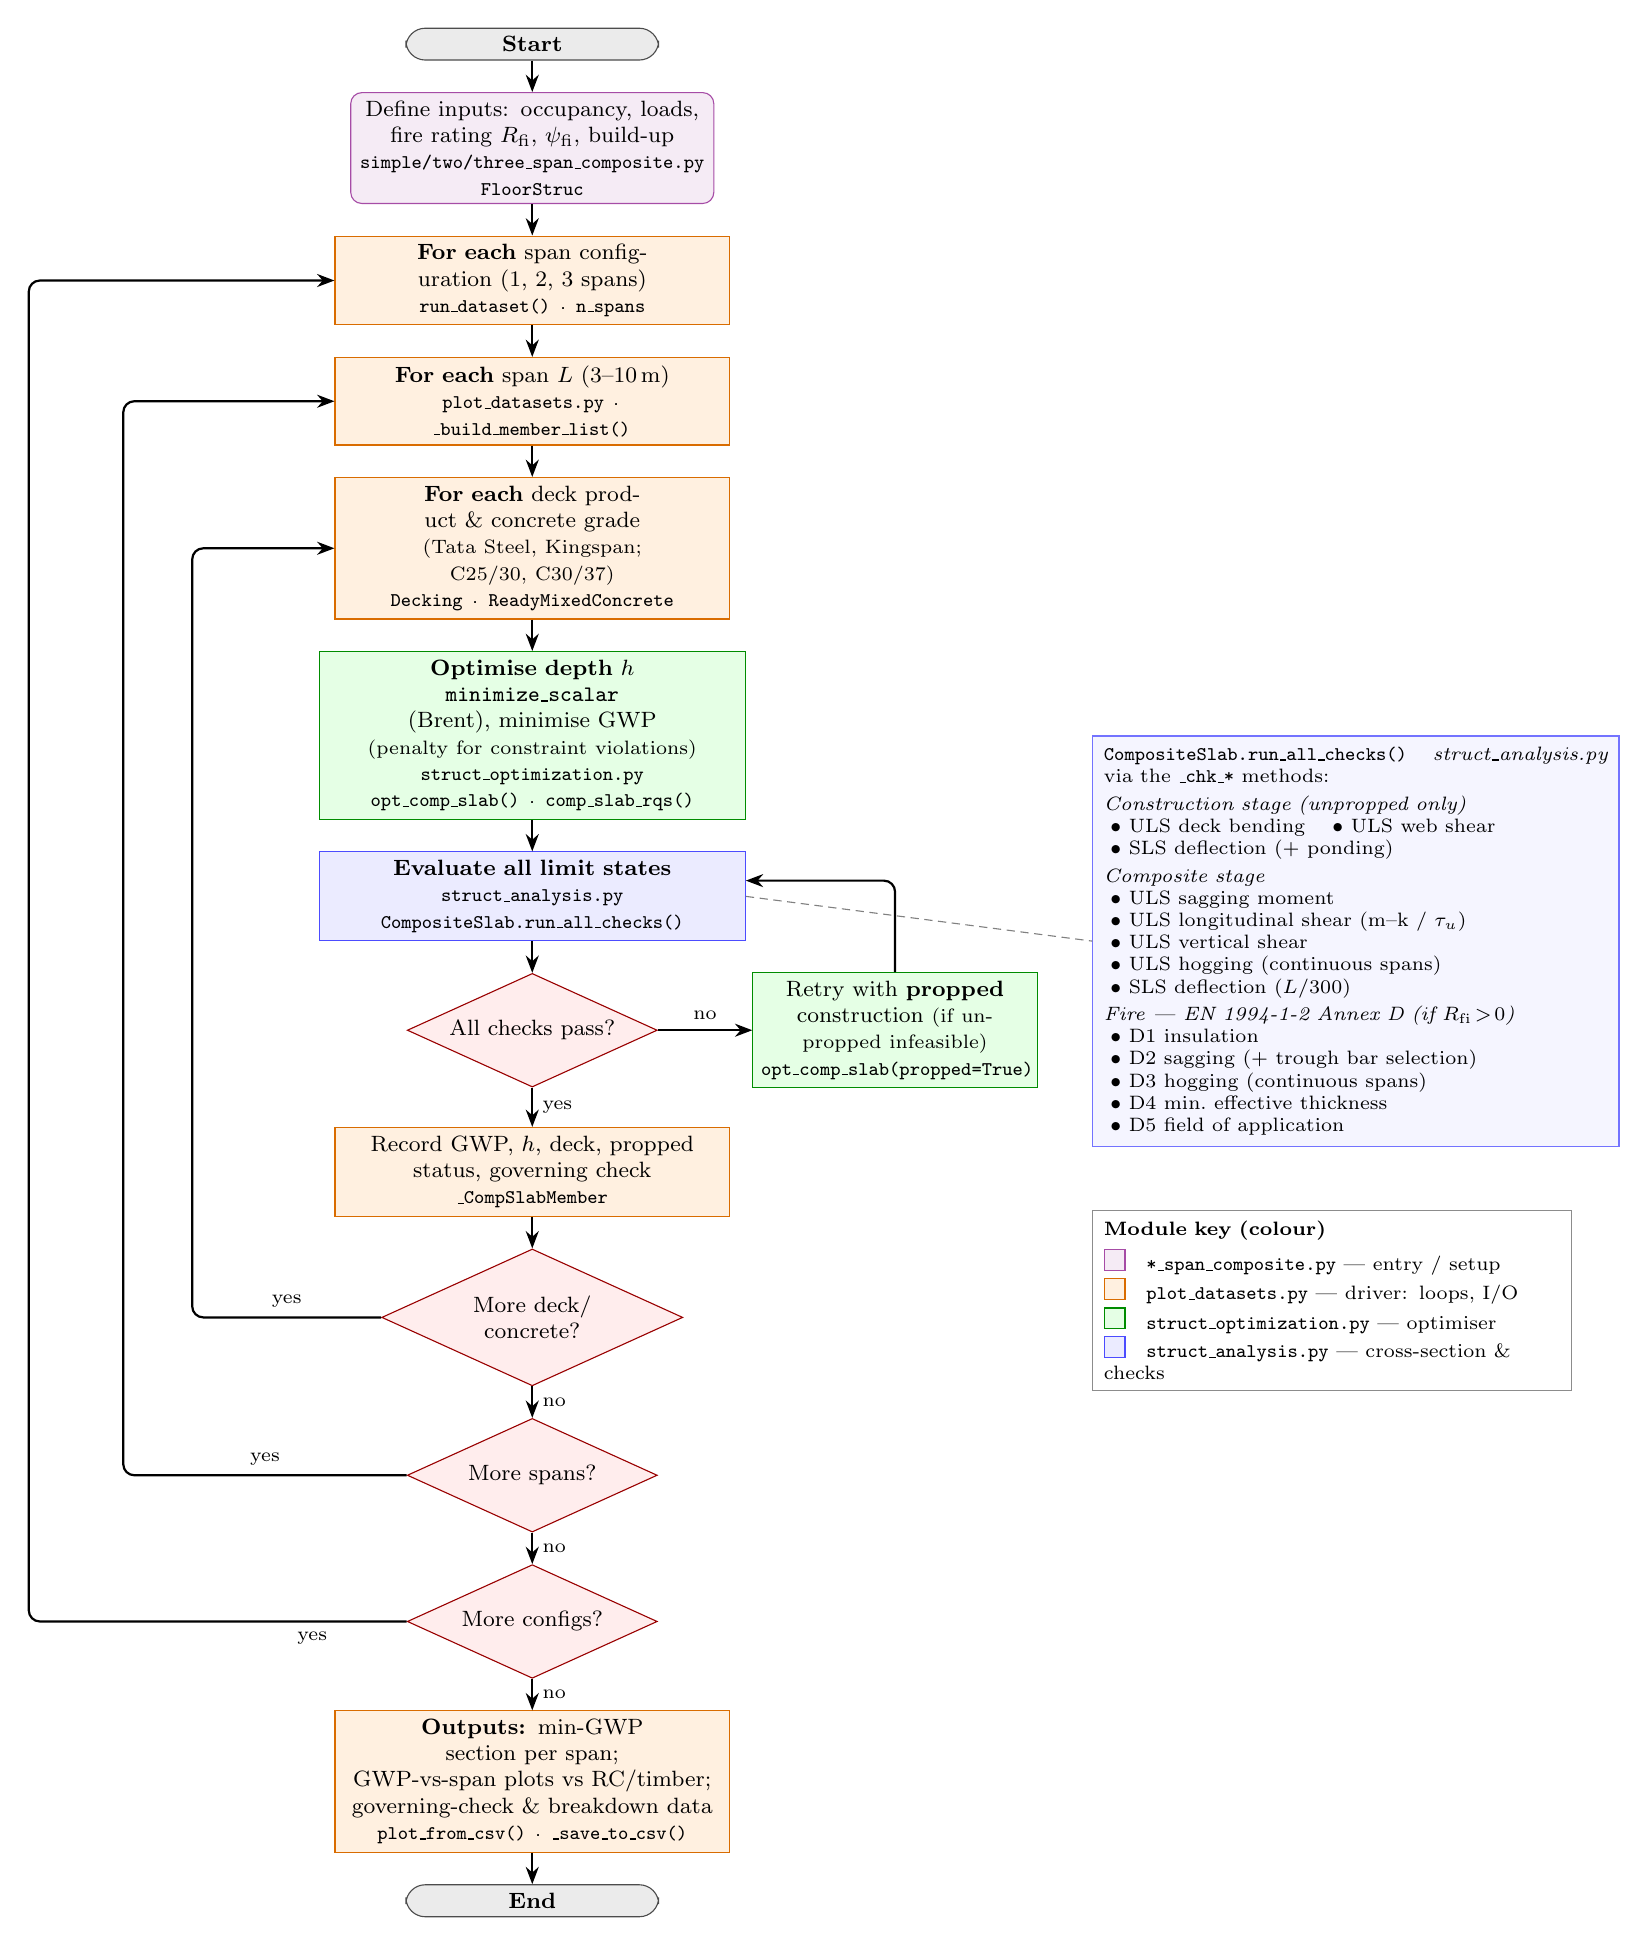
\begin{tikzpicture}[
    font=\footnotesize,
    node distance = 4mm and 10mm,
    >={Stealth[length=2.2mm]},
    line/.style   = {draw, ->, thick, rounded corners},
    % --- module colours ---
    entry/.style  = {rectangle, rounded corners=4pt, draw=violet!70, fill=violet!8,
                     text width=44mm, align=center, inner sep=3pt},
    driver/.style = {rectangle, draw=orange!85!black, fill=orange!12,
                     text width=48mm, align=center, inner sep=3pt},
    optim/.style  = {rectangle, draw=green!55!black, fill=green!10,
                     text width=52mm, align=center, inner sep=3pt},
    analysis/.style = {rectangle, draw=blue!70, fill=blue!8,
                     text width=52mm, align=center, inner sep=3pt},
    startstop/.style = {rectangle, rounded corners=7pt, draw=black!70, fill=black!8,
                     text width=30mm, align=center, inner sep=3pt},
    decision/.style = {diamond, aspect=2.2, draw=red!60!black, fill=red!7,
                     text width=24mm, align=center, inner sep=1pt},
    check/.style  = {rectangle, draw=blue!55, fill=blue!4, text width=64mm,
                     align=left, inner sep=4pt, font=\scriptsize},
]

% ---- main vertical spine -------------------------------------------------
\node[startstop] (start) {\textbf{Start}};

\node[entry, below=of start] (inputs)
   {Define inputs: occupancy, loads,\\ fire rating $R_\mathrm{fi}$, $\psi_\mathrm{fi}$, build-up\\
    {\ttfamily\scriptsize simple/two/three\_span\_composite.py}\\ {\ttfamily\scriptsize FloorStruc}};

\node[driver, below=of inputs] (cfg)
   {\textbf{For each} span configuration (1, 2, 3 spans)\\
    {\ttfamily\scriptsize run\_dataset() · n\_spans}};

\node[driver, below=of cfg] (span)
   {\textbf{For each} span $L$ (3--10\,m)\\
    {\ttfamily\scriptsize plot\_datasets.py · \_build\_member\_list()}};

\node[driver, below=of span] (deck)
   {\textbf{For each} deck product \& concrete grade\\ {\scriptsize(Tata Steel, Kingspan; C25/30, C30/37)}\\
    {\ttfamily\scriptsize Decking · ReadyMixedConcrete}};

\node[optim, below=of deck] (opt)
   {\textbf{Optimise depth $h$}\\ \texttt{minimize\_scalar} (Brent), minimise GWP\\ {\scriptsize(penalty for constraint violations)}\\
    {\ttfamily\scriptsize struct\_optimization.py}\\ {\ttfamily\scriptsize opt\_comp\_slab() · comp\_slab\_rqs()}};

\node[analysis, below=of opt] (checks)
   {\textbf{Evaluate all limit states}\\
    {\ttfamily\scriptsize struct\_analysis.py}\\ {\ttfamily\scriptsize CompositeSlab.run\_all\_checks()}};

\node[decision, below=of checks] (feas) {All checks pass?};

\node[driver, below=5mm of feas] (record)
   {Record GWP, $h$, deck, propped status, governing check\\
    {\ttfamily\scriptsize \_CompSlabMember}};

\node[decision, below=of record]   (moredeck) {More deck/\\ concrete?};
\node[decision, below=of moredeck]  (morespan) {More spans?};
\node[decision, below=of morespan]  (morecfg)  {More configs?};

\node[driver, below=of morecfg] (out)
   {\textbf{Outputs:} min-GWP section per span;\\ GWP-vs-span plots vs RC/timber;\\ governing-check \& breakdown data\\
    {\ttfamily\scriptsize plot\_from\_csv() · \_save\_to\_csv()}};

\node[startstop, below=of out] (stop) {\textbf{End}};

% ---- spine arrows --------------------------------------------------------
\draw[line] (start) -- (inputs);
\draw[line] (inputs) -- (cfg);
\draw[line] (cfg) -- (span);
\draw[line] (span) -- (deck);
\draw[line] (deck) -- (opt);
\draw[line] (opt) -- (checks);
\draw[line] (checks) -- (feas);
\draw[line] (feas) -- node[right, font=\scriptsize] {yes} (record);
\draw[line] (record) -- (moredeck);
\draw[line] (moredeck) -- node[right, font=\scriptsize] {no} (morespan);
\draw[line] (morespan) -- node[right, font=\scriptsize] {no} (morecfg);
\draw[line] (morecfg) -- node[right, font=\scriptsize] {no} (out);
\draw[line] (out) -- (stop);

% ---- feasibility "no" -> propped retry -----------------------------------
\node[optim, right=12mm of feas, text width=34mm] (propped)
   {Retry with \textbf{propped} construction {\scriptsize(if unpropped infeasible)}\\
    {\ttfamily\scriptsize opt\_comp\_slab(propped=True)}};
\draw[line] (feas.east) -- node[above, font=\scriptsize] {no} (propped.west);
\draw[line] (propped.north) |- ($(checks.east)+(0,2mm)$);

% ---- loop-back arrows ----------------------------------------------------
\draw[line] (moredeck.west) -- node[above, font=\scriptsize] {yes} ++(-24mm,0) |- (deck.west);
\draw[line] (morespan.west) -- node[above, font=\scriptsize] {yes} ++(-36mm,0) |- (span.west);
\draw[line] (morecfg.west)  -- node[below, font=\scriptsize, pos=0.25] {yes} ++(-48mm,0) |- (cfg.west);

% ---- run_all_checks expansion (right callout) ----------------------------
\node[check, right=44mm of opt, anchor=north west] (cklist)
  {\textbf{\texttt{CompositeSlab.run\_all\_checks()}} \hfill {\scriptsize\itshape struct\_analysis.py}\\
   {\scriptsize via the \texttt{\_chk\_*} methods:}\\[2pt]
   \textit{Construction stage (unpropped only)}\\
   \;$\bullet$ ULS deck bending \;\; $\bullet$ ULS web shear\\
   \;$\bullet$ SLS deflection (+ ponding)\\[2pt]
   \textit{Composite stage}\\
   \;$\bullet$ ULS sagging moment\\
   \;$\bullet$ ULS longitudinal shear (m--k / $\tau_u$)\\
   \;$\bullet$ ULS vertical shear\\
   \;$\bullet$ ULS hogging (continuous spans)\\
   \;$\bullet$ SLS deflection ($L/300$)\\[2pt]
   \textit{Fire — EN 1994-1-2 Annex D (if $R_\mathrm{fi}\!>\!0$)}\\
   \;$\bullet$ D1 insulation\\
   \;$\bullet$ D2 sagging (+ trough bar selection)\\
   \;$\bullet$ D3 hogging (continuous spans)\\
   \;$\bullet$ D4 min.\ effective thickness\\
   \;$\bullet$ D5 field of application};
\draw[densely dashed, gray] (checks.east) -- (cklist.west);

% ---- module legend (bottom-right) ----------------------------------------
\node[check, draw=black!45, fill=white, text width=58mm, below=8mm of cklist.south west, anchor=north west] (legend)
  {\textbf{Module key (colour)}\\[2pt]
   \tikz\fill[violet!8,draw=violet!70](0,0)rectangle(2.6mm,2.6mm); \; \texttt{*\_span\_composite.py} — entry / setup\\
   \tikz\fill[orange!12,draw=orange!85!black](0,0)rectangle(2.6mm,2.6mm); \; \texttt{plot\_datasets.py} — driver: loops, I/O\\
   \tikz\fill[green!10,draw=green!55!black](0,0)rectangle(2.6mm,2.6mm); \; \texttt{struct\_optimization.py} — optimiser\\
   \tikz\fill[blue!8,draw=blue!70](0,0)rectangle(2.6mm,2.6mm); \; \texttt{struct\_analysis.py} — cross-section \& checks};

\end{tikzpicture}
   (inside a figure environment)
% ============================================================================
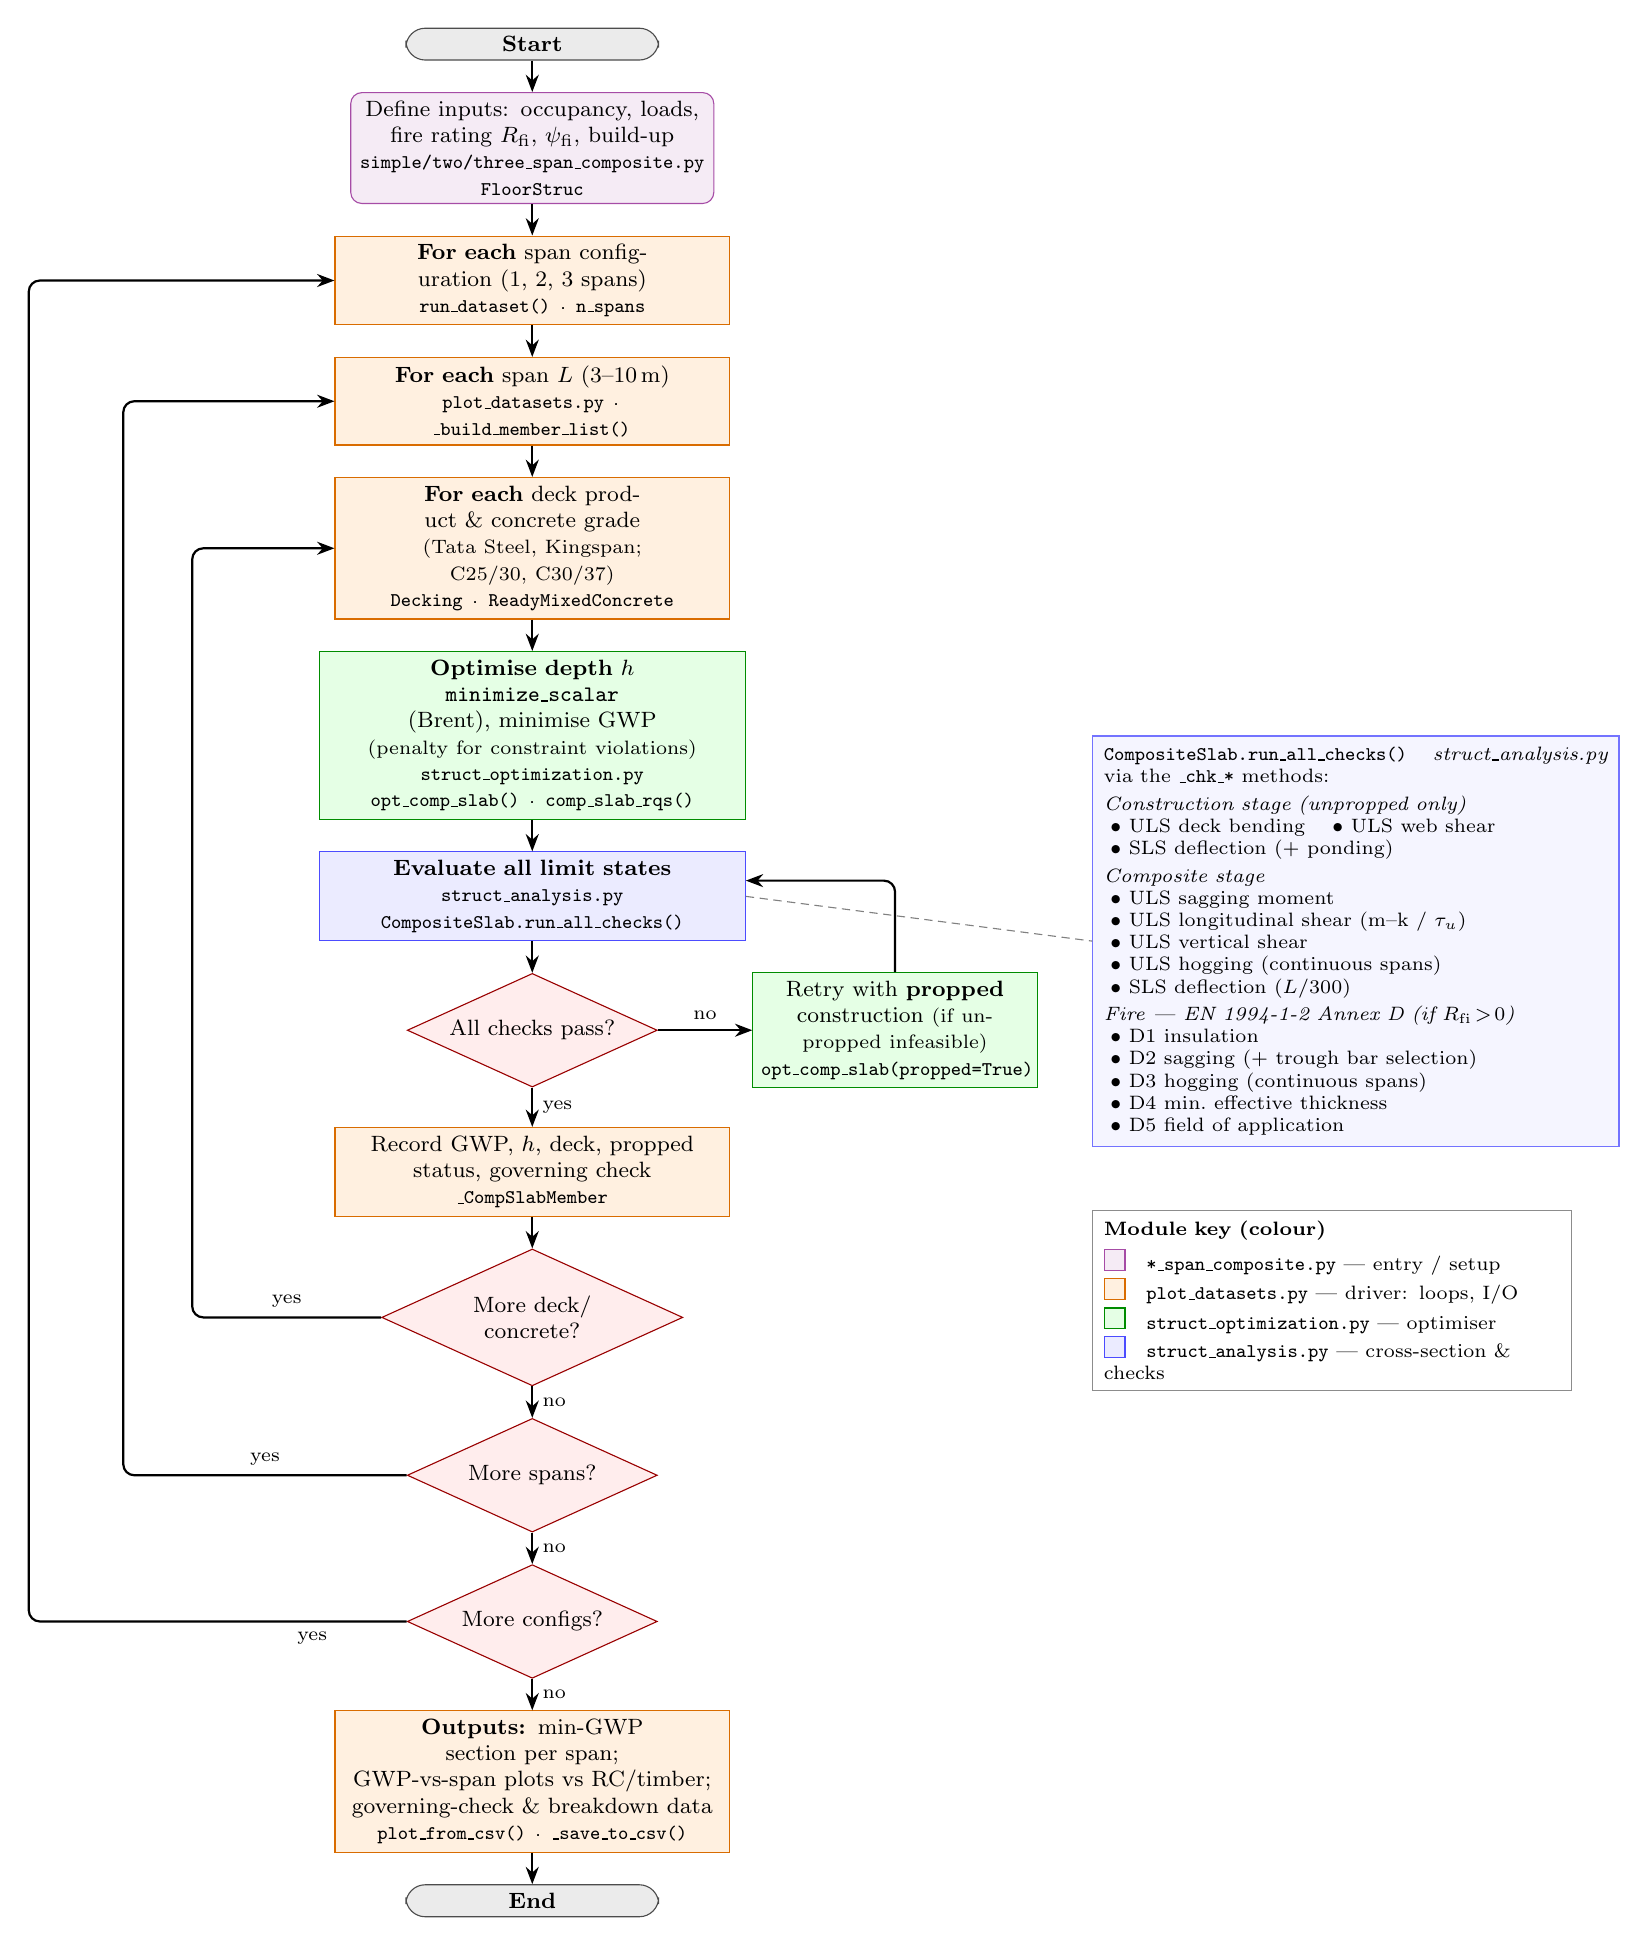
\begin{tikzpicture}[
    font=\footnotesize,
    node distance = 4mm and 10mm,
    >={Stealth[length=2.2mm]},
    line/.style   = {draw, ->, thick, rounded corners},
    % --- module colours ---
    entry/.style  = {rectangle, rounded corners=4pt, draw=violet!70, fill=violet!8,
                     text width=44mm, align=center, inner sep=3pt},
    driver/.style = {rectangle, draw=orange!85!black, fill=orange!12,
                     text width=48mm, align=center, inner sep=3pt},
    optim/.style  = {rectangle, draw=green!55!black, fill=green!10,
                     text width=52mm, align=center, inner sep=3pt},
    analysis/.style = {rectangle, draw=blue!70, fill=blue!8,
                     text width=52mm, align=center, inner sep=3pt},
    startstop/.style = {rectangle, rounded corners=7pt, draw=black!70, fill=black!8,
                     text width=30mm, align=center, inner sep=3pt},
    decision/.style = {diamond, aspect=2.2, draw=red!60!black, fill=red!7,
                     text width=24mm, align=center, inner sep=1pt},
    check/.style  = {rectangle, draw=blue!55, fill=blue!4, text width=64mm,
                     align=left, inner sep=4pt, font=\scriptsize},
]

% ---- main vertical spine -------------------------------------------------
\node[startstop] (start) {\textbf{Start}};

\node[entry, below=of start] (inputs)
   {Define inputs: occupancy, loads,\\ fire rating $R_\mathrm{fi}$, $\psi_\mathrm{fi}$, build-up\\
    {\ttfamily\scriptsize simple/two/three\_span\_composite.py}\\ {\ttfamily\scriptsize FloorStruc}};

\node[driver, below=of inputs] (cfg)
   {\textbf{For each} span configuration (1, 2, 3 spans)\\
    {\ttfamily\scriptsize run\_dataset() · n\_spans}};

\node[driver, below=of cfg] (span)
   {\textbf{For each} span $L$ (3--10\,m)\\
    {\ttfamily\scriptsize plot\_datasets.py · \_build\_member\_list()}};

\node[driver, below=of span] (deck)
   {\textbf{For each} deck product \& concrete grade\\ {\scriptsize(Tata Steel, Kingspan; C25/30, C30/37)}\\
    {\ttfamily\scriptsize Decking · ReadyMixedConcrete}};

\node[optim, below=of deck] (opt)
   {\textbf{Optimise depth $h$}\\ \texttt{minimize\_scalar} (Brent), minimise GWP\\ {\scriptsize(penalty for constraint violations)}\\
    {\ttfamily\scriptsize struct\_optimization.py}\\ {\ttfamily\scriptsize opt\_comp\_slab() · comp\_slab\_rqs()}};

\node[analysis, below=of opt] (checks)
   {\textbf{Evaluate all limit states}\\
    {\ttfamily\scriptsize struct\_analysis.py}\\ {\ttfamily\scriptsize CompositeSlab.run\_all\_checks()}};

\node[decision, below=of checks] (feas) {All checks pass?};

\node[driver, below=5mm of feas] (record)
   {Record GWP, $h$, deck, propped status, governing check\\
    {\ttfamily\scriptsize \_CompSlabMember}};

\node[decision, below=of record]   (moredeck) {More deck/\\ concrete?};
\node[decision, below=of moredeck]  (morespan) {More spans?};
\node[decision, below=of morespan]  (morecfg)  {More configs?};

\node[driver, below=of morecfg] (out)
   {\textbf{Outputs:} min-GWP section per span;\\ GWP-vs-span plots vs RC/timber;\\ governing-check \& breakdown data\\
    {\ttfamily\scriptsize plot\_from\_csv() · \_save\_to\_csv()}};

\node[startstop, below=of out] (stop) {\textbf{End}};

% ---- spine arrows --------------------------------------------------------
\draw[line] (start) -- (inputs);
\draw[line] (inputs) -- (cfg);
\draw[line] (cfg) -- (span);
\draw[line] (span) -- (deck);
\draw[line] (deck) -- (opt);
\draw[line] (opt) -- (checks);
\draw[line] (checks) -- (feas);
\draw[line] (feas) -- node[right, font=\scriptsize] {yes} (record);
\draw[line] (record) -- (moredeck);
\draw[line] (moredeck) -- node[right, font=\scriptsize] {no} (morespan);
\draw[line] (morespan) -- node[right, font=\scriptsize] {no} (morecfg);
\draw[line] (morecfg) -- node[right, font=\scriptsize] {no} (out);
\draw[line] (out) -- (stop);

% ---- feasibility "no" -> propped retry -----------------------------------
\node[optim, right=12mm of feas, text width=34mm] (propped)
   {Retry with \textbf{propped} construction {\scriptsize(if unpropped infeasible)}\\
    {\ttfamily\scriptsize opt\_comp\_slab(propped=True)}};
\draw[line] (feas.east) -- node[above, font=\scriptsize] {no} (propped.west);
\draw[line] (propped.north) |- ($(checks.east)+(0,2mm)$);

% ---- loop-back arrows ----------------------------------------------------
\draw[line] (moredeck.west) -- node[above, font=\scriptsize] {yes} ++(-24mm,0) |- (deck.west);
\draw[line] (morespan.west) -- node[above, font=\scriptsize] {yes} ++(-36mm,0) |- (span.west);
\draw[line] (morecfg.west)  -- node[below, font=\scriptsize, pos=0.25] {yes} ++(-48mm,0) |- (cfg.west);

% ---- run_all_checks expansion (right callout) ----------------------------
\node[check, right=44mm of opt, anchor=north west] (cklist)
  {\textbf{\texttt{CompositeSlab.run\_all\_checks()}} \hfill {\scriptsize\itshape struct\_analysis.py}\\
   {\scriptsize via the \texttt{\_chk\_*} methods:}\\[2pt]
   \textit{Construction stage (unpropped only)}\\
   \;$\bullet$ ULS deck bending \;\; $\bullet$ ULS web shear\\
   \;$\bullet$ SLS deflection (+ ponding)\\[2pt]
   \textit{Composite stage}\\
   \;$\bullet$ ULS sagging moment\\
   \;$\bullet$ ULS longitudinal shear (m--k / $\tau_u$)\\
   \;$\bullet$ ULS vertical shear\\
   \;$\bullet$ ULS hogging (continuous spans)\\
   \;$\bullet$ SLS deflection ($L/300$)\\[2pt]
   \textit{Fire — EN 1994-1-2 Annex D (if $R_\mathrm{fi}\!>\!0$)}\\
   \;$\bullet$ D1 insulation\\
   \;$\bullet$ D2 sagging (+ trough bar selection)\\
   \;$\bullet$ D3 hogging (continuous spans)\\
   \;$\bullet$ D4 min.\ effective thickness\\
   \;$\bullet$ D5 field of application};
\draw[densely dashed, gray] (checks.east) -- (cklist.west);

% ---- module legend (bottom-right) ----------------------------------------
\node[check, draw=black!45, fill=white, text width=58mm, below=8mm of cklist.south west, anchor=north west] (legend)
  {\textbf{Module key (colour)}\\[2pt]
   \tikz\fill[violet!8,draw=violet!70](0,0)rectangle(2.6mm,2.6mm); \; \texttt{*\_span\_composite.py} — entry / setup\\
   \tikz\fill[orange!12,draw=orange!85!black](0,0)rectangle(2.6mm,2.6mm); \; \texttt{plot\_datasets.py} — driver: loops, I/O\\
   \tikz\fill[green!10,draw=green!55!black](0,0)rectangle(2.6mm,2.6mm); \; \texttt{struct\_optimization.py} — optimiser\\
   \tikz\fill[blue!8,draw=blue!70](0,0)rectangle(2.6mm,2.6mm); \; \texttt{struct\_analysis.py} — cross-section \& checks};

\end{tikzpicture}
}
  \caption{Workflow of the composite slab optimisation. Boxes are coloured by the source module responsible for each stage (see key), and each box is tagged with the relevant script and class or function.}
  \label{fig:code_flowchart}
\end{figure}

\subsubsection*{Composite slab: Brent's bounded method}
For the \texttt{CompositeSlab} class, the function \texttt{opt\_comp\_slab} in \texttt{struct\_optimization.py} minimises the objective function over the single continuous variable $h \in [h_\mathrm{min},\, 500\,\mathrm{mm}]$ using \texttt{scipy.optimize.minimize\_scalar} with the \texttt{bounded} (Brent) method. Brent's method is a bracketed root-finding and minimum-finding algorithm that combines golden-section search with parabolic interpolation; for a smooth, unimodal objective function, it converges in approximately 15--20 function evaluations, compared with 200+ evaluations required by the basin-hopping procedure used for the other slab typologies. The tolerance is set to $0.5$\,mm in $h$, which is small relative to the discrete step size implicit in the discrete variables (deck product, concrete grade) and has negligible influence on the reported GWP.

The objective function is the structural GWP of the cross-section per Equation~\eqref{eq:gwp_structure}. Structural constraints are incorporated via a penalty function: the objective is multiplied by a factor $(1 + \Pi)$, where $\Pi$ is the sum of constraint violation penalties proportional to the degree of each violation, with large penalty coefficients (of order $10^5$) applied to ensure that infeasible cross-sections are strongly discouraged. The combined feasibility criterion (\texttt{ENV} in the implementation) requires simultaneous satisfaction of all construction-stage and composite-stage limit states together with the applicable fire checks.

The outer optimisation loop iterates over all combinations of deck product and concrete grade in the database. The global minimum across all discrete combinations is taken as the optimal design for that span. Propping is handled at the outer loop level: an unpropped optimisation is first attempted, and if no feasible solution is found (i.e.\ the optimal section still fails at least one check at $h = 500$\,mm), a propped optimisation is run for the same (deck, concrete grade) combination. The propped/unpropped status of the final result is recorded and reported alongside the optimal GWP and cross-section geometry.\todo[inline]{check the logic for propped construction, may need to change flowchart and explanation}

The RC rectangular slab, RC ribbed slab, and timber cross-sections are optimised using the basin-hopping algorithm from the SciPy optimisation library \citep{RefWorks:wales1997global}, which combines a global stochastic search with a local Powell minimiser. These cross-sections have multiple continuous variables (height, reinforcement diameter) for which a multi-variable global search is appropriate. The composite slab, with its single continuous variable and large outer enumeration over discrete deck--concrete combinations, does not benefit from this approach and converges reliably with the bounded scalar method.

%===============================================================
\subsection{Validation of structural model}
\label{sec:validation}
%===============================================================
To verify the correct implementation of the design procedures, the structural model was compared against published manufacturer design tables for representative deck products and span configurations. Manufacturer design tables are derived from structural test results and detailed calculations and therefore provide an independent reference against which the implementation can be assessed.

For each validation case, the model-computed maximum permissible span at a given slab depth was compared against the corresponding manufacturer-tabulated value for the same loading and fire rating. Validation was performed across the following deck families: ComFlor~225 and ComFlor~51/60/80 (Tata Steel, EC~4 design tables), ComFlor~210 (Tata Steel, BS~5950 design tables), and Multideck~60/80/146 (Kingspan, BS~5950 design tables). 

%===============================================================
\subsection{Assumptions and limitations}
\label{sec:assumptions}
%===============================================================
The methodology described above relies on a number of simplifying assumptions, summarised in this section together with their justifications. The assumptions are grouped by category to clarify their scope and the extent to which they affect the comparative results.

\subsubsection*{Structural modelling assumptions}

\paragraph{Linear elastic, uncracked behaviour for serviceability deflection.}
SLS deflections are computed using the linear-elastic uncracked transformed section per 4-1-1/9.8.2(7). Tension stiffening and partial cracking are not modelled. This assumption is consistent with the simplified deflection method permitted by EN~1994-1-1 for unpropped composite slabs and is widely used in industry practice \citep{RefWorks:scip359}.

\paragraph{Effective deck area $A_{p,e}$ fallback.}
The effective cross-sectional area $A_{p,e}$ accounts for local buckling reductions in the deck profile under bending and is normally derived from manufacturer test data. Where the manufacturer technical manual does not publish $A_{p,e}$ explicitly, a conservative fallback is applied: $A_{p,e} = 0.9\,A_p$ for shallow profiles ($h_p < 80$\,mm) and $A_{p,e} = 0.5\,A_p$ for deep profiles ($h_p \ge 80$\,mm) - derived from calculating the average reduction in area from manufacturer data. This fallback affects the computed sagging moment resistance and longitudinal shear resistance and introduces a conservative bias relative to manufacturer software where the test-derived $A_{p,e}$ is used directly.

\paragraph{Vibration check: slab-only, beams excluded.}
As discussed in Section~\ref{sec:vibration_method}, the vibration check is performed on the isolated slab strip and omits beam participation. For office spans of 6\,m and above, the slab-alone natural frequency may decrease and approach the 3\,Hz threshold, and the full composite floor system --- including beam depth, bay width, and damping --- may govern the SLS design when evaluated per SCI~P354. The implication is that the optimal composite slab depths reported for office occupancy at longer spans may need to be increased if the full vibration check is applied, which would increase the reported GWP. The comparative ranking between slab systems may therefore be more favourable to RC flat slabs at longer office spans than the optimisation results suggest, since RC slabs benefit from higher mass (and consequently lower vibration acceleration response) at the same slab depth.

\subsubsection*{Construction-related assumptions}

\paragraph{Deck continuity over intermediate supports.}
For multi-span configurations, the steel deck is assumed to be continuous (lapped) over intermediate supports, in accordance with standard construction practice and SCI~P300 \citep{RefWorks:scip300}. Construction-stage moment coefficients are taken from elastic analysis.

\paragraph{Local resistance checks (construction stage) not implemented.}
Local resistance checks at supports per EN~1993-1-3 Cl.\,6.1.7 (web crippling and combined bending plus support reaction) are not currently implemented. These checks are not expected to control for the span and load ranges considered.

\subsubsection*{Material and EPD assumptions}

\paragraph{Concrete grade range C25/30 to C30/37.}
Only normal-weight concrete grades C25/30 and C30/37 are considered, as increased compressive strength provides limited benefit for the composite slab configurations at the spans considered and the EPD intensity per kg increases with strength grade. C20/25 is excluded in order to align with industry practice outlined by the technical manuals which all assume either C25/30 or C30/37 - see Section BLANK for further discussion.
\todo[inline]{add reference to section later on which discusses effect of running with C20 as it seems to work structurally even if its not industry practice}

\paragraph{Granularity of deck EPDs.}
Tata Steel publish individual EPDs for each ComFlor profile and gauge combination. Kingspan publish a single EPD per tonne of steel for the entire Multideck range. ArcelorMittal Cofraplus and Cofrastra products are included in the database but are excluded from the main optimisation runs: ArcelorMittal publish a single EPD covering all deck profiles regardless of depth or gauge, which does not reflect the substantially different steel quantities per unit area between shallow and deep profiles. After comparing individual manufacturer EPDs with the KBOB reference database, it was determined that the ArcelorMittal single-EPD approach would severely underrepresent the GWP of all decking profiles, introducing a systematic bias that would distort the comparative results. Tata Steel and Kingspan products are therefore retained as the primary optimisation dataset. The KBOB GWP value for coated flat steel is 3.64 kg co2eq/kg steel, ComFlor's EPDs provide a GWP of between 2.83 and 3.09, Mutlideck has a value of 2.50 while Arcelor Mittal's EPD has a range of between 0.93 and 2.11.
\todo[inline]{Rewrite this paragraph better.}

    \section{Results}
\label{fourthchapter}

\label{sec:res_intro}
This chapter presents the results of the global warming potential (GWP) optimisation across the four occupancy scenarios and the practical span range of 3--10\,m. Five floor systems are compared: the composite steel--concrete slab developed in this work, two reinforced concrete baselines (a solid flat slab, \texttt{RC flat}, and a ribbed slab, \texttt{RC ribbed}), and two timber baselines (a solid rectangular slab, \texttt{timber flat}, and a ribbed slab, \texttt{timber ribbed}) inherited from the pre-existing framework.

Two points on the scope of the comparison apply throughout. First, only the composite slab and the RC flat slab are analysed as continuous members; the RC ribbed and timber systems were not extended to continuous spans within the pre-existing framework. In the two-- and three--span figures that follow, these systems are therefore shown at their single--span values as reference baselines and do not represent re-analysed continuous designs. Second, the office occupancy is treated as the principal scenario and is reported in full (Section~\ref{sec:res_office}); the residential, retail, and industrial scenarios are reported in condensed form (Section~\ref{sec:res_other}), with the complete per--span tables, breakdowns, and supporting figures collected in Appendix~\ref{app:results_figures}.

For each system, span, and span configuration, the optimiser returns the minimum--GWP cross--section that satisfies all applicable design checks. This combined--criterion result is referred to as the \emph{envelope} (ENV) optimum and forms the basis of all GWP comparisons. Where it is informative to show why a particular limit state governs, the results of the single--criterion runs (ULS, SLS, and fire considered in isolation) are used. Total GWP (\(\mathrm{GWP}_\mathrm{tot}\)) comprises the structural slab contribution (\(\mathrm{GWP}_\mathrm{struct}\)) plus the fixed non--structural floor build--up; all values are reported per square metre of floor area.

%==============================================================================
\subsection{Office scenario}
\label{sec:res_office}
%==============================================================================
The office scenario uses an imposed load of 2.5 + 0.50\,kN/m$^2$ with a raised--access--floor build--up (Section~\ref{sec:floor_buildup}). It is presented here in full; the other occupancies follow the same structure in condensed form.

%------------------------------------------------------------------
\subsubsection{GWP comparison across floor systems}
\label{sec:res_office_gwp}
%------------------------------------------------------------------
Figure~\ref{fig:office_gwp} compares the total GWP of the five systems against span for the single--, two--, and three--span configurations. The optimal composite cross--sections for all three configurations are listed in Table~\ref{tab:office_optima}.
 
\begin{figure}[h!]
    \centering
    \begin{subfigure}{\textwidth}
        \centering
        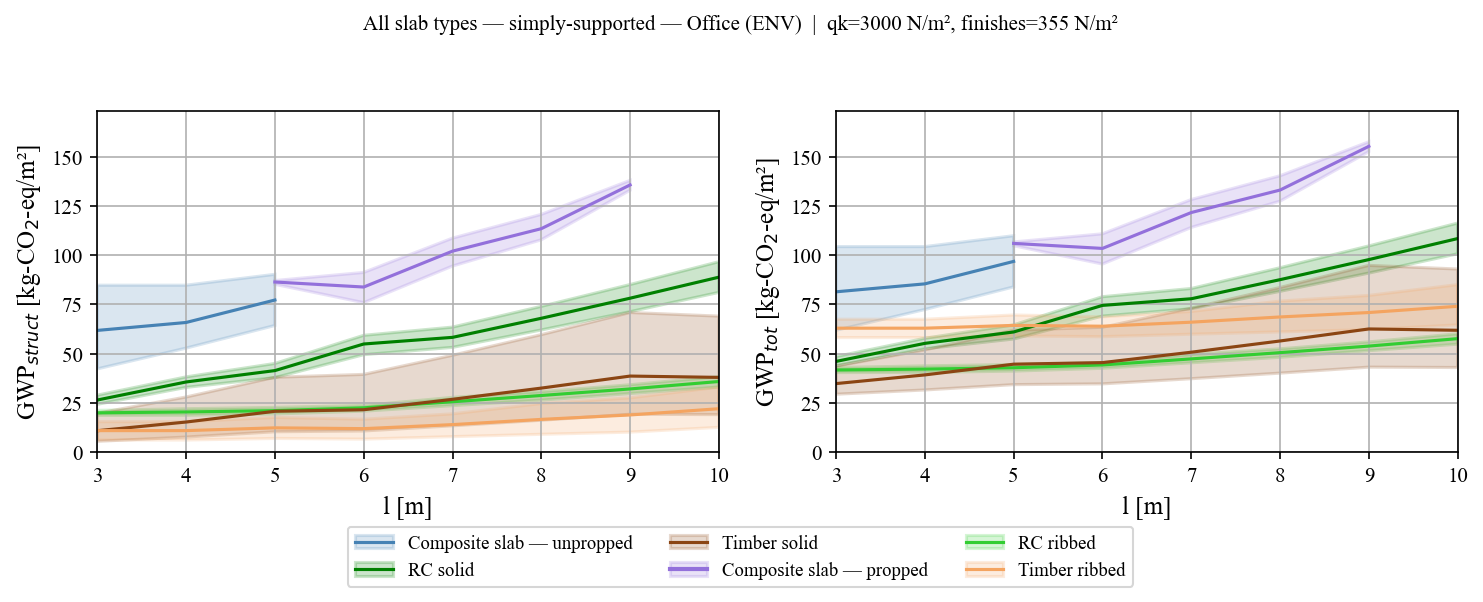
\includegraphics[width=\textwidth]{figures/office/ENV/plot_office_1span_ENV_gwp.png}
        \caption{Single span}
        \label{fig:office_gwp_1span}
    \end{subfigure}\\[4pt]
    \begin{subfigure}{\textwidth}
        \centering
        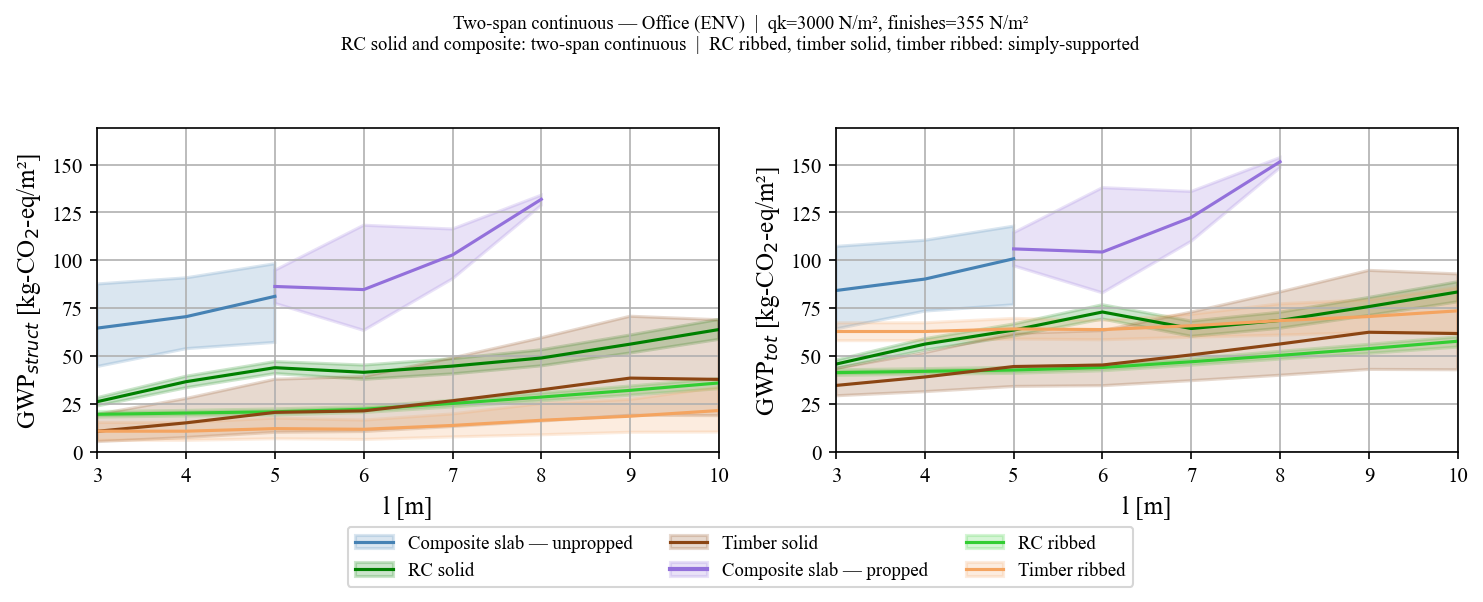
\includegraphics[width=\textwidth]{figures/office/ENV/plot_office_2span_ENV_gwp.png}
        \caption{Two--span continuous}
        \label{fig:office_gwp_2span}
    \end{subfigure}\\[4pt]
    \begin{subfigure}{\textwidth}
        \centering
        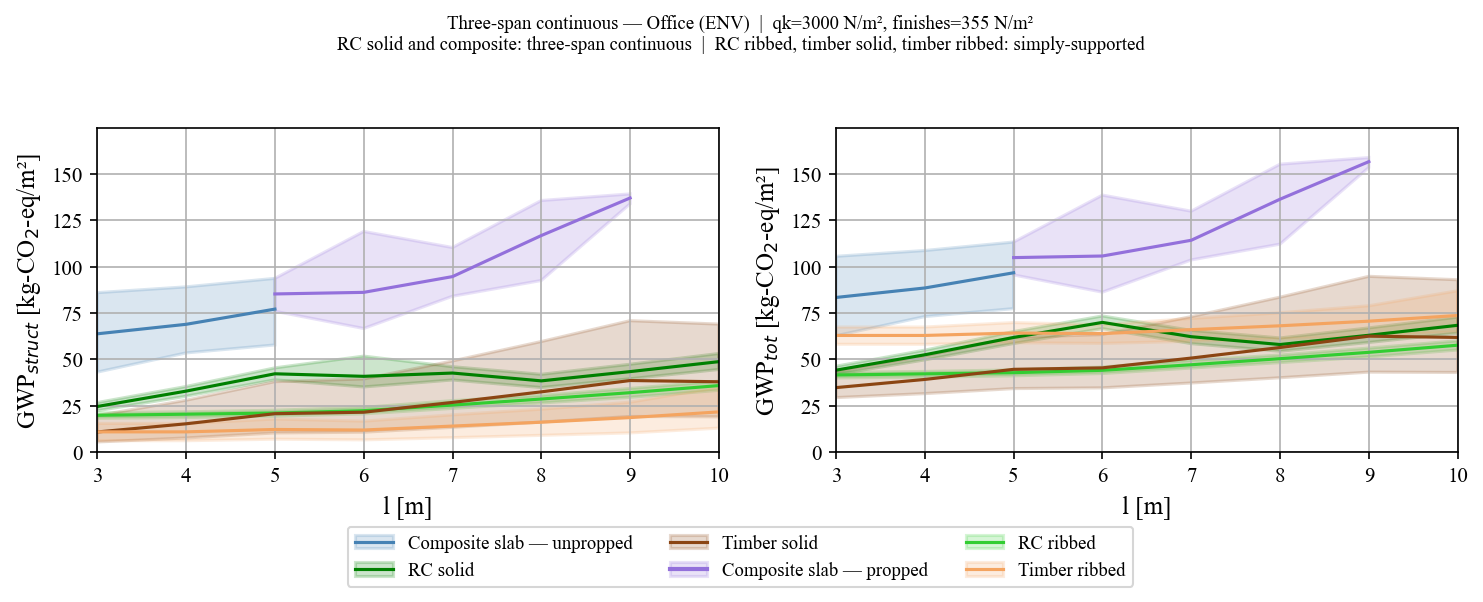
\includegraphics[width=\textwidth]{figures/office/ENV/plot_office_3span_ENV_gwp.png}
        \caption{Three--span continuous}
        \label{fig:office_gwp_3span}
    \end{subfigure}
    \caption[Office total GWP versus span]{Office scenario: total GWP per unit floor area versus span for all five floor systems, in the single--, two--, and three--span configurations.}
    \label{fig:office_gwp}
\end{figure}

The dominant result is unambiguous and holds across every span and span configuration: \textbf{the composite slab has the highest total GWP of the five systems compared}. For the single--span office case, the composite optimum rises from 67.6\,kg\,CO$_2$eq/m$^2$ at 3\,m to 152.5\,kg\,CO$_2$eq/m$^2$ at 9\,m, with no feasible solution at 10\,m. Over the same range the RC flat slab spans 43.8--100.7, the RC ribbed slab 40.3--54.8, the timber rectangular slab 29.3--43.1, and the timber ribbed slab 58.1--64.5\,kg\,CO$_2$eq/m$^2$. The timber rectangular slab is the lowest--carbon system throughout, and the RC ribbed slab the lowest of the non--timber systems. The timber ribbed slab, despite the label, carries comparable GWP to the RC flat slab: this reflects the higher GWP intensity of the engineered timber (glulam) used in the ribbed geometry relative to the solid timber used in the rectangular system, combined with the greater structural depth of the ribbed profile. At 3\,m the composite slab carries approximately 53\% more embodied carbon than the RC ribbed baseline; by 9\,m this gap widens to roughly a factor of three, as the composite GWP grows steeply with span while the RC ribbed and timber GWP grow only gradually.

Extending the composite and RC flat systems to continuous spans alters their GWP, but does not change the overall ranking: in no configuration does either system approach the RC ribbed or timber baselines. The effect of continuity on the composite slab is non--monotonic and is examined separately in Section~\ref{sec:res_office_continuity}.

\begin{table}[h!]
\small\centering
\caption{Optimal composite cross--sections, office scenario, all span configurations.}
\label{tab:office_optima}
\begin{tabular}{llcccccl}
\toprule
Config. & $L$ [m] & Deck & Grade & $h$ [mm] & $\mathrm{GWP}_\mathrm{tot}$ & Propped & Governing check \\
\midrule
\multirow{7}{*}{Single}
 & 3 & Multideck 80 1.0  & C25/30 & 198 & 67.6  & No  & Fire D1 \\
 & 4 & ComFlor 210       & C25/30 & 357 & 91.8  & No  & Fire D4 \\
 & 5 & Multideck 146 1.5 & C25/30 & 279 & 104.7 & No  & Fire D4 \\
 & 6 & ComFlor 210       & C25/30 & 365 & 95.4  & Yes & SLS deflection \\
 & 7 & ComFlor 225       & C25/30 & 441 & 114.0 & Yes & SLS deflection \\
 & 8 & ComFlor 225       & C25/30 & 504 & 127.4 & Yes & SLS deflection \\
 & 9 & Multideck 146 1.5 & C25/30 & 455 & 152.5 & Yes & SLS deflection \\
\midrule
\multirow{6}{*}{Two--span}
 & 3 & Multideck 80 1.0  & C25/30 & 198 & 65.9  & No  & Fire D1 \\
 & 4 & ComFlor 210       & C25/30 & 357 & 91.0  & No  & Fire D4 \\
 & 5 & ComFlor 225       & C25/30 & 363 & 97.1  & No  & Fire D3 \\
 & 6 & ComFlor 60 0.9    & C25/30 & 233 & 83.1  & Yes & ULS hogging \\
 & 7 & ComFlor 210       & C25/30 & 431 & 110.0 & Yes & Fire D3 \\
 & 8 & Multideck 146 1.5 & C25/30 & 470 & 148.4 & Yes & ULS hogging \\
\midrule
\multirow{7}{*}{Three--span}
 & 3 & Multideck 80 1.0  & C25/30 & 198 & 67.9  & No  & Fire D1 \\
 & 4 & ComFlor 210       & C25/30 & 357 & 91.0  & No  & Fire D4 \\
 & 5 & ComFlor 225       & C25/30 & 354 & 95.5  & No  & Fire D3 \\
 & 6 & ComFlor 60 0.9    & C30/37 & 240 & 86.2  & Yes & ULS hogging \\
 & 7 & ComFlor 210       & C25/30 & 398 & 103.6 & Yes & Fire D3 \\
 & 8 & ComFlor 210       & C25/30 & 439 & 112.1 & Yes & Fire D3 \\
 & 9 & Multideck 146 1.5 & C25/30 & 475 & 153.5 & Yes & ULS hogging \\
\bottomrule
\end{tabular}
\end{table}

%------------------------------------------------------------------
\subsubsection{Governing limit states}
\label{sec:res_office_gov}
%------------------------------------------------------------------
The limit state governing each composite optimum shifts systematically with span and configuration (Table~\ref{tab:office_optima}). For the \emph{single--span} optima, the fire thermal--insulation check (D1) governs at 3\,m, longitudinal shear by the m--k method at 4\,m, and composite SLS deflection at every span from 5\,m upward. For the \emph{continuous} configurations the hogging checks---composite ULS hogging and the fire D3 reduced--section hogging check---govern at most spans, reflecting the support moment that the single--span case does not carry.
 
That SLS deflection governs the single--span optima from 5\,m is confirmed by comparing the single--criterion runs. Figure~\ref{fig:office_criteria} overlays the GWP of the ULS--only, SLS--only, and fire--only optima against the combined envelope (ENV) result, for each span configuration. For the single span (Figure~\ref{fig:office_criteria}a), the envelope follows the SLS--only curve closely from 5\,m upward, with the ULS--only curve sitting consistently below and the fire--only remaining relatively constant ---confirming that the single--span slab is stiffness--governed at practical spans rather than strength--governed. This is a key observation, since the added depth and hence GWP is being driven by deflection control rather than by load capacity.
 
For the continuous configurations (Figures~\ref{fig:office_criteria}b and~\ref{fig:office_criteria}c) the picture changes: the envelope departs from the SLS--only curve and rises above both the SLS-- and ULS--only curves at several spans, the ULS--curve in this case is higher than the SLS, showing that at continuous spans the strength governs the design. In all configurations the fire--only curve is the lowest and flattest, confirming that fire governs only at the shortest spans.

\begin{figure}[h!]
    \centering
    \begin{subfigure}{\textwidth}
        \centering
        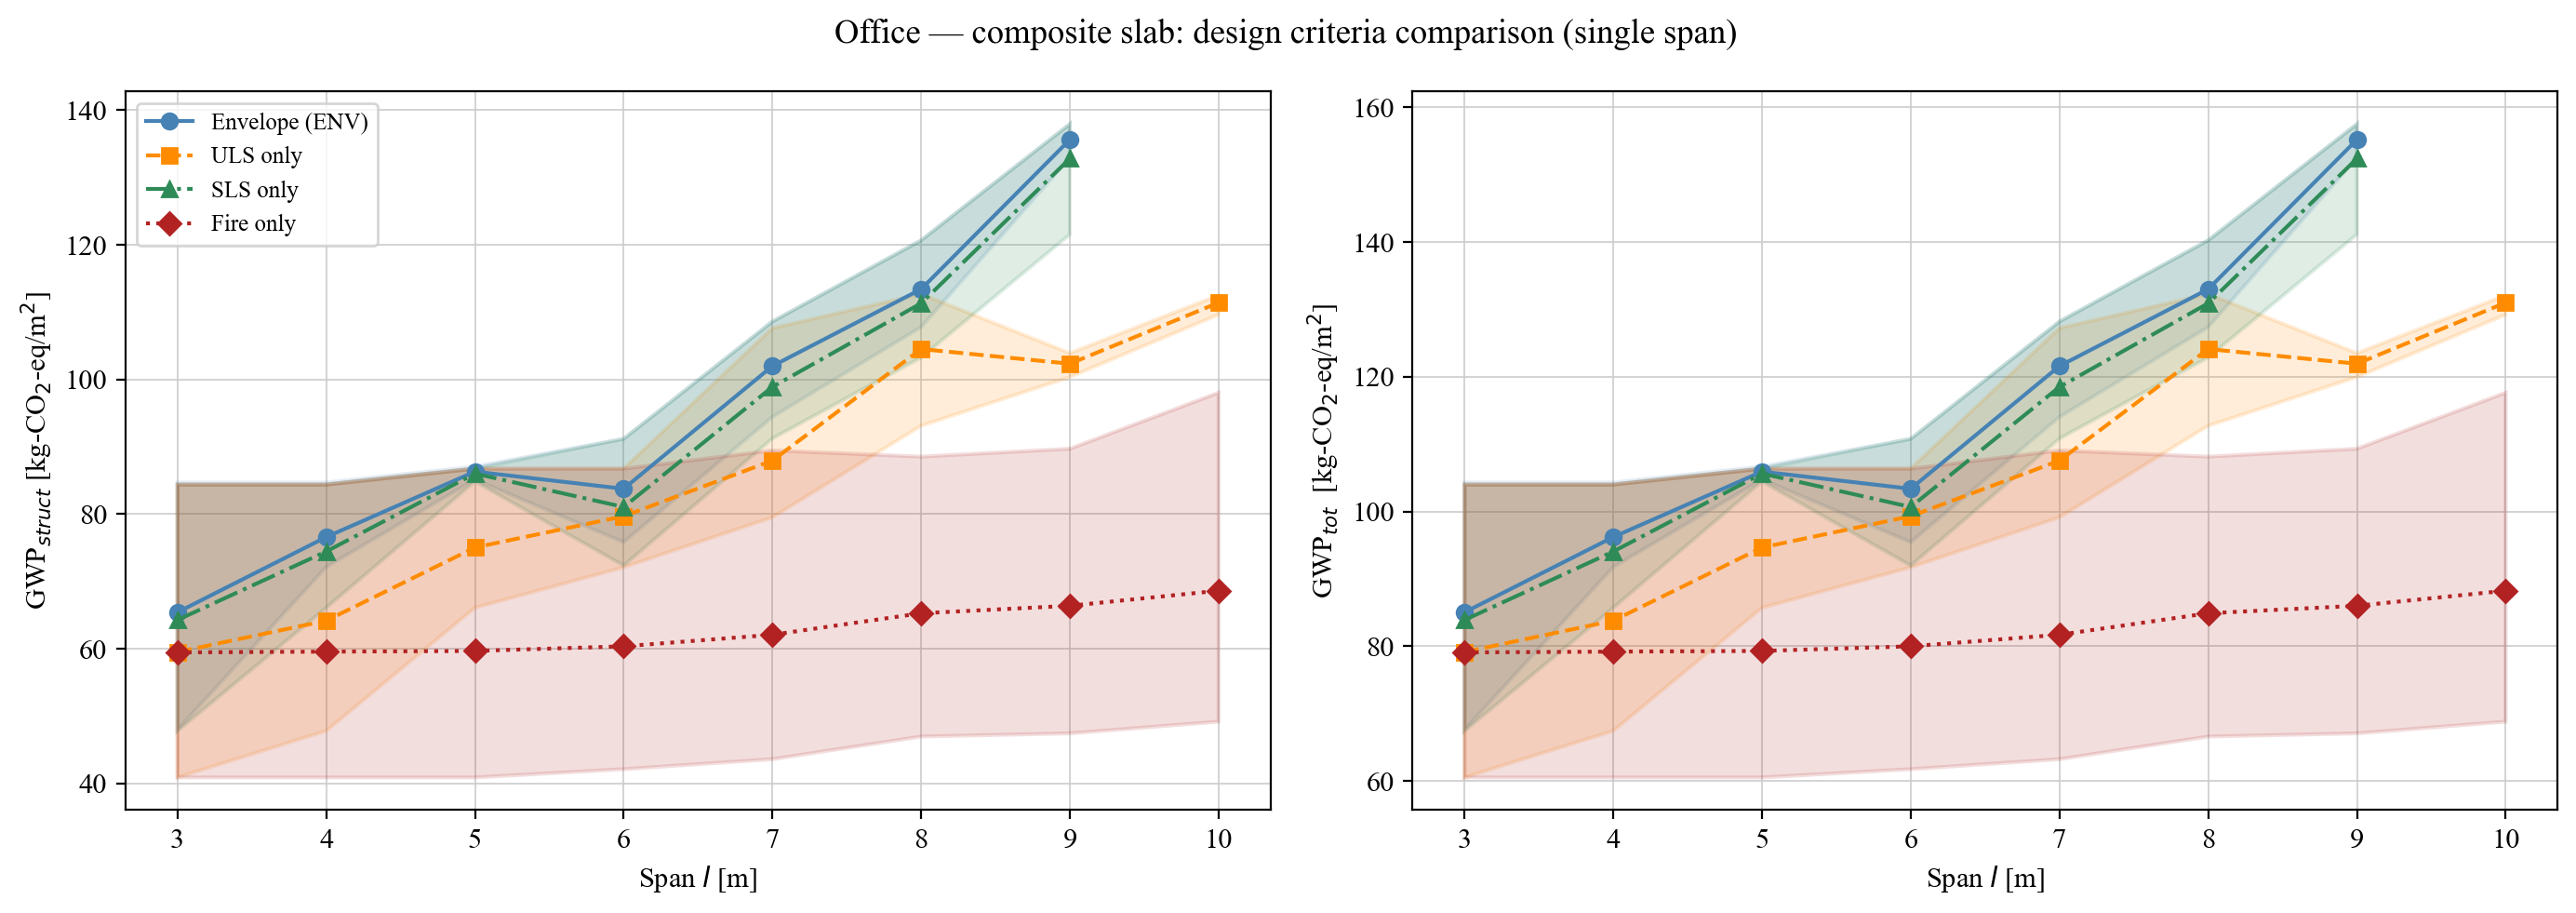
\includegraphics[width=\textwidth]{figures/office/fig_criteria_comparison_SS.png}
        \caption{Single span}
        \label{fig:office_criteria_SS}
    \end{subfigure}\\[4pt]
    \begin{subfigure}{\textwidth}
        \centering
        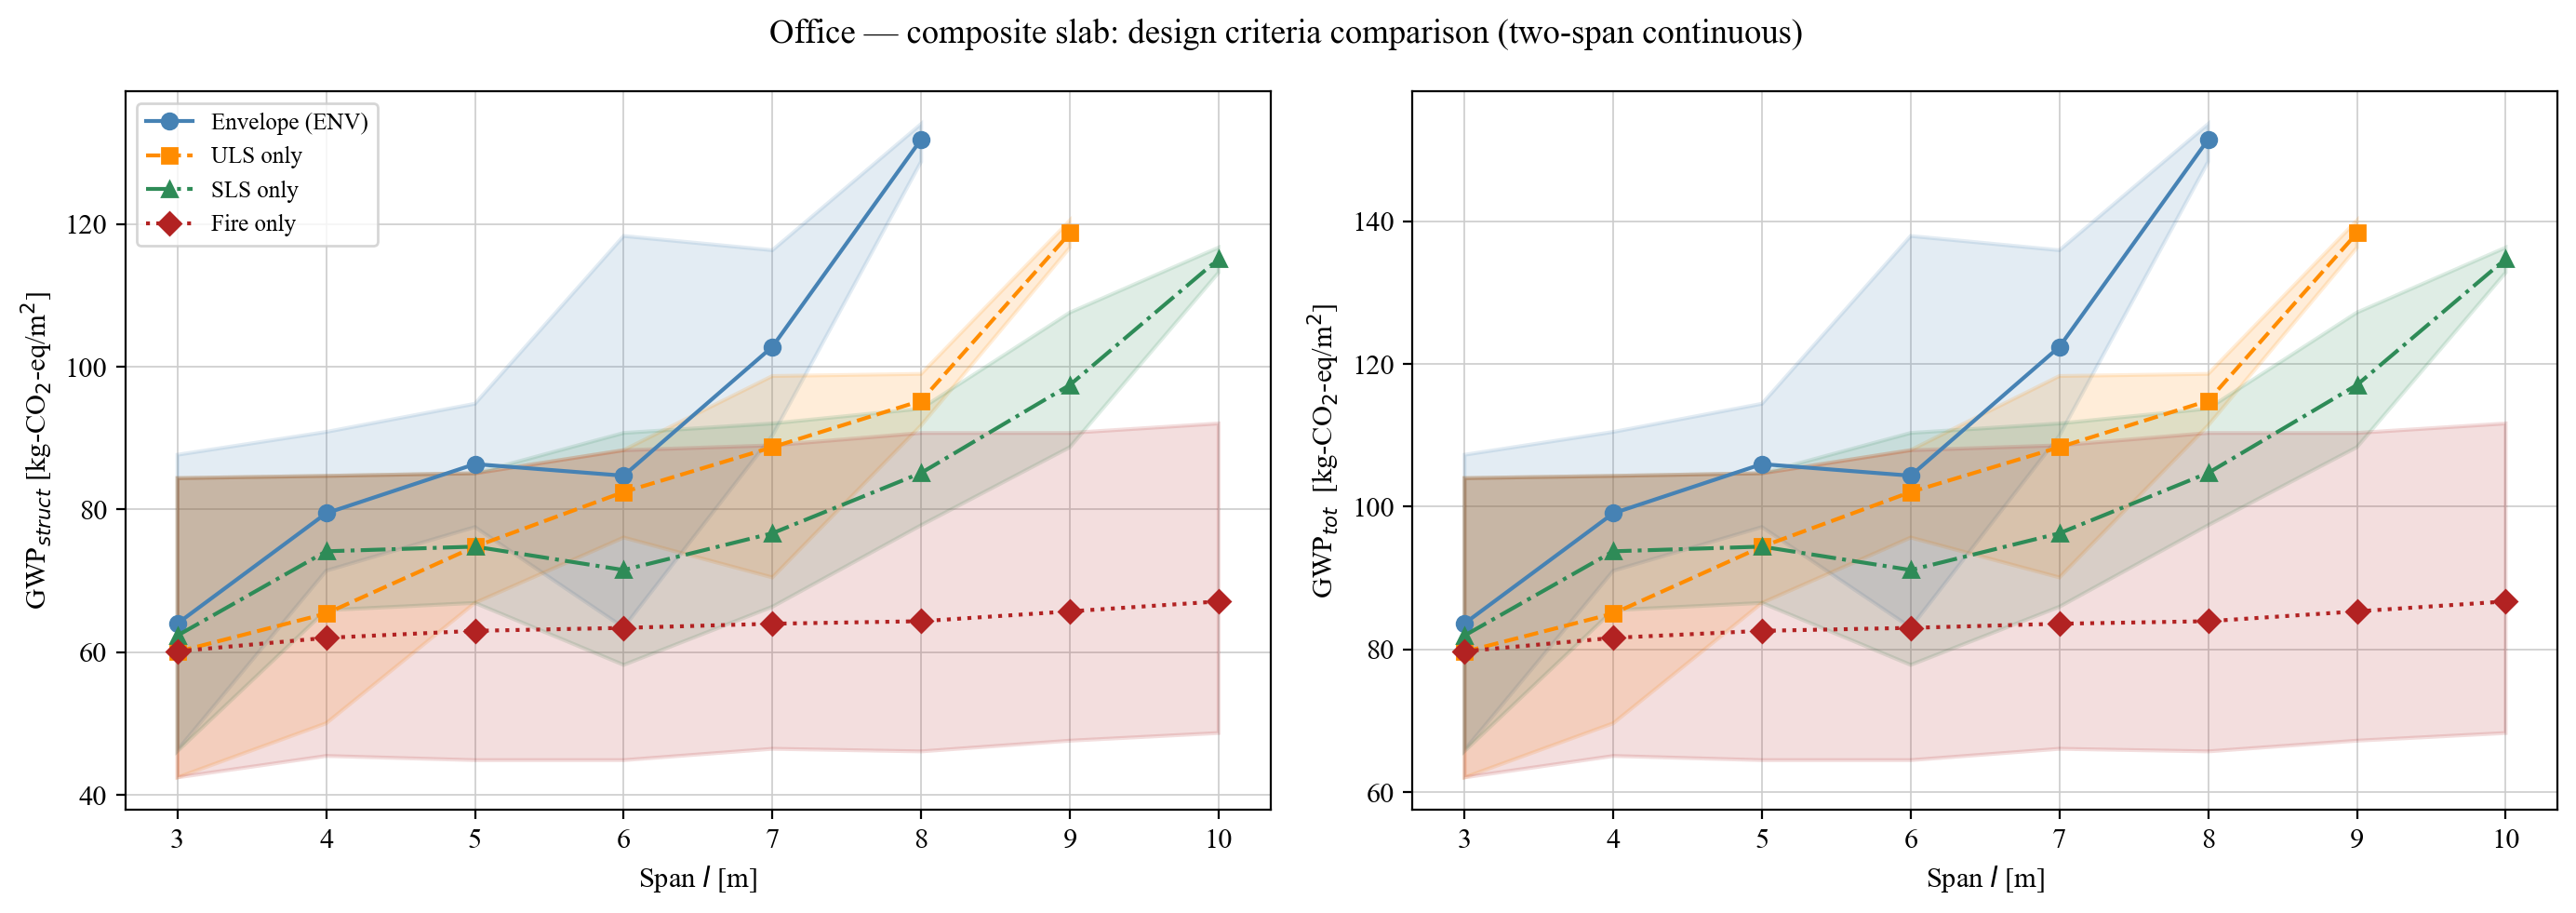
\includegraphics[width=\textwidth]{figures/office/fig_criteria_comparison_2span.png}
        \caption{Two--span continuous}
        \label{fig:office_criteria_2span}
    \end{subfigure}\\[4pt]
    \begin{subfigure}{\textwidth}
        \centering
        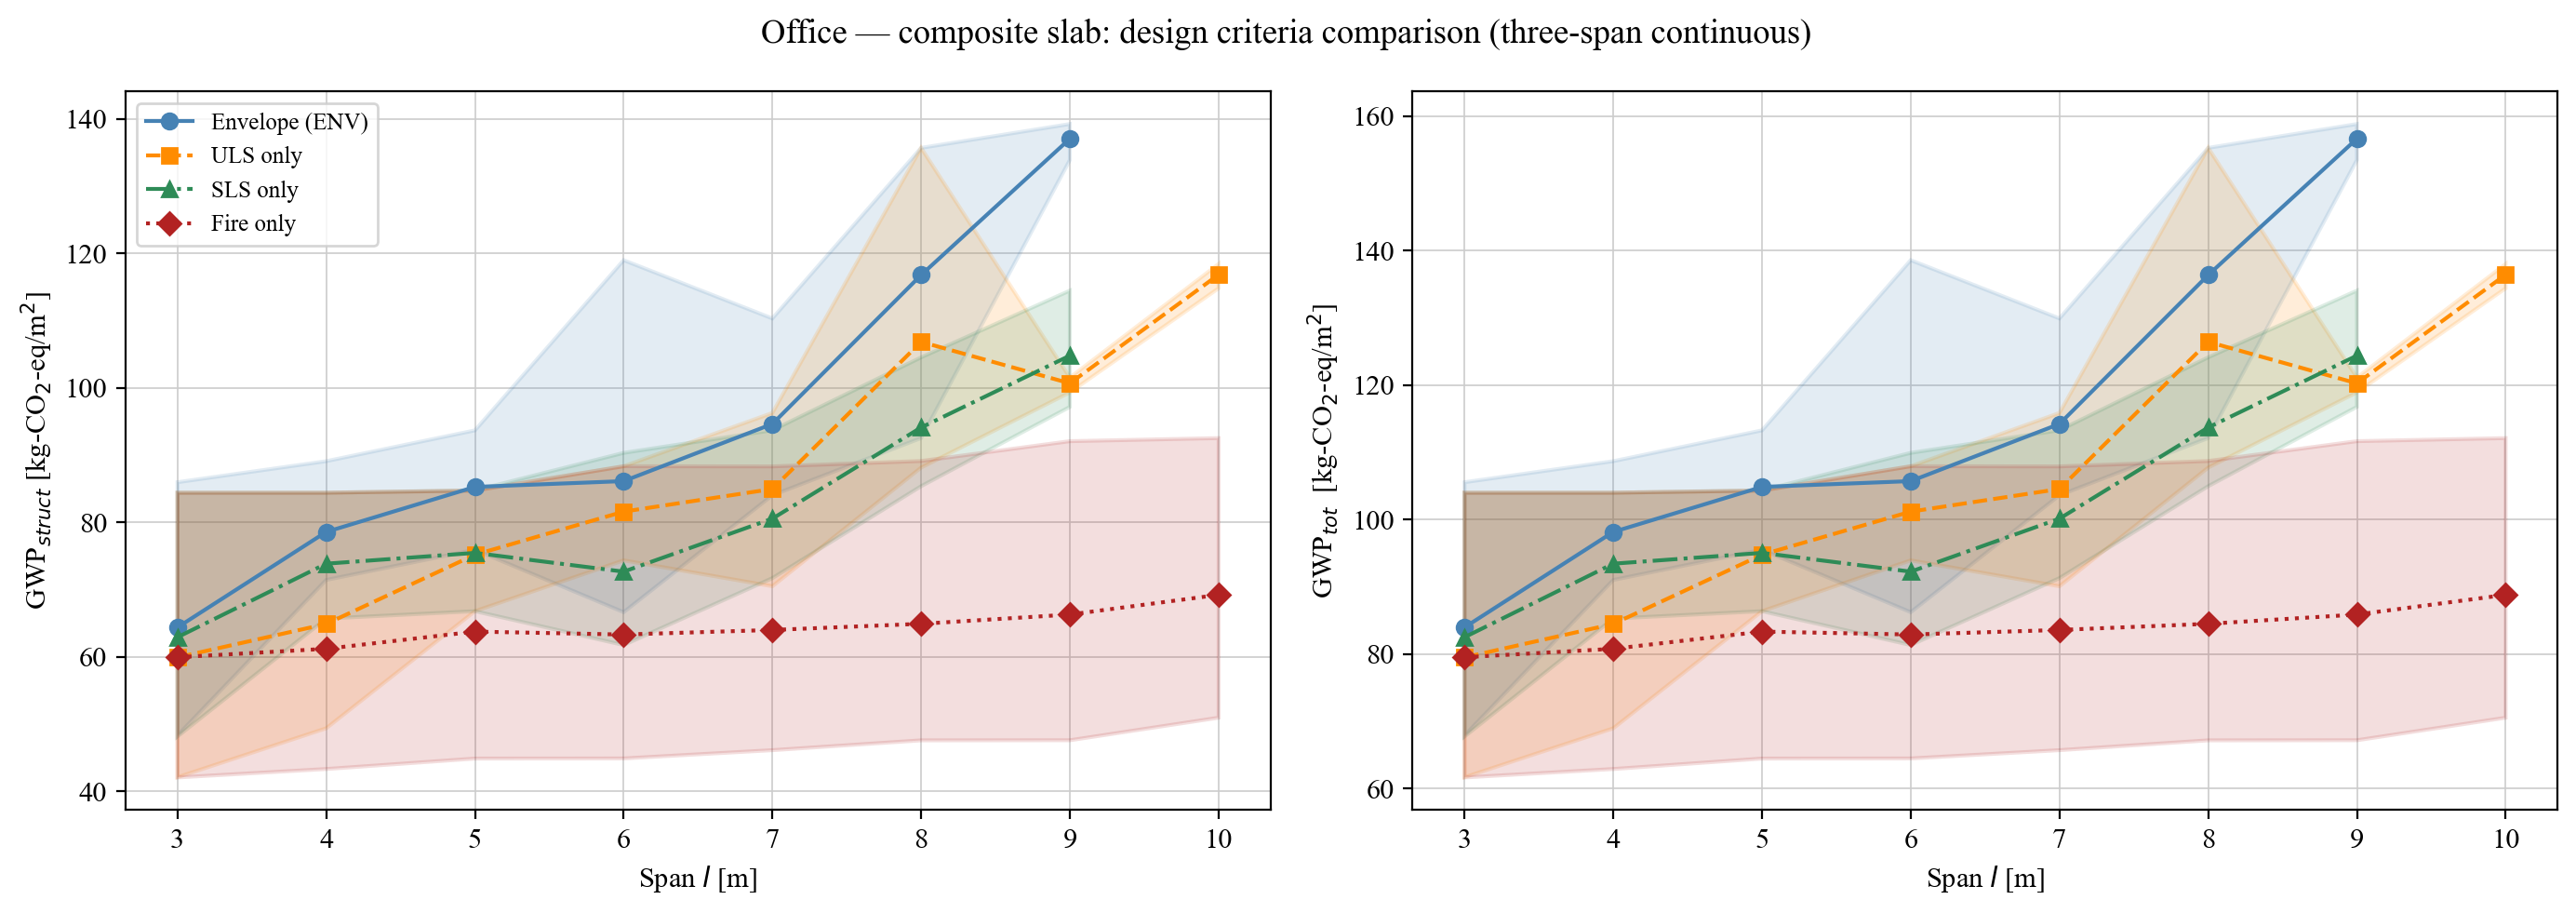
\includegraphics[width=\textwidth]{figures/office/fig_criteria_comparison_3span.png}
        \caption{Three--span continuous}
        \label{fig:office_criteria_3span}
    \end{subfigure}
    \caption[Office composite design criteria comparison]{Office composite slab: GWP of the optima obtained under each design criterion in isolation (ULS only, SLS only, fire only) compared with the combined envelope (ENV), for the single--, two--, and three--span configurations.}
    \label{fig:office_criteria}
\end{figure}

Examining the feasible solution space shows that unpropped construction is feasible only up to 5\,m in every span configuration. At 3\,m, 32 deck--grade combinations satisfy all checks unpropped (single span); this falls to 16 at 4\,m and just 4 at 5\,m, and from 6\,m upward no deck in the database can carry the wet--concrete construction load unpropped within the 300\,mm depth bound. The two-- and three--span configurations show the same cliff at 6\,m, with marginally more unpropped options surviving at 5\,m (8 each) because continuity of the bare deck over the supports slightly reduces the construction--stage sagging moment. Since the construction stage is carried by the steel deck alone---before composite action develops---the number of final spans has little influence on where unpropped construction runs out.

Critically, propping lowers GWP even at spans where unpropped construction remains feasible. At 3\,m the lightest feasible unpropped single--span section carries 67.6\,kg\,CO$_2$eq/m$^2$ against 61.8 propped; at 5\,m the gap widens to 104.7 versus 83.8\,kg\,CO$_2$eq/m$^2$. Unpropped construction forces a heavier, deeper deck purely to survive the wet--concrete pour, whereas propping removes that constraint and allows the section to be sized by the in--service limit states. Propping therefore would be selected throughout the office range below 6\,m because it yields the lower--carbon section, if the unpropped preference encoded in the optimisation routine were not applied.

The upper feasibility limit differs by configuration. The single-- and three--span cases remain feasible (propped) up to 9\,m, but the \textbf{two--span configuration becomes infeasible beyond 8\,m}---one span sooner---because the hogging moment at the single internal support is the most severe of the three arrangements, and no deck--reinforcement combination can satisfy the hogging ULS and fire D3 checks at 9\,m within the depth bound. The three--span case distributes the support moments more favourably and recovers feasibility at 9\,m. No configuration is feasible at 10\,m: at that span the composite SLS deflection check cannot be satisfied within the 500\,mm depth bound for any deck in the database, even with propped construction.

%------------------------------------------------------------------
\subsubsection{GWP breakdown by material}
\label{sec:res_office_breakdown}
%------------------------------------------------------------------
Table~\ref{tab:office_breakdown} decomposes the single--span composite GWP into its material contributions. The steel deck is the single largest structural contributor at most spans, exceeding the concrete contribution up to 6\,m and remaining comparable beyond it, despite the steel mass being far smaller than the concrete mass---a direct consequence of the much higher GWP intensity per kilogram of structural steel. The fixed floor build--up (19.6\,kg\,CO$_2$eq/m$^2$) is 32\% of the total at 3\,m but only 13\% at 9\,m, as the structural contribution grows with span.

\begin{table}[h!]
\small\centering
\caption{GWP breakdown of the optimal composite slab, office single span (kg\,CO$_2$eq/m$^2$).}
\label{tab:office_breakdown}
\begin{tabular}{ccccccc}
\toprule
$L$ [m] & Concrete & Deck & Mesh & Trough bars & Struct. & Build--up \\
\midrule
3 & 15.1 & 23.4 & 1.6 & 2.2  & 42.2  & 19.6 \\
4 & 19.2 & 28.8 & 2.4 & 2.4  & 52.7  & 19.6 \\
5 & 28.9 & 29.2 & 2.4 & 3.7  & 64.2  & 19.6 \\
6 & 24.8 & 46.9 & 2.4 & 1.7  & 75.8  & 19.6 \\
7 & 41.2 & 49.1 & 2.4 & 1.7  & 94.4  & 19.6 \\
8 & 53.2 & 49.1 & 2.4 & 3.1  & 107.8 & 19.6 \\
9 & 54.9 & 60.8 & 2.4 & 14.8 & 132.9 & 19.6 \\
\bottomrule
\end{tabular}
\end{table}

The fire trough--bar contribution is small at most spans but jumps to 14.8\,kg\,CO$_2$eq/m$^2$ at 9\,m, where the deep section requires substantial trough reinforcement to satisfy the D2 fire sagging check. Figure~\ref{fig:office_breakdown} shows the breakdown as a stacked bar for the single span; the equivalent figures for the two-- and three--span configurations are given in Appendix~\ref{app:results_figures}.

\begin{figure}[h!]
    \centering
    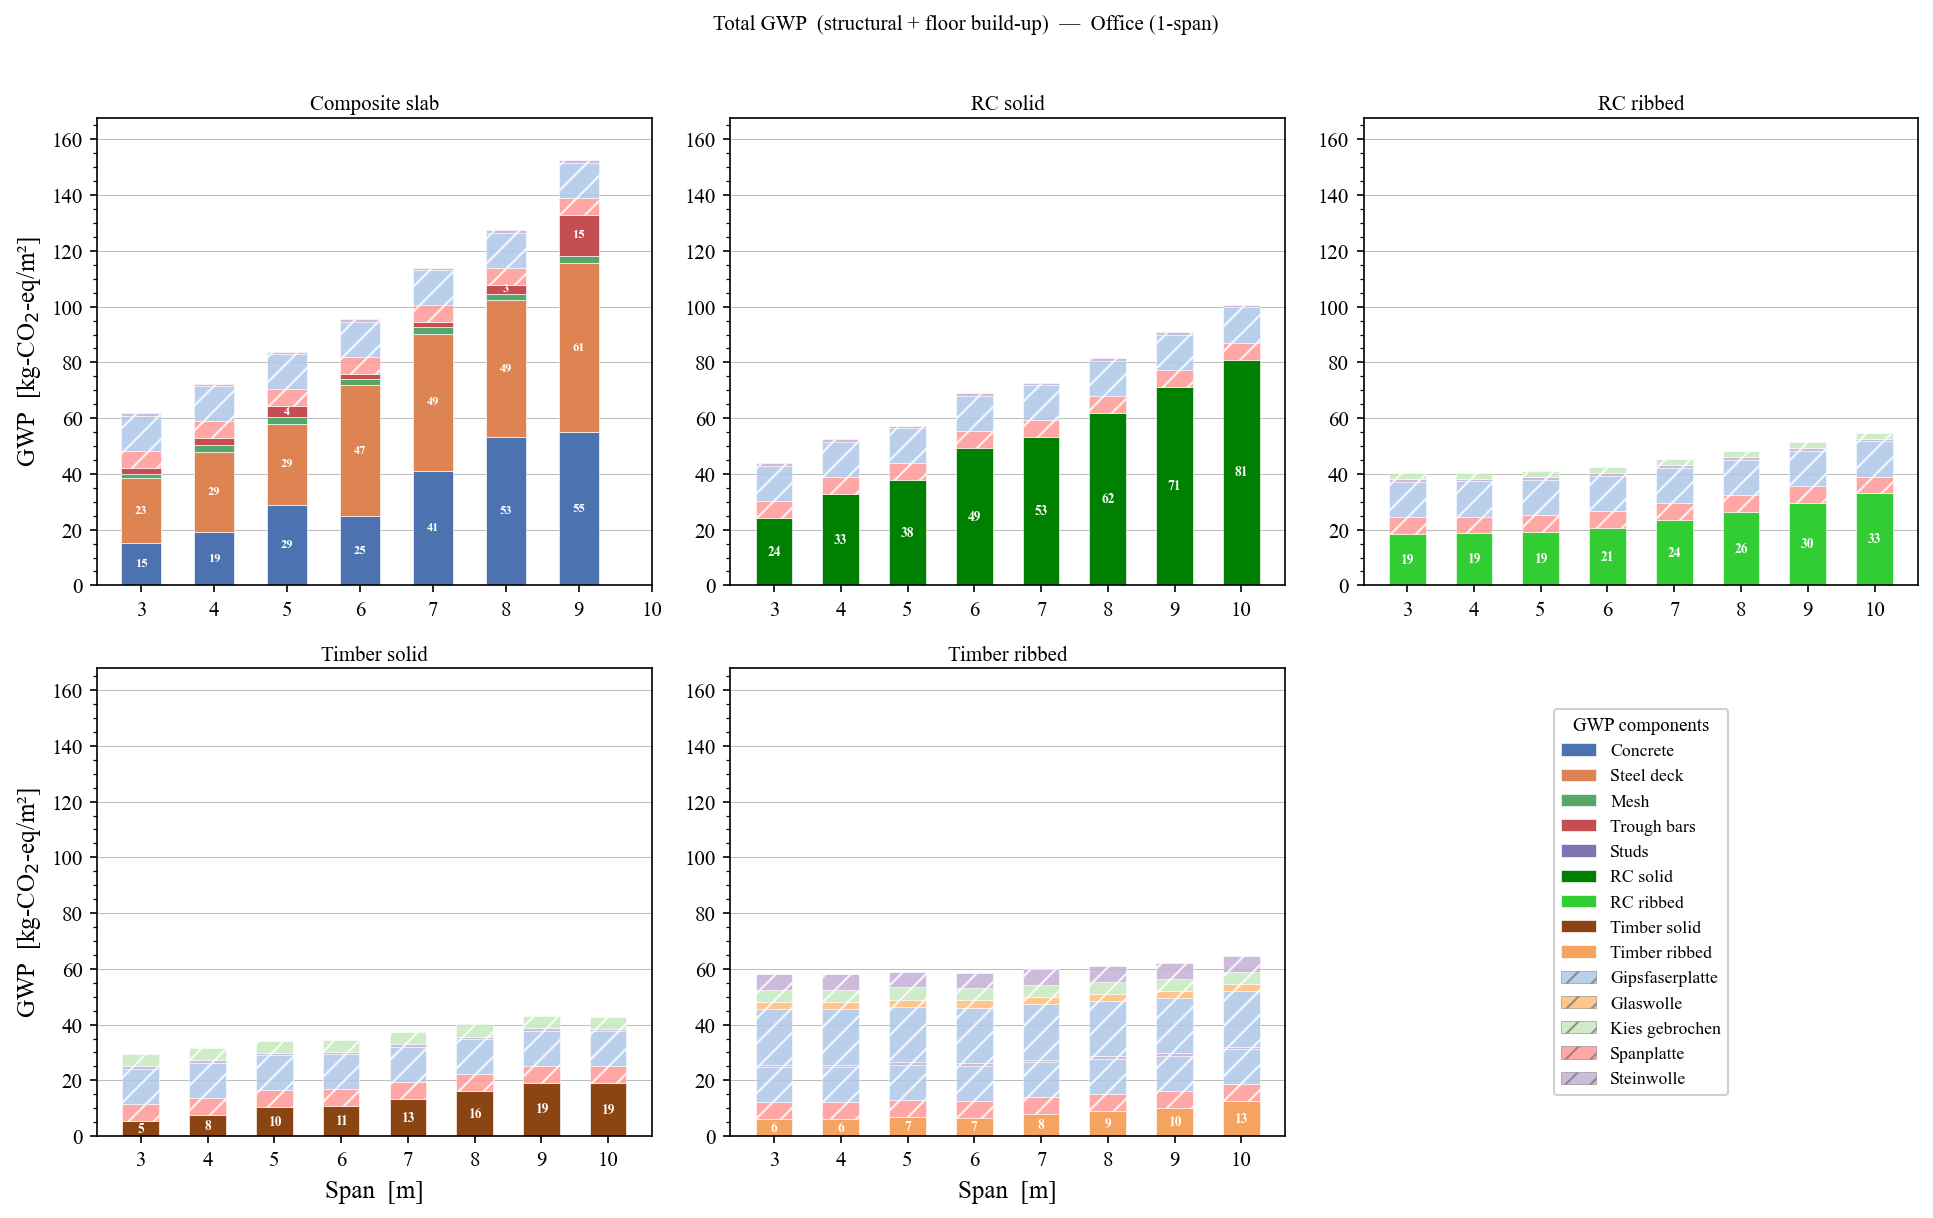
\includegraphics[width=\textwidth]{figures/office/GWP breakdown/results_office_ENV_gwp_total.png}
    \caption[Office GWP breakdown, single span]{Office single span: total GWP of the optimal slab.}
    \label{fig:office_breakdown}
\end{figure}

%------------------------------------------------------------------
\subsubsection{Structural depth and mass}
\label{sec:res_office_depth}
%------------------------------------------------------------------
Figure~\ref{fig:office_height} compares the structural depth ($h_\mathrm{struct}$) and total depth ($h_\mathrm{tot}$, including the floor build--up) of the five systems against span, for all three span configurations. The composite curve distinguishes the unpropped optimum (feasible only to 5\,m) from the propped optimum, which is the governing optimum across the full range (Section~\ref{sec:res_office_gov}).

\begin{figure}[h!]
    \centering
    \begin{subfigure}{\textwidth}
        \centering
        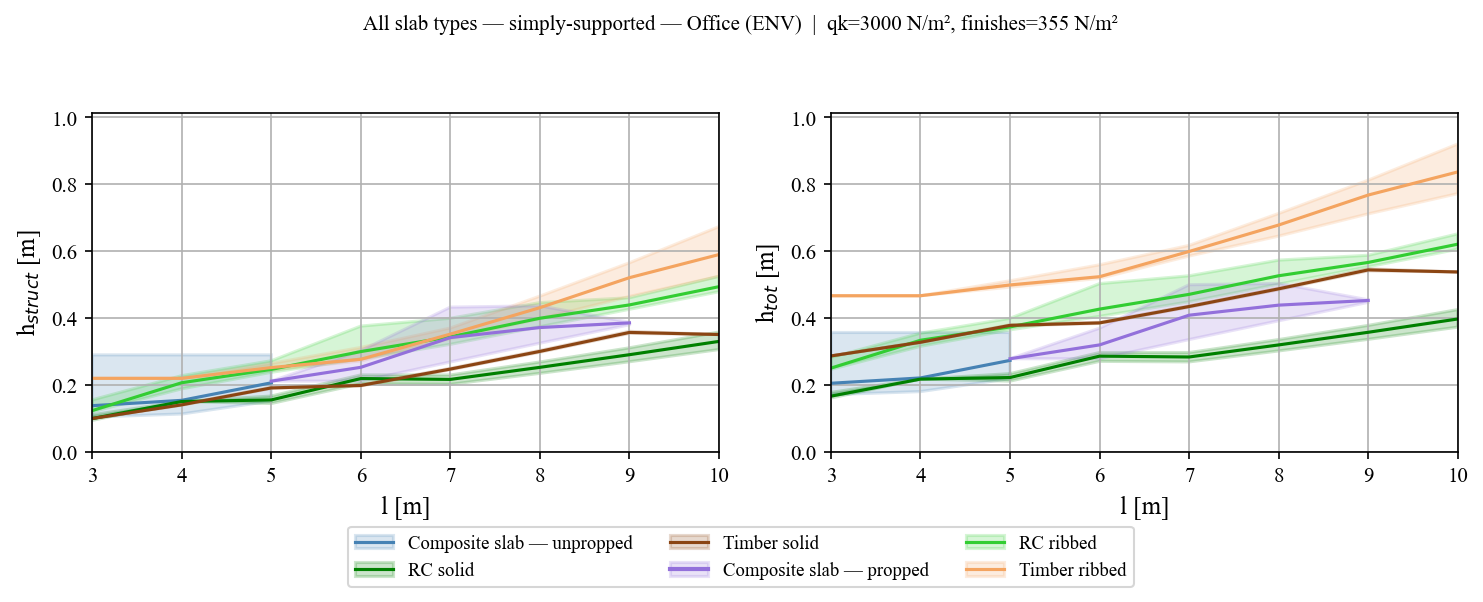
\includegraphics[width=\textwidth]{figures/office/ENV/plot_office_1span_ENV_height.png}
        \caption{Single span}
        \label{fig:office_height_SS}
    \end{subfigure}\\[4pt]
    \begin{subfigure}{\textwidth}
        \centering
        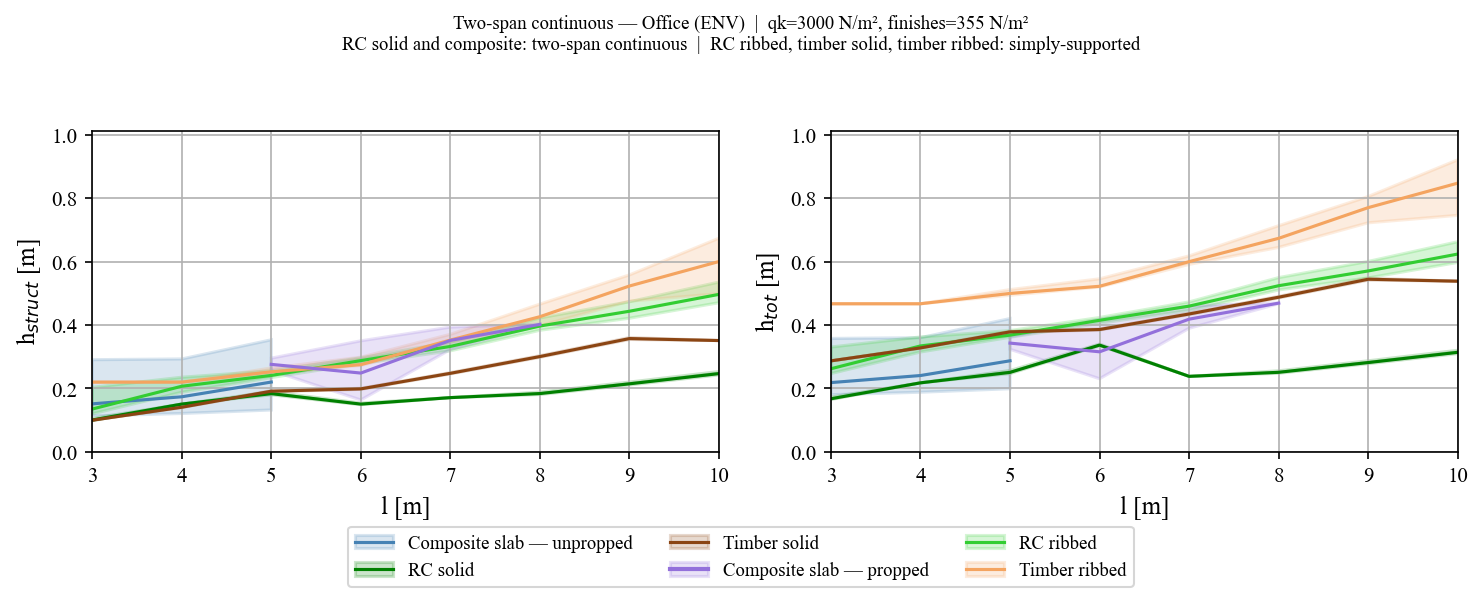
\includegraphics[width=\textwidth]{figures/office/ENV/plot_office_2span_ENV_height.png}
        \caption{Two--span continuous}
        \label{fig:office_height_2span}
    \end{subfigure}\\[4pt]
    \begin{subfigure}{\textwidth}
        \centering
        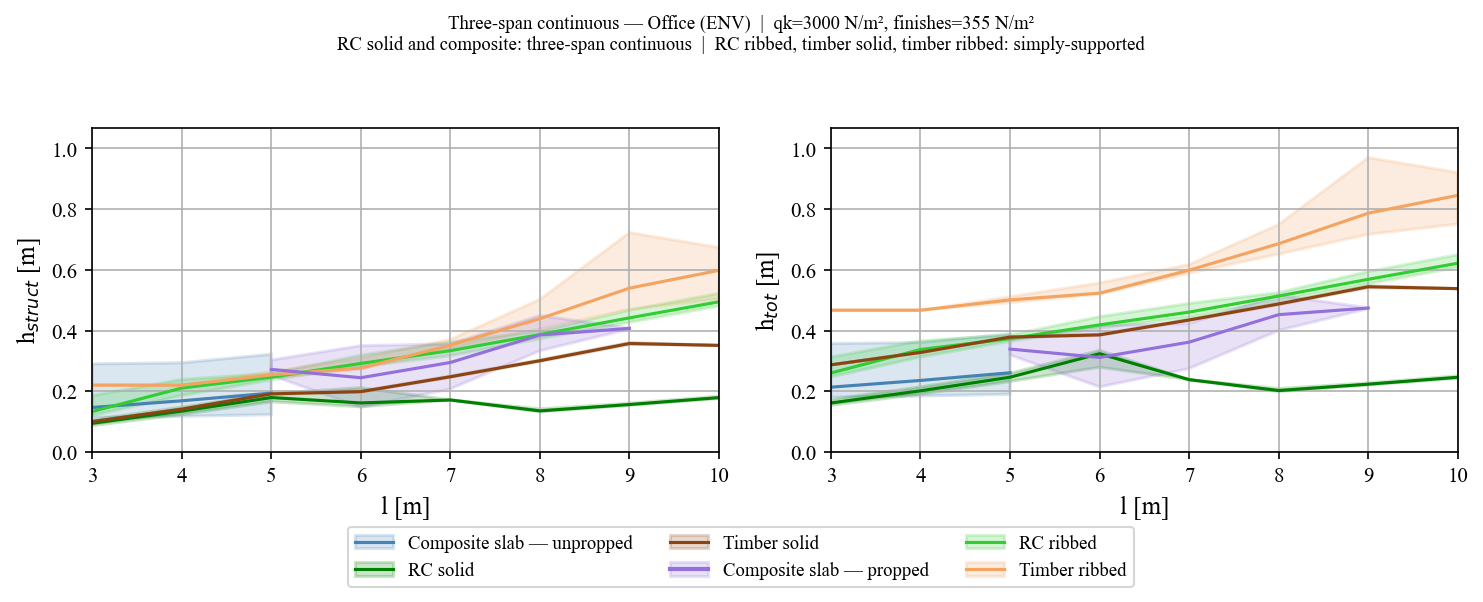
\includegraphics[width=\textwidth]{figures/office/ENV/plot_office_3span_ENV_height.png}
        \caption{Three--span continuous}
        \label{fig:office_height_3span}
    \end{subfigure}
    \caption[Office slab depth versus span]{Office scenario: structural depth $h_\mathrm{struct}$ (left) and total depth $h_\mathrm{tot}$ (right) versus span for all five systems, in the single--, two--, and three--span configurations.}
    \label{fig:office_height}
\end{figure}

The optimal composite depth grows with span in two distinct regimes. At short spans the section is shallow and nearly constant across configurations---the single--, two--, and three--span optima are all 180--185\,mm total at 3\,m---because the depth here is set by the fire thermal--insulation minimum rather than by strength or stiffness. As span increases, the optimiser selects a shallow trapezoidal deck (ComFlor~60, Multideck~80) until the deflection limit (single span) or the support hogging check (continuous spans) can no longer be met, at which point it steps abruptly to a deep deck (ComFlor~210/225). This produces a characteristic jump in depth: for the single span the total depth rises from 249\,mm at 5\,m to 365\,mm at 6\,m, whereas the continuous configurations select a shallow section for one span further---233--240\,mm at 6\,m---before jumping to roughly 400--430\,mm at 7\,m. Continuity therefore defers the transition to deep decking by approximately one span, because the reduced sagging moment over continuous supports keeps the shallow deck viable for longer.

Relative to the other systems, the composite slab is competitive on total depth despite its high embodied carbon. At the longest feasible spans its total depth (around 455\,mm at 9\,m, single span) is the second--shallowest of the five systems, exceeded only by the RC flat slab and sitting well below the RC ribbed and both timber systems. This shallow structural depth is one of the practical advantages of composite construction that the carbon comparison alone does not capture, and is returned to in the discussion (Chapter~\ref{fifthchapter}).

Grade C25/30 is selected in every optimum except the 6\,m three--span case, confirming that the section is not concrete--strength--governed; a stronger grade offers negligible structural benefit at higher GWP intensity.

The structural mass of the optimal sections is shown in Figure~\ref{fig:office_mass}. Broadly the mass tracks GWP, as expected since embodied carbon scales with material quantity, but the correspondence is not exact and the divergences are informative.
 
\begin{figure}[h!]
    \centering
    \begin{subfigure}{\textwidth}
        \centering
        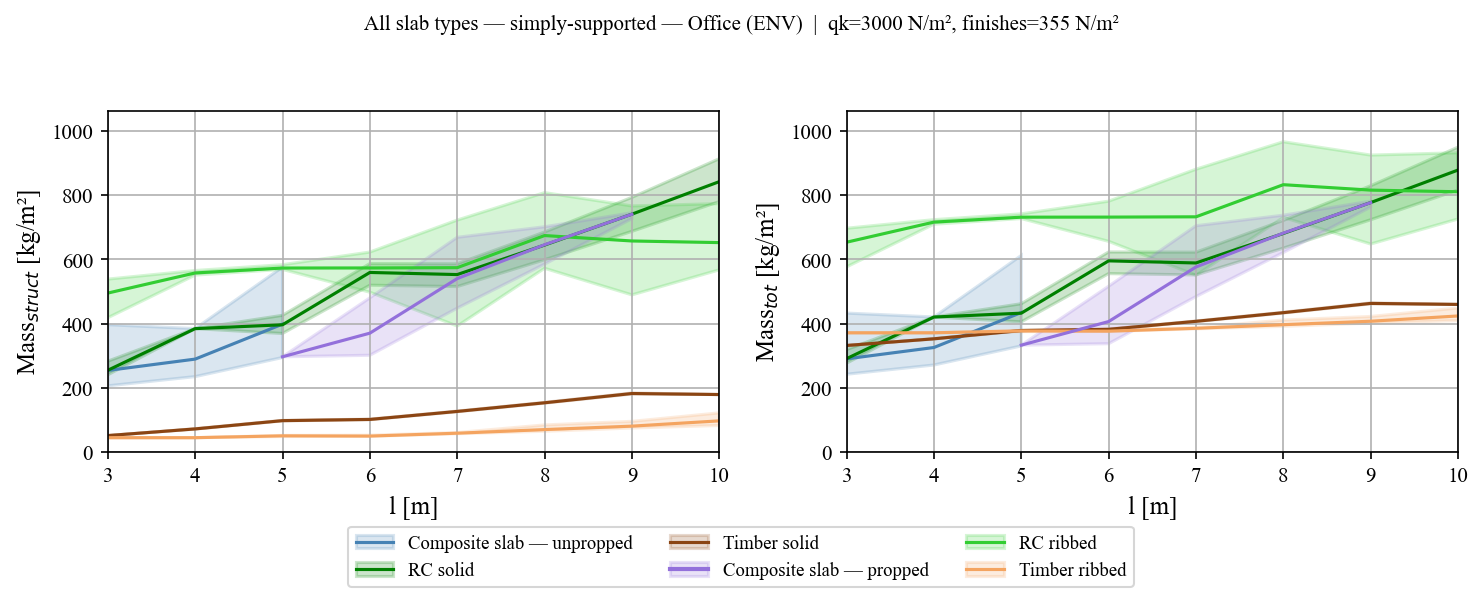
\includegraphics[width=\textwidth]{figures/office/ENV/plot_office_1span_ENV_mass.png}
        \caption{Single span}
        \label{fig:office_mass_SS}
    \end{subfigure}\\[4pt]
    \begin{subfigure}{\textwidth}
        \centering
        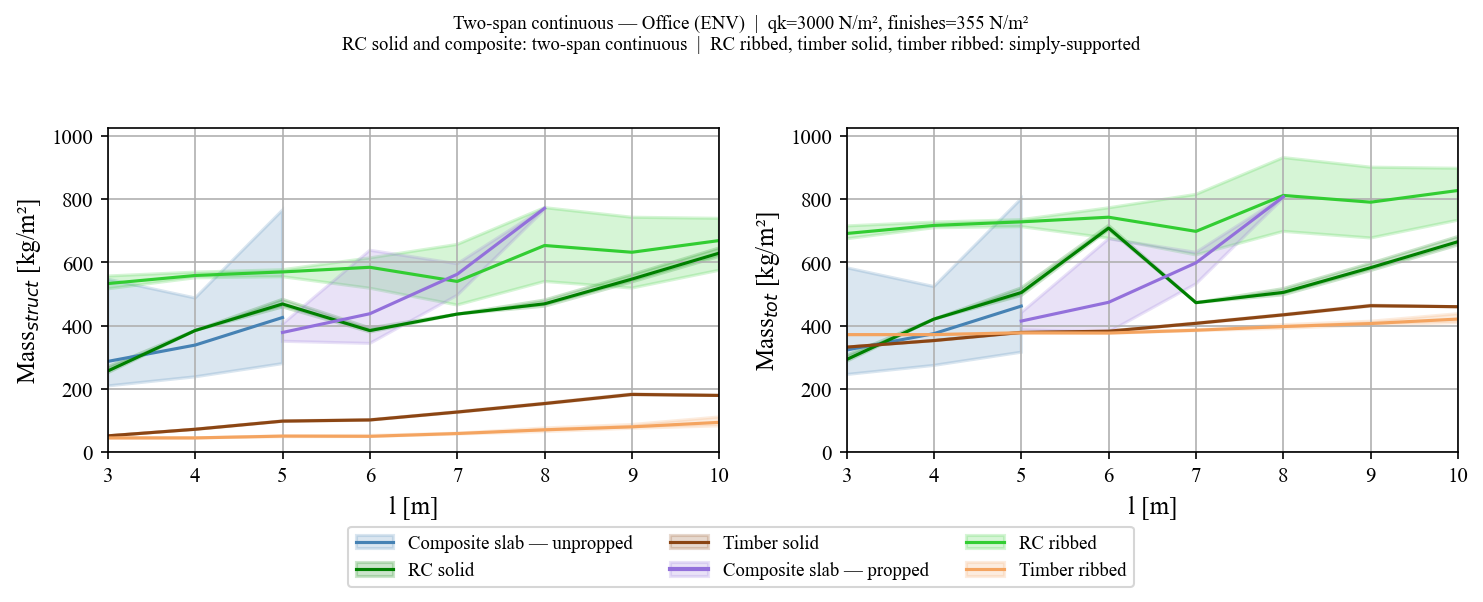
\includegraphics[width=\textwidth]{figures/office/ENV/plot_office_2span_ENV_mass.png}
        \caption{Two--span continuous}
        \label{fig:office_mass_2span}
    \end{subfigure}\\[4pt]
    \begin{subfigure}{\textwidth}
        \centering
        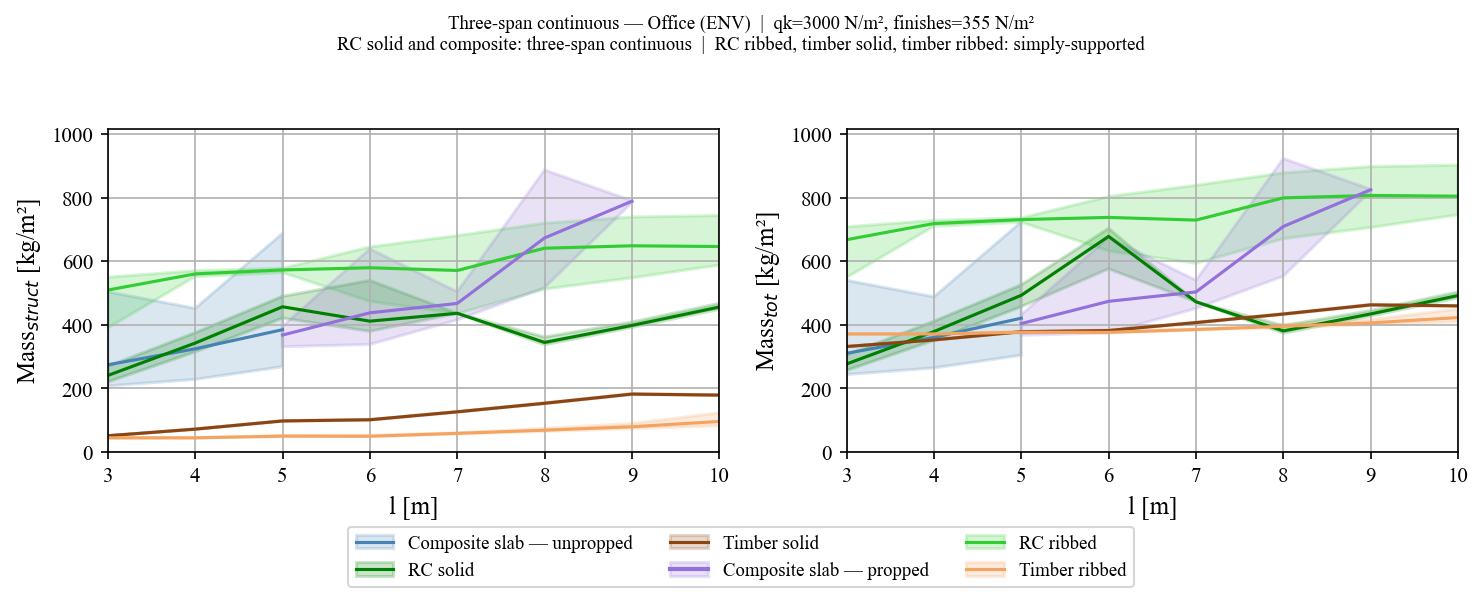
\includegraphics[width=\textwidth]{figures/office/ENV/plot_office_3span_ENV_mass.png}
        \caption{Three--span continuous}
        \label{fig:office_mass_3span}
    \end{subfigure}
    \caption[Office slab mass versus span]{Office scenario: structural mass $\mathrm{Mass}_\mathrm{struct}$ (left) and total mass $\mathrm{Mass}_\mathrm{tot}$ (right) per unit floor area versus span for all five systems, in the single--, two--, and three--span configurations.}
    \label{fig:office_mass}
\end{figure}
 
The composite slab is a heavy floor system, comparable in mass to reinforced concrete and far heavier than timber. The single--span composite optimum rises from 242\,kg/m$^2$ at 3\,m to 781\,kg/m$^2$ at 9\,m, almost entirely concrete; over the same range the two timber systems remain between roughly 370 and 460\,kg/m$^2$, so the composite slab is approximately twice the mass of an equivalent timber floor at the longer spans. This is a direct consequence of the cast in--situ concrete, which dominates the cross--section by mass even though the steel deck dominates by embodied carbon.
 
The most important observation is that mass and GWP do not rank the systems identically. The composite slab carries \textit{less} structural mass than the RC flat slab at the longer spans---745\,kg/m$^2$ against roughly 840\,kg/m$^2$ at 9\,m---yet has a substantially higher GWP. The composite slab's carbon penalty therefore arises from the high embodied--carbon intensity of the profiled steel deck per kilogram, not from the quantity of material in the floor. This reinforces the GWP breakdown of Section~\ref{sec:res_office_breakdown}, in which the steel deck is the largest single contributor to structural GWP despite being a small fraction of the mass.
 
This mass has consequences beyond embodied carbon---for foundation and column loads, and for the seismic mass of the structure---that are considered in the discussion (Chapter~\ref{fifthchapter}).

%------------------------------------------------------------------
\subsubsection{Effect of span continuity}
\label{sec:res_office_continuity}
%------------------------------------------------------------------
Figure~\ref{fig:office_continuity} plots the composite GWP optimum for the single--, two--, and three--span configurations on a single axis. The effect of continuity on the composite slab is small and non--monotonic, and it contrasts sharply with the reinforced concrete flat slab, for which continuity reduces GWP increasingly with span.

\begin{figure}[h!]
    \centering
    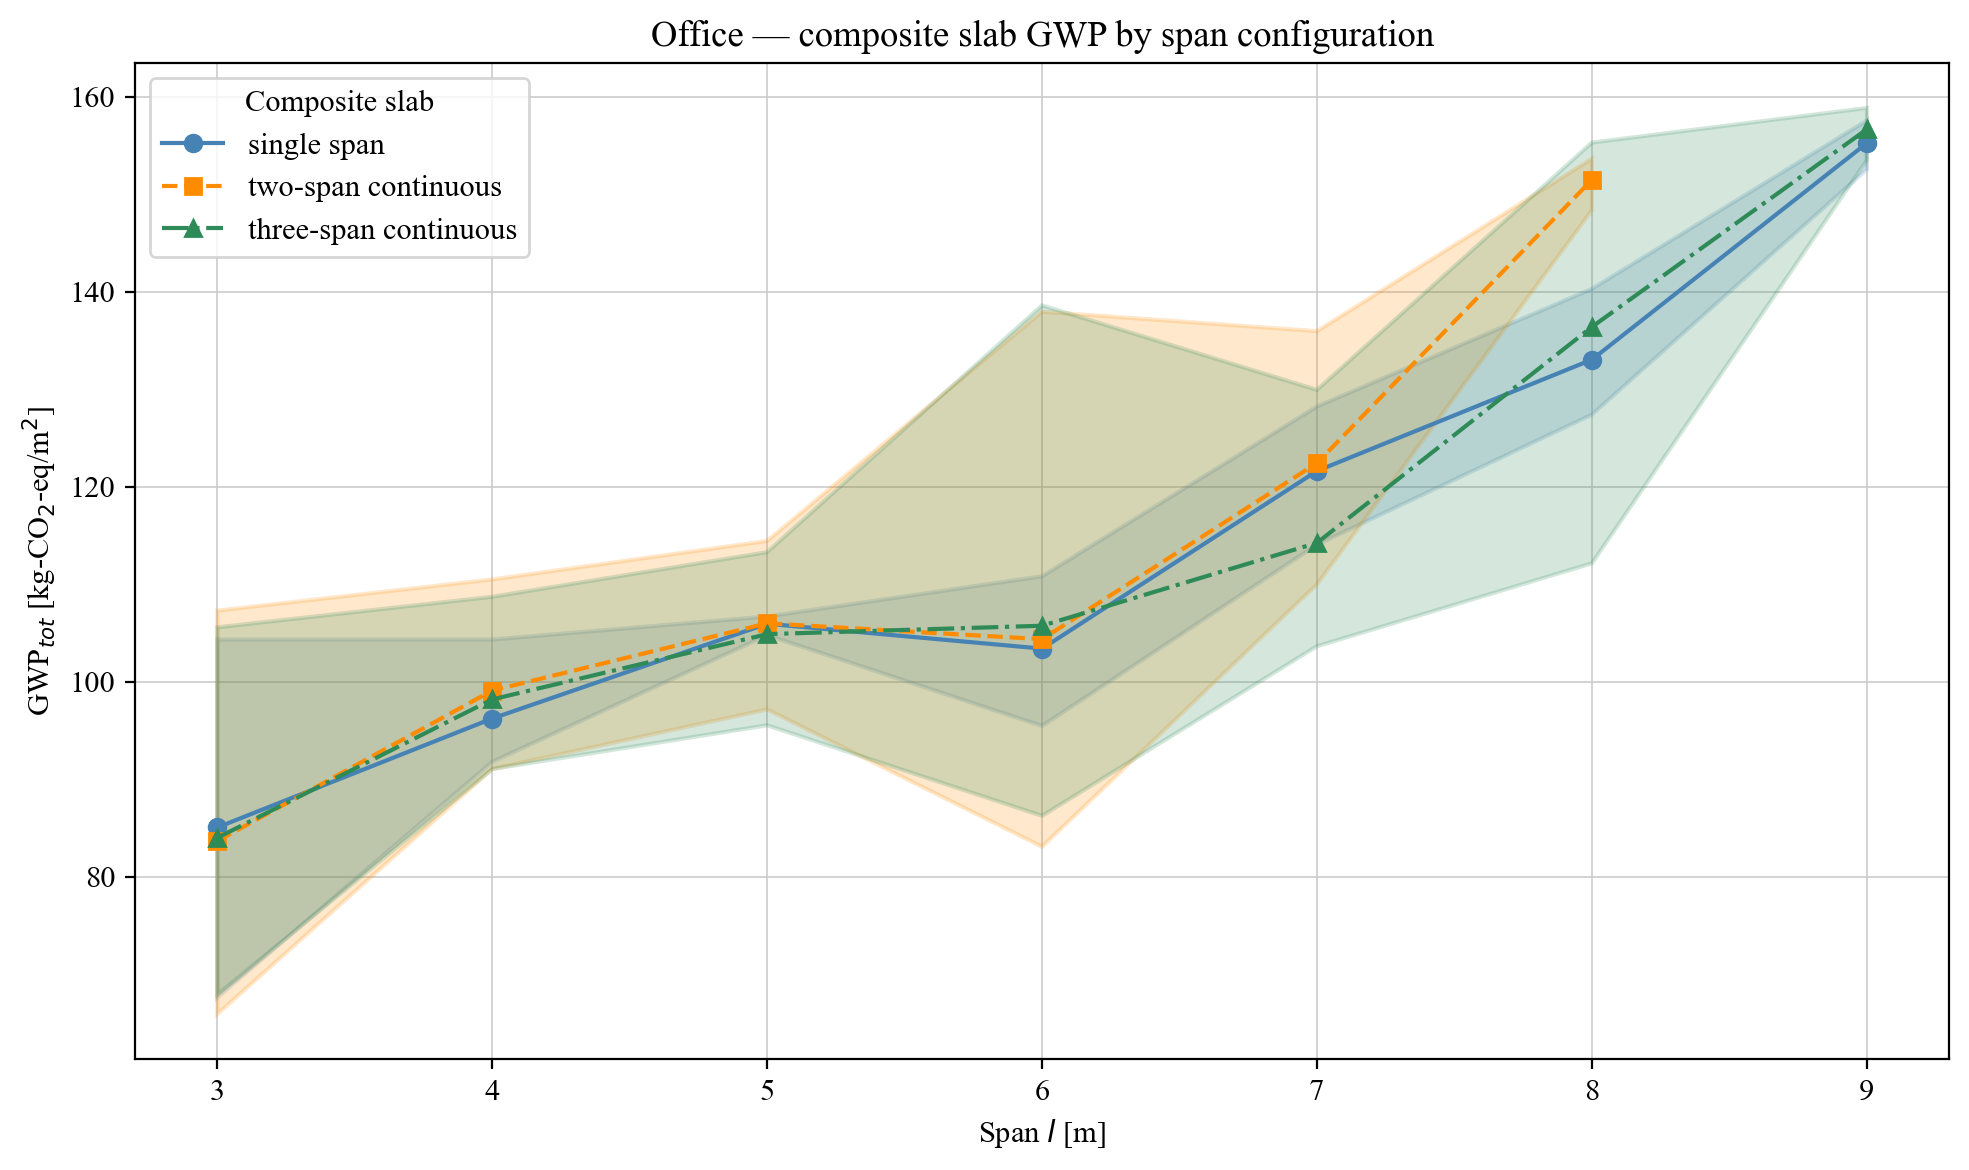
\includegraphics[width=0.85\textwidth]{figures/fig_composite_span_configs.png}
    \caption[Office composite GWP by span configuration]{Office composite slab: total GWP versus span for the single--, two--, and three--span configurations. Shaded bands show the spread of feasible solutions at each span; markers are the GWP optima.}
    \label{fig:office_continuity}
\end{figure}

Up to 6\,m the three configurations are almost indistinguishable: the optima differ by at most a few kg\,CO$_2$eq/m$^2$, and their feasibility envelopes overlap almost completely. The configuration effect emerges only at the longer spans: at 8\,m the three--span optimum (112.1) is the lowest, the single span (127.4) is intermediate, and the two--span case is the highest at 148.4\,kg\,CO$_2$eq/m$^2$ ---higher than the single span, despite being continuous. The two--span configuration also becomes infeasible beyond 8\,m, whereas the single-- and three--span cases reach 9\,m and converge there at around 152--154\,kg\,CO$_2$eq/m$^2$.

%==============================================================================
\subsection{Other occupancy scenarios}
\label{sec:res_other}
%==============================================================================
The residential, retail, and industrial scenarios reproduce the office findings: the composite slab is the highest--carbon system at every span, the ranking of the five systems is unchanged, and the composite design is stiffness-- or hogging--governed over most of the range. Only the differences from the office case are reported here; full figures and tables are in Appendix~\ref{app:results_figures}.

\subsubsection{Residential}
\label{sec:res_residential}
The residential scenario carries a higher imposed load ($q_k = 2.0$\,kN/m$^2$) and a heavier screed-based build-up (+26.4\,kg\,CO$_2$eq/m$^2$), raising all systems' GWP relative to office. The optimal composite cross-sections are listed in Table~\ref{tab:residential_optima}. The single-span composite optimum runs from 80.2 at 3\,m to 165.8\,kg\,CO$_2$eq/m$^2$ at 9\,m; no feasible solution exists at 10\,m. The ranking across the five systems and the governing limit states are unchanged from the office case. Fire D1 governs at 3\,m, fire checks (D2--D4) govern at 4--5\,m, and SLS deflection or hogging governs from 6\,m upward. The composite-to-RC-ribbed gap is again roughly 45\% at short spans, widening with span.

\begin{table}[h!]
\small\centering
\caption{Optimal composite cross--sections, residential scenario, all span configurations.}
\label{tab:residential_optima}
\begin{tabular}{llcccccl}
\toprule
Config. & $L$ [m] & Deck & Grade & $h$ [mm] & $\mathrm{GWP}_\mathrm{tot}$ & Propped & Governing check \\
\midrule
\multirow{7}{*}{Single}
 & 3 & Multideck 80 1.1  & C25/30 & 131 & 80.2  & No  & Fire D1 \\
 & 4 & ComFlor 210       & C25/30 & 290 & 101.5 & No  & Fire D4 \\
 & 5 & ComFlor 60 0.9    & C25/30 & 200 & 97.0  & Yes & Fire D2 \\
 & 6 & ComFlor 210       & C25/30 & 319 & 109.2 & Yes & SLS deflection \\
 & 7 & ComFlor 225       & C25/30 & 392 & 128.5 & Yes & SLS deflection \\
 & 8 & ComFlor 225       & C25/30 & 463 & 142.0 & Yes & ULS long.\ shear \\
 & 9 & Multideck 146 1.5 & C25/30 & 406 & 165.8 & Yes & SLS deflection \\
\midrule
\multirow{6}{*}{Two--span}
 & 3 & Multideck 80 1.0  & C25/30 & 140 & 79.7  & No  & Fire D3 \\
 & 4 & ComFlor 210       & C25/30 & 307 & 104.3 & No  & Fire D2 \\
 & 5 & ComFlor 225       & C25/30 & 313 & 110.3 & No  & Fire D3 \\
 & 6 & ComFlor 60 1.0    & C25/30 & 184 & 101.4 & Yes & ULS hogging \\
 & 7 & ComFlor 210       & C25/30 & 392 & 125.1 & Yes & Fire D3 \\
 & 8 & Multideck 146 1.5 & C25/30 & 448 & 166.7 & Yes & ULS hogging \\
\midrule
\multirow{6}{*}{Three--span}
 & 3 & Multideck 80 1.0  & C25/30 & 140 & 79.4  & No  & Fire D3 \\
 & 4 & ComFlor 210       & C25/30 & 297 & 102.8 & No  & Fire D3 \\
 & 5 & ComFlor 225       & C25/30 & 302 & 108.0 & No  & Fire D3 \\
 & 6 & ComFlor 60 1.0    & C25/30 & 185 & 101.7 & Yes & ULS hogging \\
 & 7 & ComFlor 210       & C25/30 & 351 & 117.7 & Yes & Fire D3 \\
 & 8 & ComFlor 210       & C25/30 & 403 & 128.9 & Yes & Fire D3 \\
\bottomrule
\end{tabular}
\end{table}

\subsubsection{Retail}
\label{sec:res_retail}
The retail scenario uses the same elevated imposed load ($q_k = 4.0$\,kN/m$^2$) as residential but a lighter parquet-and-board build-up (+19.0\,kg\,CO$_2$eq/m$^2$). The optimal cross-sections are listed in Table~\ref{tab:retail_optima}. The single-span composite optimum runs from 70.6 at 3\,m to 156.3\,kg\,CO$_2$eq/m$^2$ at 9\,m. Governing limit states follow the office and residential pattern: fire governs at short spans, SLS deflection or hogging from 6\,m upward. The two-span configuration becomes infeasible beyond 7\,m (one span earlier than the office case), because the higher imposed load increases the hogging demand at the single internal support. The three-span configuration remains feasible to 8\,m.

\begin{table}[h!]
\small\centering
\caption{Optimal composite cross--sections, retail scenario, all span configurations.}
\label{tab:retail_optima}
\begin{tabular}{llcccccl}
\toprule
Config. & $L$ [m] & Deck & Grade & $h$ [mm] & $\mathrm{GWP}_\mathrm{tot}$ & Propped & Governing check \\
\midrule
\multirow{7}{*}{Single}
 & 3 & Multideck 80 1.0  & C25/30 & 131 & 70.6  & No  & Fire D1 \\
 & 4 & ComFlor 210       & C25/30 & 290 & 94.7  & No  & Fire D4 \\
 & 5 & Multideck 146 1.5 & C25/30 & 212 & 107.7 & No  & Fire D4 \\
 & 6 & ComFlor 210       & C25/30 & 309 & 100.5 & Yes & SLS deflection \\
 & 7 & ComFlor 225       & C25/30 & 380 & 119.5 & Yes & SLS deflection \\
 & 8 & Multideck 146 1.2 & C25/30 & 408 & 147.1 & Yes & ULS long.\ shear \\
 & 9 & Multideck 146 1.5 & C25/30 & 392 & 156.3 & Yes & SLS deflection \\
\midrule
\multirow{5}{*}{Two--span}
 & 3 & Multideck 80 1.0  & C25/30 & 139 & 80.4  & No  & Fire D3 \\
 & 4 & ComFlor 210       & C25/30 & 321 & 107.7 & No  & Fire D3 \\
 & 5 & ComFlor 60 0.9    & C25/30 & 166 & 92.9  & Yes & ULS hogging \\
 & 6 & ComFlor 60 1.0    & C30/37 & 206 & 107.9 & Yes & ULS hogging \\
 & 7 & ComFlor 210       & C25/30 & 431 & 133.0 & Yes & ULS hogging \\
\midrule
\multirow{6}{*}{Three--span}
 & 3 & Multideck 80 1.0  & C25/30 & 133 & 79.2  & No  & Fire D3 \\
 & 4 & ComFlor 210       & C25/30 & 307 & 105.0 & No  & Fire D3 \\
 & 5 & ComFlor 60 0.9    & C25/30 & 159 & 91.6  & Yes & ULS hogging \\
 & 6 & ComFlor 80 0.9    & C25/30 & 205 & 104.3 & Yes & ULS hogging \\
 & 7 & ComFlor 210       & C25/30 & 378 & 123.0 & Yes & Fire D3 \\
 & 8 & Multideck 146 1.5 & C25/30 & 407 & 163.0 & Yes & ULS hogging \\
\bottomrule
\end{tabular}
\end{table}

\subsubsection{Industrial}
\label{sec:res_industrial}
The industrial scenario carries the highest imposed load ($q_k = 7.5$\,kN/m$^2$). The optimal cross-sections for all three configurations are listed in Table~\ref{tab:industrial_optima}. Composite GWP is the highest of any scenario, from 92.0 at 3\,m to 173.2\,kg\,CO$_2$eq/m$^2$ at 9\,m (single span). The two-span configuration is feasible at spans of 3--7\,m; hogging governs throughout, transitioning from the fire D3 reduced-section check at 3\,m to composite ULS hogging at 4--7\,m. Beyond 7\,m the elevated imposed load and associated support moment render no deck--reinforcement combination within the depth bound feasible. The three-span configuration shows the same upper limit of 7\,m, again governed by D3 or ULS hogging at the internal supports. Under industrial loading the composite slab's continuous-span range is therefore considerably shorter than in the office scenario, with neither multi-span configuration reaching beyond 7\,m.

\begin{table}[h!]
\small\centering
\caption{Optimal composite cross--sections, industrial scenario, all span configurations.}
\label{tab:industrial_optima}
\begin{tabular}{llcccccl}
\toprule
Config. & $L$ [m] & Deck & Grade & $h$ [mm] & $\mathrm{GWP}_\mathrm{tot}$ & Propped & Governing check \\
\midrule
\multirow{7}{*}{Single}
 & 3 & ComFlor 210       & C25/30 & 290 & 92.0  & No  & Fire D4 \\
 & 4 & ComFlor 210       & C25/30 & 290 & 92.4  & No  & Fire D4 \\
 & 5 & ComFlor 60 0.9    & C25/30 & 211 & 95.4  & Yes & SLS deflection \\
 & 6 & ComFlor 80 1.2    & C25/30 & 261 & 116.4 & Yes & SLS deflection \\
 & 7 & Multideck 146 1.5 & C25/30 & 327 & 141.1 & Yes & SLS deflection \\
 & 8 & Multideck 146 1.5 & C25/30 & 382 & 151.6 & Yes & SLS deflection \\
 & 9 & Multideck 146 1.5 & C30/37 & 430 & 173.2 & Yes & SLS deflection \\
\midrule
\multirow{5}{*}{Two--span}
 & 3 & Multideck 80 1.0  & C25/30 & 154 & 74.4  & No  & Fire D3 \\
 & 4 & ComFlor 60 0.9    & C25/30 & 161 & 82.3  & Yes & ULS hogging \\
 & 5 & ComFlor 60 0.9    & C25/30 & 204 & 90.7  & Yes & ULS hogging \\
 & 6 & ComFlor 80 1.2    & C25/30 & 292 & 121.3 & Yes & ULS hogging \\
 & 7 & Multideck 146 1.5 & C25/30 & 489 & 169.2 & Yes & ULS hogging \\
\midrule
\multirow{5}{*}{Three--span}
 & 3 & Multideck 80 1.1  & C25/30 & 151 & 76.0  & No  & Fire D3 \\
 & 4 & ComFlor 210       & C25/30 & 313 & 97.7  & No  & Fire D3 \\
 & 5 & ComFlor 60 0.9    & C25/30 & 179 & 87.5  & Yes & ULS hogging \\
 & 6 & ComFlor 210       & C25/30 & 379 & 113.7 & Yes & Fire D3 \\
 & 7 & Multideck 146 1.5 & C25/30 & 406 & 153.3 & Yes & Fire D3 \\
\bottomrule
\end{tabular}
\end{table}

%==============================================================================
\subsection{Cross-scenario comparison}
\label{sec:res_cross}
%==============================================================================
\begin{figure}[h!]
    \centering
    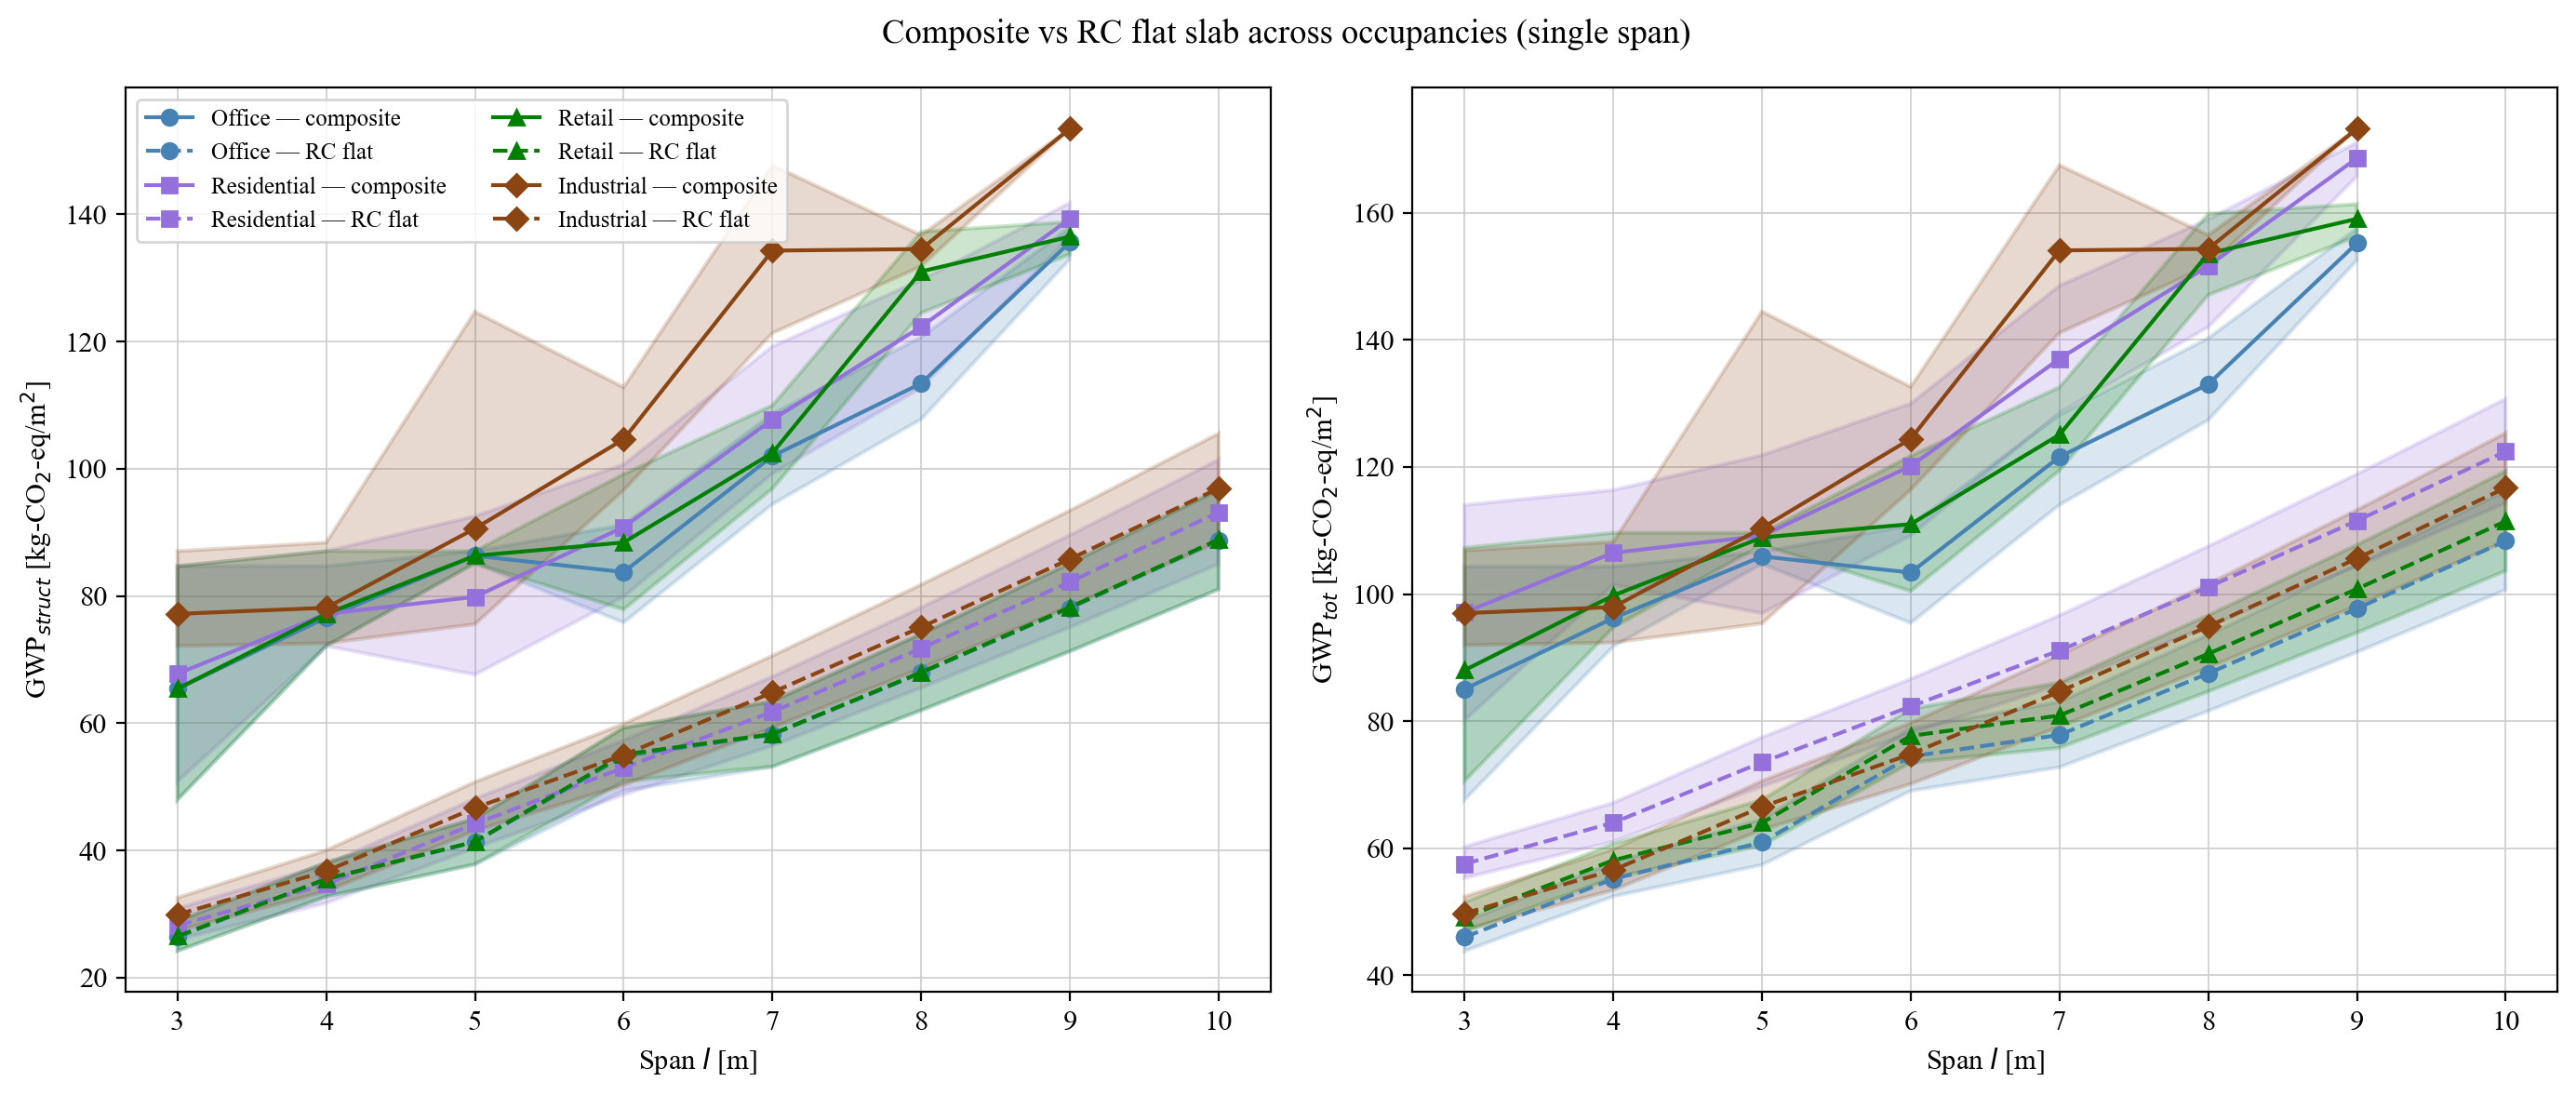
\includegraphics[width=0.9\textwidth]{figures/fig_composite_vs_rc_occupancies.png}
    \caption[Composite versus RC flat across occupancies]{Total GWP versus span for the composite slab (solid) and RC flat slab (dashed) in all four occupancy scenarios, single span.}
    \label{fig:cross_scenario}
\end{figure}

Across all four occupancies the composite slab is the highest--carbon system and the ranking of the five systems is preserved. The absolute GWP scales with imposed load and build--up mass (industrial highest, office lowest), but the \emph{relative} position of the composite slab does not change. The composite--to--RC--flat gap is narrowest for office (the lightest loading) and widest for industrial, indicating that the carbon disadvantage of composite construction grows with imposed load.

%==============================================================================
\subsection{Building-envelope comparison}
\label{sec:res_envelope}
%==============================================================================
The per-unit-area comparisons above treat each floor system in isolation. At the scale of a whole building, however, the structural depth of the floor has a further consequence: for a fixed overall building height, a shallower floor-to-floor construction depth allows more storeys to be accommodated, and hence more lettable or usable floor area. This building-envelope analysis translates the structural depth results into an achievable storey count, providing a building-level perspective that the per-square-metre GWP comparison does not capture.

For each slab system, span, and span configuration, the floor-to-floor height was computed as the sum of the clear storey height, the structural slab depth $h$ (the minimum-GWP section from the optimisation), and a fixed ceiling/services void. The achievable storey count is then the fixed building height divided by this floor-to-floor height. The building parameters assumed for each occupancy are typical values for that use: an office building of 40\,m with 2.7\,m clear height and a 0.40\,m services void; a residential building of 30\,m with 2.5\,m clear height and a 0.20\,m void; a retail building of 20\,m with 4.0\,m clear height and a 0.35\,m void; and an industrial building of 12\,m with 6.0\,m clear height and a 0.25\,m void. The resulting storey counts are continuous; the achievable integer count is the floor of each value. The results are tabulated in Table~\ref{tab:envelope_office_storey}.

\begin{table}[h!]
\centering
\small
\caption{Achievable storey count vs span --- Office (building height = 40\,m, clear height = 2.7\,m, ceiling void = 0.40\,m). Values are continuous; $\lfloor n \rfloor$ gives the achievable integer count.}
\label{tab:envelope_office_storey}
\begin{tabular}{lrrrrrrrr}
\toprule
Slab type & 3\,m & 4\,m & 5\,m & 6\,m & 7\,m & 8\,m & 9\,m & 10\,m \\
\midrule
Composite (SS) & 12.13 & 11.57 & 11.84 & 11.54 & 11.29 & 11.10 & 11.25 & --- \\
Composite (2-span) & 12.13 & 11.57 & 11.55 & 12.00 & 11.33 & 11.21 & --- & --- \\
Composite (3-span) & 12.13 & 11.57 & 11.58 & 11.98 & 11.44 & 11.30 & 11.19 & --- \\
\midrule
RC Solid & 12.26 & 12.06 & 12.05 & 11.87 & 11.84 & 11.71 & 11.59 & 11.45 \\
RC Ribbed & 11.95 & 11.67 & 11.53 & 11.41 & 11.21 & 11.11 & 10.91 & 10.79 \\
Timber Solid & 11.81 & 11.67 & 11.50 & 11.48 & 11.32 & 11.16 & 10.98 & 10.99 \\
Timber Ribbed & 11.21 & 11.21 & 11.12 & 11.05 & 10.82 & 10.49 & 10.29 & 10.07 \\
\bottomrule
\end{tabular}
\end{table}

\begin{figure}[h!]
    \centering
    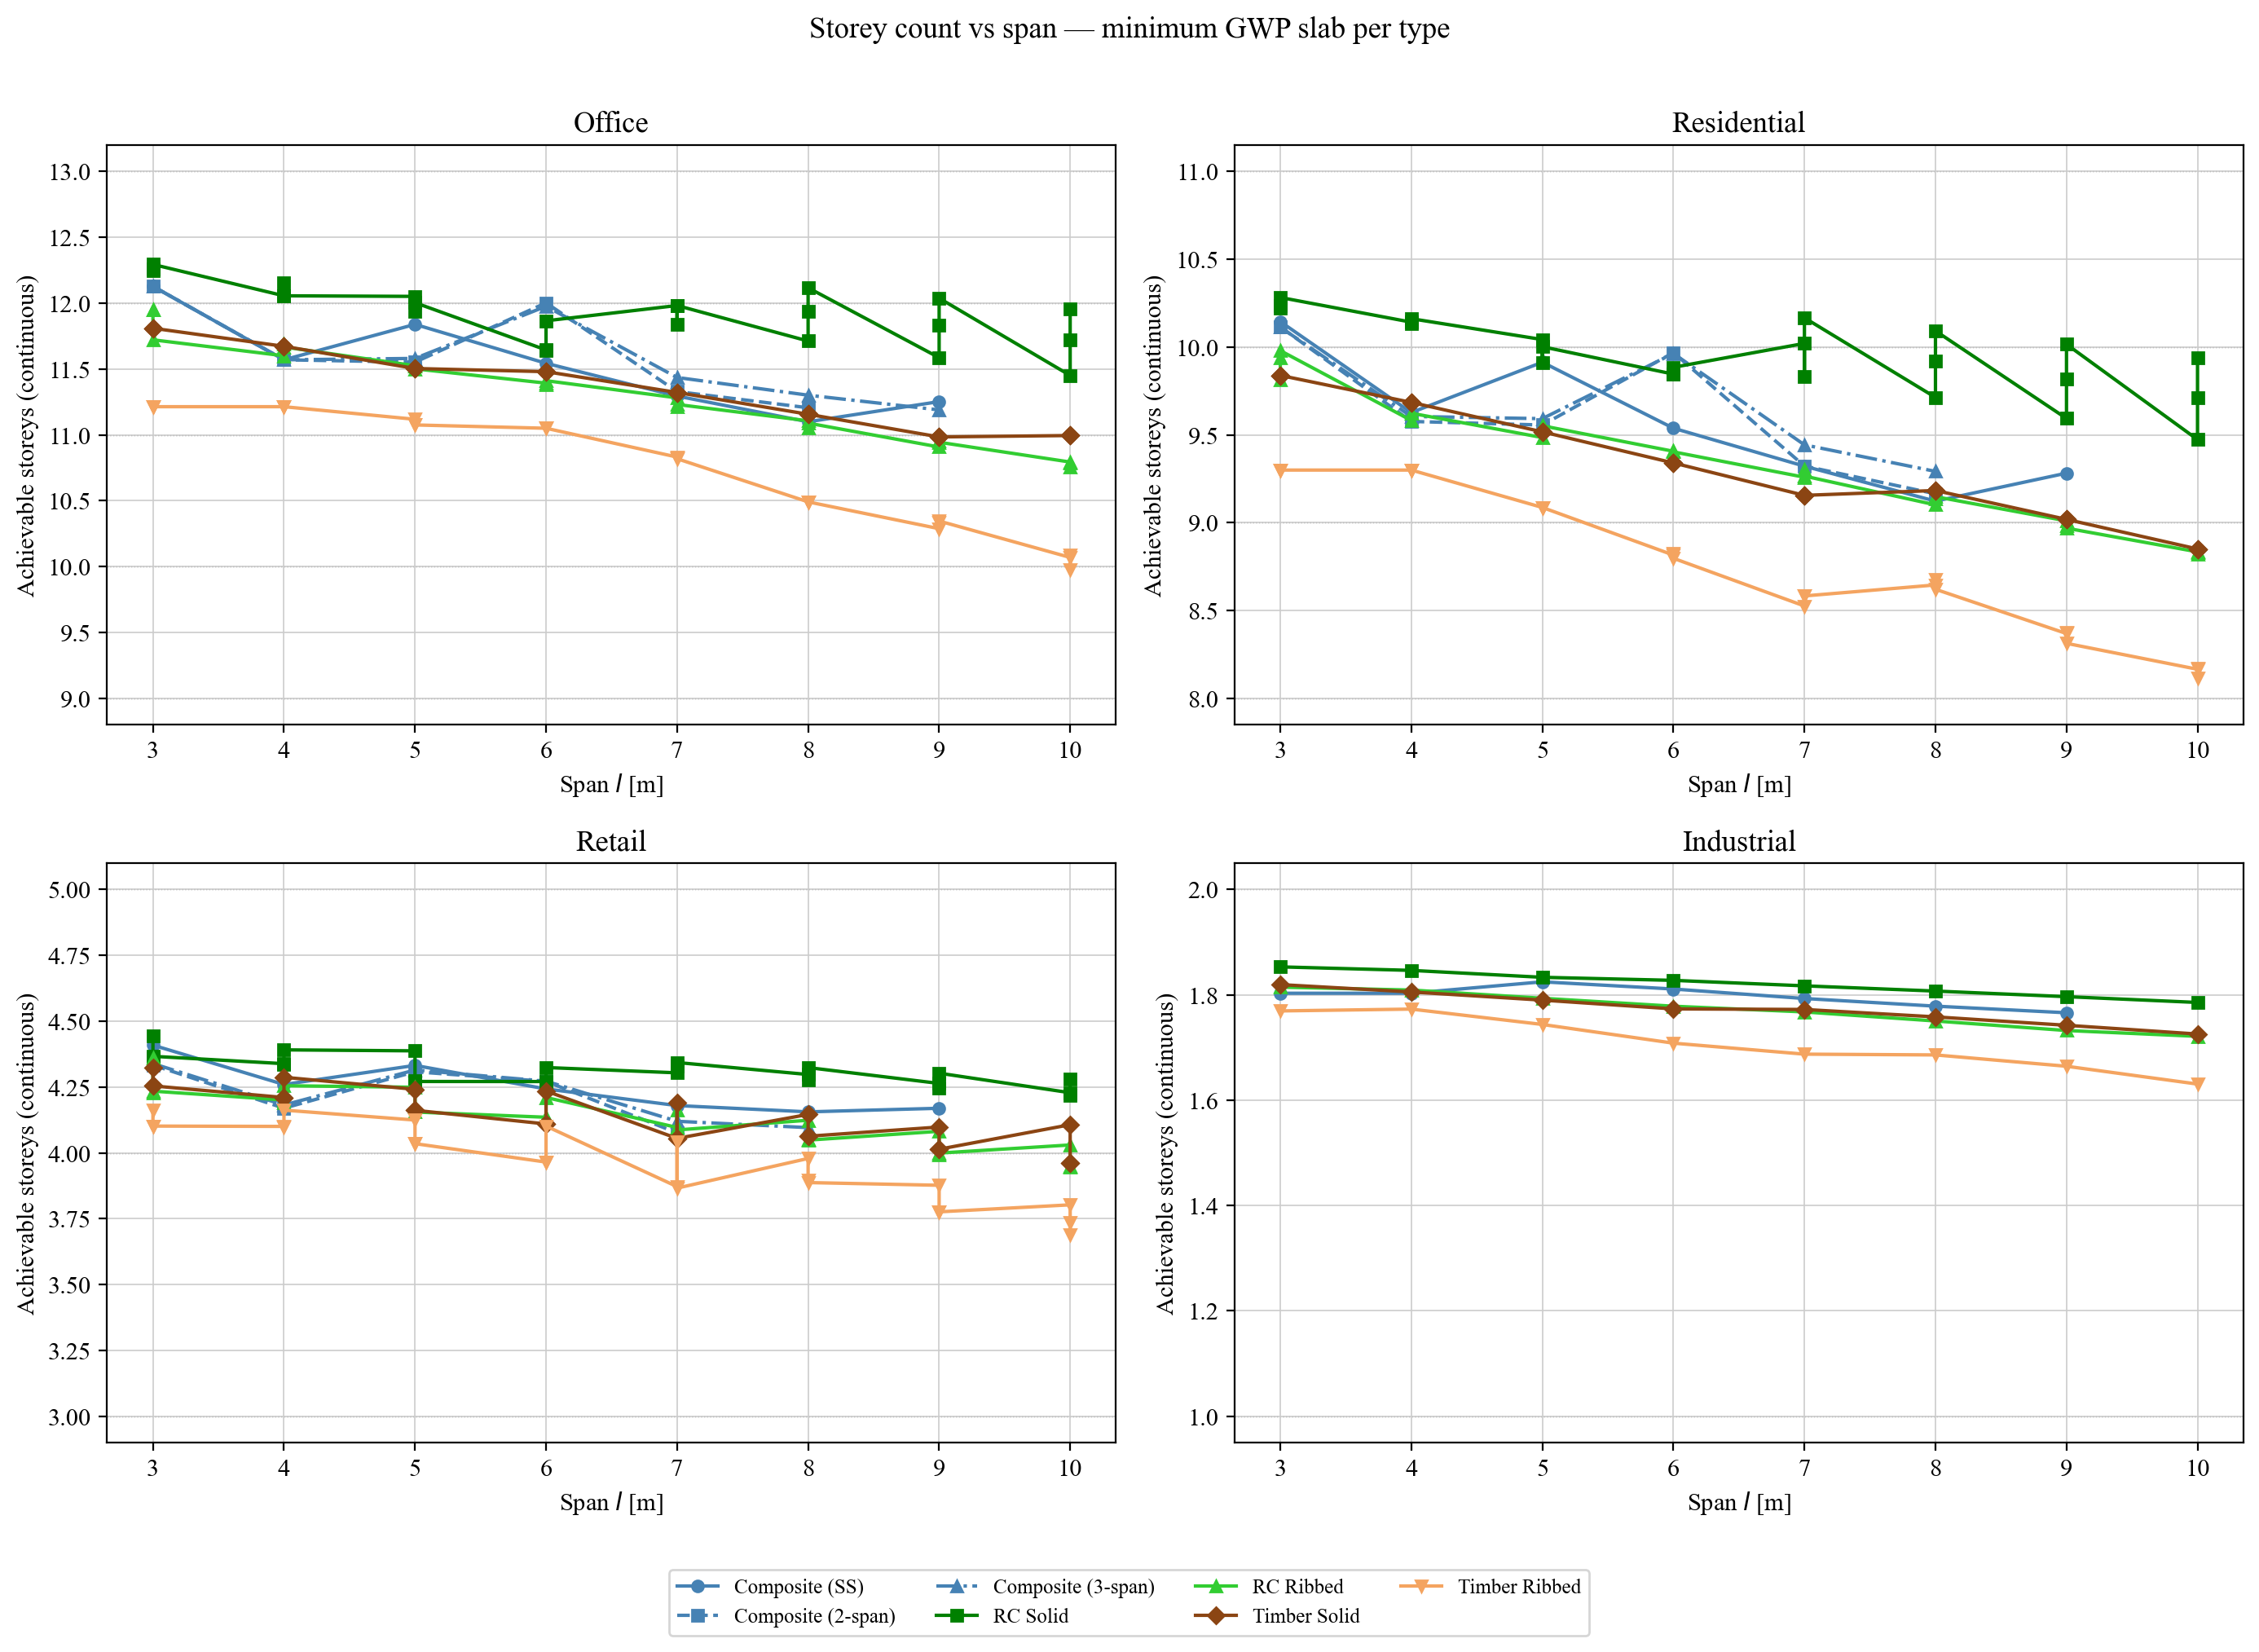
\includegraphics[width=\textwidth]{figures/fig_envelope_storey_count.png}
    \caption[Achievable storey count versus span, all occupancies]{Achievable storey count versus span for the minimum--GWP section of each slab system, across all four occupancy scenarios}
    \label{fig:envelope_storey_count}
\end{figure}

The building-envelope ranking differs markedly from---and is in large part the inverse of---the embodied-carbon ranking. The RC solid (flat) slab, being the shallowest structural section across almost the entire span range, achieves the highest storey count in every occupancy. The composite slab ranks second at short spans (for example 12.13 achievable storeys at 3\,m office, against 12.26 for RC solid) but falls back towards the middle at longer spans, where its deep-deck sections increase the floor-to-floor height. Critically, the two systems that performed best on embodied carbon---the timber rectangular and RC ribbed slabs---perform worst on storey count, because their greater structural depth consumes more of the building height per floor. The timber ribbed slab, with the deepest sections, achieves the fewest storeys throughout.

This result reframes the headline finding of this chapter. On embodied carbon alone the composite slab is the least favourable system (Section~\ref{sec:res_office_gwp}); on building-height efficiency it is among the best, second only to the RC flat slab and well ahead of the low-carbon timber and ribbed systems. The depth-competitiveness of the composite slab---its ability to deliver nearly as many storeys as the RC flat slab---is one of the practical advantages that offsets its higher embodied carbon, and is examined further in the discussion (Chapter~\ref{fifthchapter}).

%==============================================================================
\subsection{Validation against manufacturer tables}
\label{sec:res_validation}
%==============================================================================
To establish confidence in the structural model, the maximum permissible span computed by the optimiser for each deck was compared against the manufacturer's published load/span tables. For every deck profile and gauge for multispan decks, the model's design span was expressed as a ratio of the manufacturer's tabulated maximum span for the equivalent loading; a ratio at or below unity indicates that the model design lies within the manufacturer's envelope. Comparisons were made against both British Standard and Eurocode manufacturer tables as available, at an imposed load of 5 or 6\,kN/m$^2$ depending on the tables used.

Of the 406 deck--span--configuration combinations checked, 103 had no comparable manufacturer table (chiefly propped cases for which no propped table is published) and were excluded. Of the 303 comparable checks, 266 (87.8\,\%) passed, and---importantly---every passing case lies within the manufacturer envelope (span ratio $\leq 1.0$, mean 0.78). The model is therefore consistently conservative relative to the published tables. Table~\ref{tab:verification} summarises the outcome by deck family and Figure~\ref{fig:verification} shows the span-ratio distribution for every deck.

\begin{table}[h!]
\small\centering
\caption{Verification against manufacturer load/span tables, by deck family. ``Comparable'' excludes cases with no published table.}
\label{tab:verification}
\begin{tabular}{lcccc}
\toprule
Deck family & Comparable & Pass & Fail & Pass rate \\
\midrule
ComFlor 46  & 6   & 6   & 0  & 100\,\% \\
ComFlor 51  & 42  & 39  & 3  & 93\,\% \\
ComFlor 60  & 56  & 42  & 14 & 75\,\% \\
ComFlor 80  & 43  & 34  & 9  & 79\,\% \\
ComFlor 210 & 25  & 16  & 9  & 64\,\% \\
ComFlor 225 & 27  & 25  & 2  & 93\,\% \\
Multideck 60  & 33 & 33 & 0 & 100\,\% \\
Multideck 80  & 30 & 30 & 0 & 100\,\% \\
Multideck 146 & 41 & 41 & 0 & 100\,\% \\
\midrule
\textbf{Total} & \textbf{303} & \textbf{266} & \textbf{37} & \textbf{87.8\,\%} \\
\bottomrule
\end{tabular}
\end{table}

\begin{figure}[h!]
    \centering
    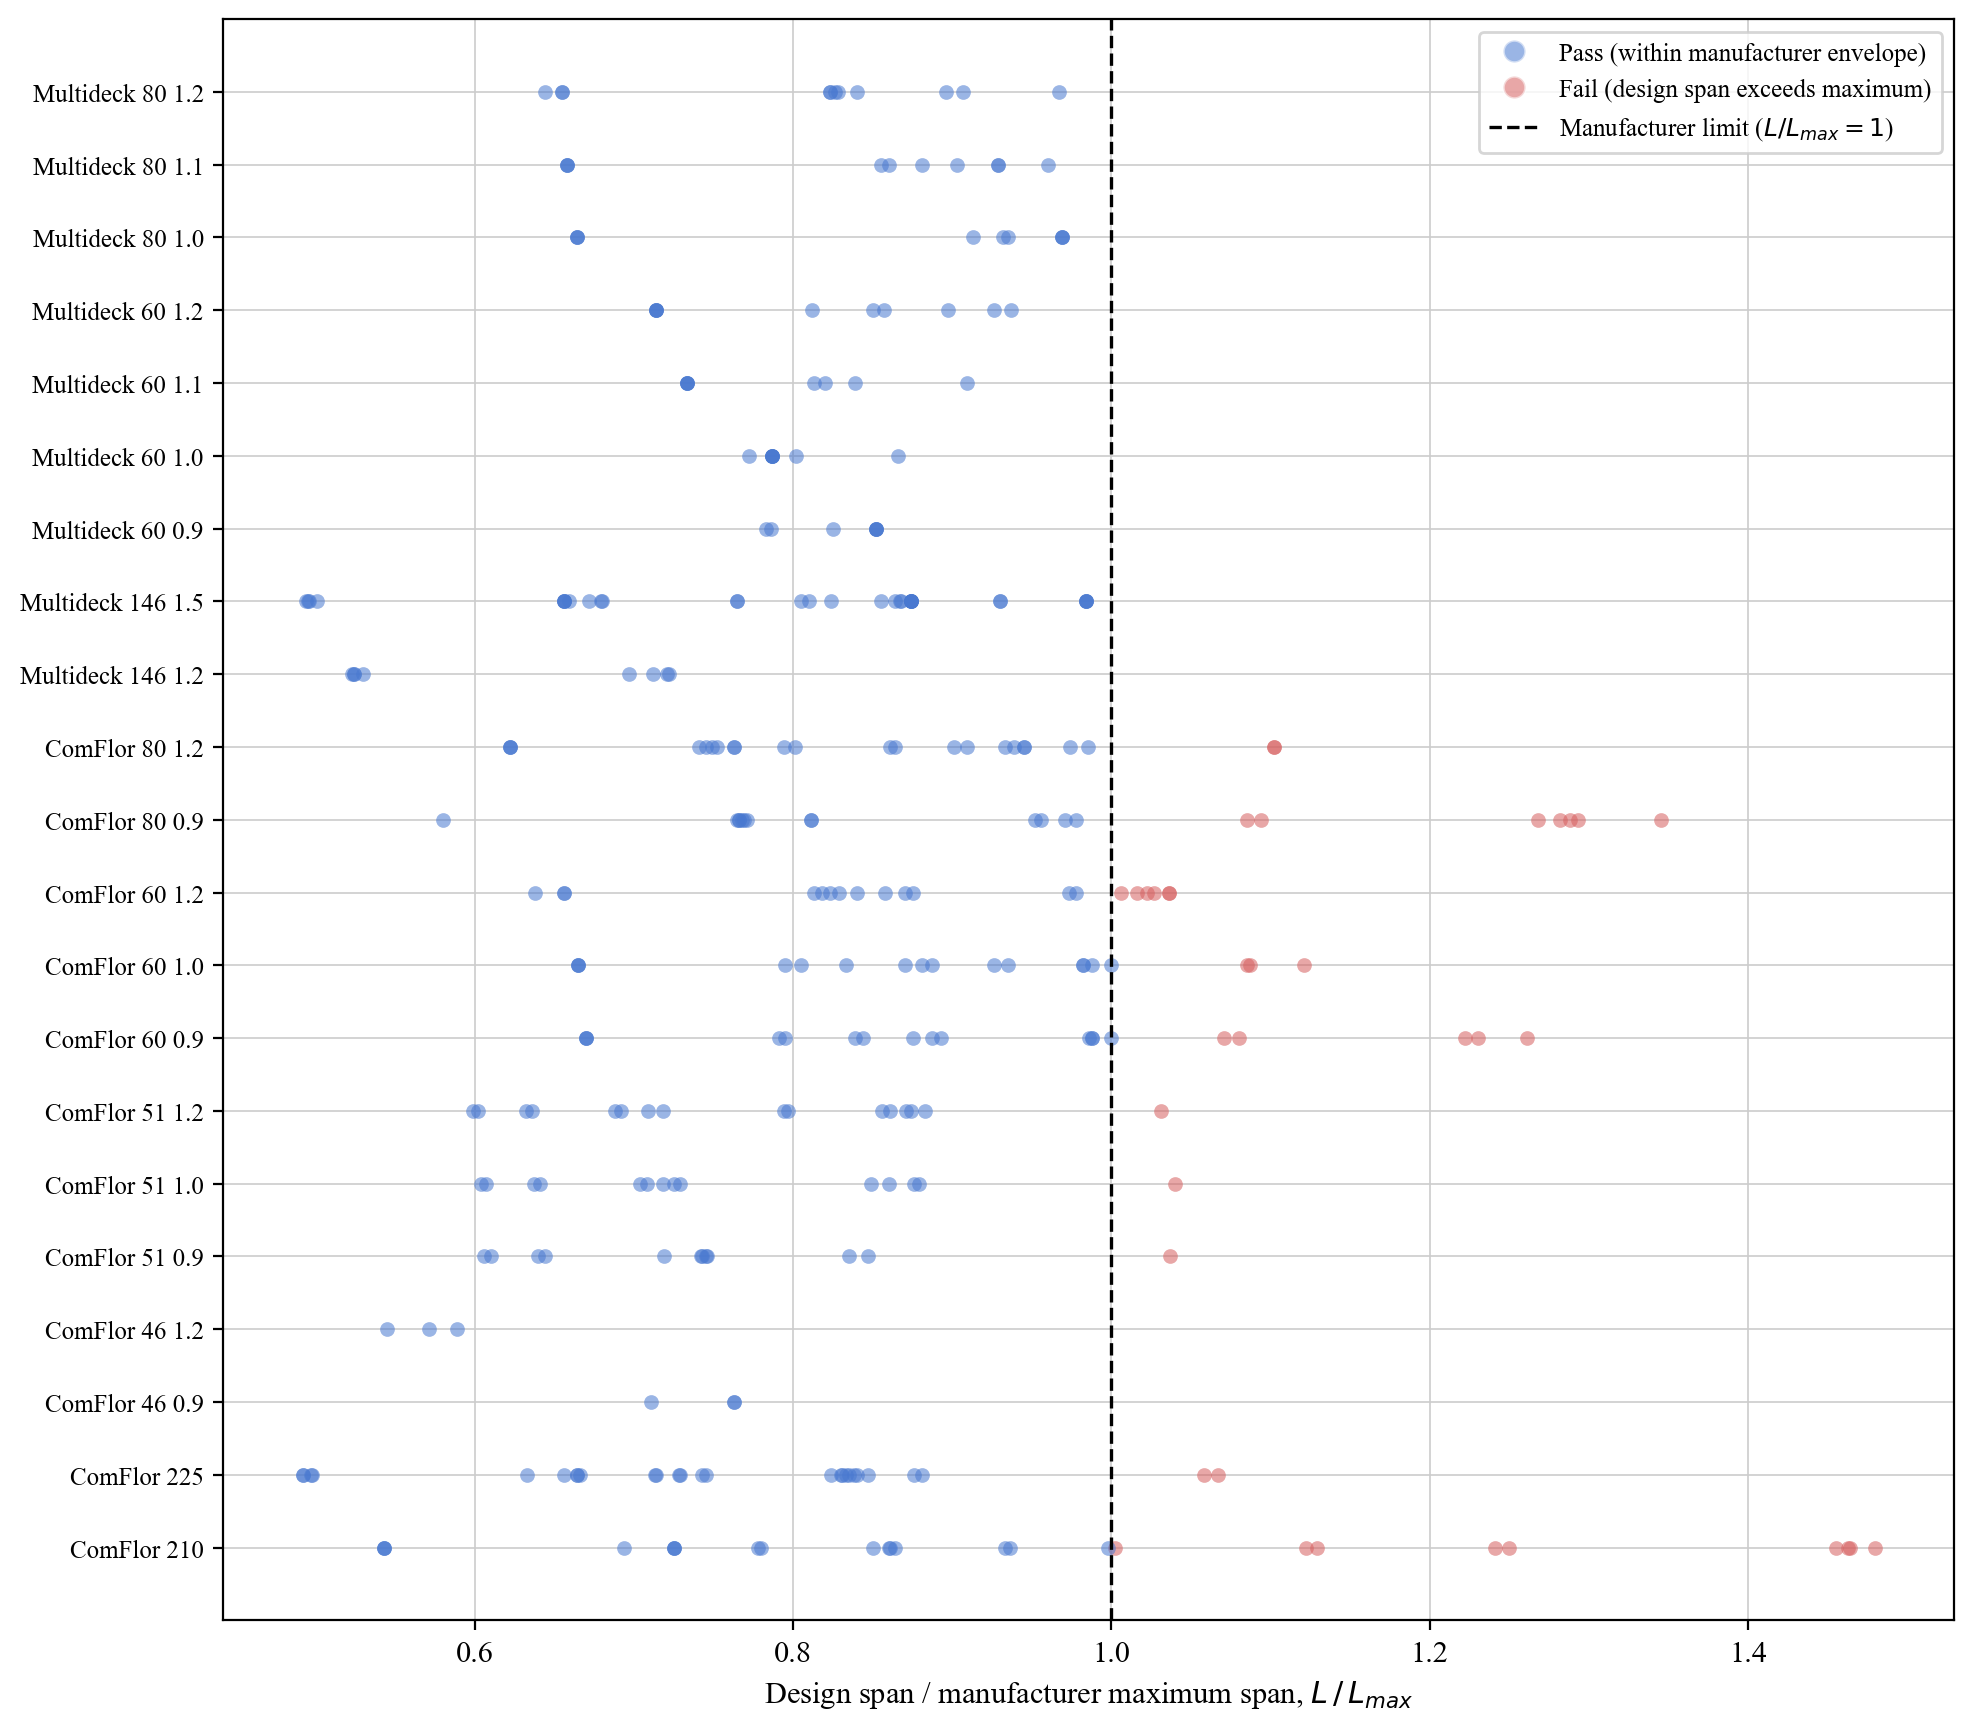
\includegraphics[width=0.95\textwidth]{figures/fig_mfr_verification.png}
    \caption[Model span versus manufacturer maximum]{Design span as a fraction of the manufacturer's published maximum span, for every deck profile and gauge.}
    \label{fig:verification}
\end{figure}

All 37 failures share two features: they are all propped cases, and all occur where the model's design span only marginally exceeds the manufacturer's tabulated maximum (span ratio just above unity, for example ComFlor 60 0.9 at 5\,m against a published maximum of 4.63\,m). They are concentrated in the deeper ComFlor profiles (210, 80, 60) at their longest spans, and are more frequent for the Eurocode-based tables (17\,\% fail) than the British Standard tables (7\,\%) and for the three-span configuration. The Multideck range passes without exception. Since these marginal cases sit at the limit of each deck's span range and the optimiser does not select them as GWP optima, the verification gives good confidence in the structural model across the span range relevant to the results.

%==============================================================================
\subsection{Summary}
\label{sec:res_summary}
%==============================================================================
The central result of this study is consistent across all four occupancy scenarios, all three span configurations, and the full practical span range: the composite steel--concrete slab carries the highest embodied carbon of the five floor systems compared, exceeding the RC flat baseline by a margin that widens with both span and imposed load, and exceeding the RC ribbed and timber systems by even larger margins. The composite design is governed by SLS deflection (single span) or by hogging at internal supports (continuous spans) over most of the range, with fire and longitudinal shear governing only at the shortest spans; it requires propped construction at spans over 5\,m for the office range and, under industrial loading, reaches at most 7\,m in both the two-- and three--span configurations. These findings answer the primary research question directly---on embodied carbon alone, the composite slab does not offer an advantage over reinforced concrete flat slabs---and motivate the discussion in Chapter~\ref{fifthchapter}, where the non--carbon considerations that nonetheless favour composite construction (construction speed, structural depth, service integration, and cost) are examined.

    \section{Discussion}
\label{fifthchapter}

This chapter interprets the results presented in Chapter~\ref{fourthchapter} and situates them within the broader context of sustainable structural design. It first addresses the central finding: that the composite slab carries the highest embodied carbon of the systems compared, yet composite construction remains widely specified in practice. It then examines the behaviour within and between slab systems, compares the results against the published literature, considers the validity and limitations of the design methodology, and identifies directions for further work.

%==============================================================================
\subsection{Why composite slabs are used despite higher GWP}
\label{sec:disc_why_composite}
%==============================================================================
The results show unambiguously that, on embodied carbon alone, the composite slab is the least favourable of the five systems across every span, occupancy, and span configuration (Section~\ref{sec:res_office_gwp}). This raises the obvious question of why composite steel--concrete floors are nonetheless among the most common floor systems in multi-storey steel-framed construction. The answer lies in the factors that an embodied-carbon comparison does not capture, and which a designer weighs alongside it.

\paragraph{Construction speed and programme.} Profiled steel decking acts as permanent formwork and a working platform, eliminating the need for temporary formwork and allowing rapid floor-by-floor construction. The deck can be lifted in stacks and laid out quickly, providing an immediate safe working surface for following steps. Because labour is now the dominant cost in many markets, this programme saving translates directly into lower construction cost, and the faster cycle time can bring forward a building's revenue or occupation date---commercial advantages that a per-square-metre embodied-carbon figure does not register. The trade-off identified in this study is that unpropped construction, which preserves this speed advantage in full, is feasible only up to 5\,m in the office range (Section~\ref{sec:res_office_gov}); at longer spans the programme benefit is negated by the need for temporary propping.

\paragraph{Self-weight and foundation demand.} Although the composite slab is heavier than the timber systems, it is lighter than a solid RC flat slab of equivalent span for much of the range, which reduces column and foundation loads and the seismic mass of the structure. In tall buildings this cumulative weight saving can be decisive and is not reflected in a per-floor GWP figure.

\paragraph{Structural depth and service integration.} On structural depth the composite slab is competitive despite its high embodied carbon. At the longest feasible spans its total depth is the second-shallowest of the five systems, exceeded only by the RC flat slab and sitting well below the RC ribbed and both timber systems (Section~\ref{sec:res_office_depth}). This depth-competitiveness carries through to the building scale: in the storey-count analysis (Section~\ref{sec:res_envelope}) the composite slab achieves the second-highest achievable storey count for a fixed building height, behind only the RC flat slab and ahead of the two lowest-carbon systems (RC ribbed and timber rectangular), which are penalised by their greater structural depth. For a fixed overall building height, a shallower floor-to-floor construction depth allows either more lettable storeys or, equivalently, a lower total building height for a fixed storey count---reducing cladding area and the embodied carbon of columns, cores, and foundations across the whole structure. A saving of this kind acts at the building level rather than the floor level and is therefore not clear in the per-square-metre slab comparison that places composite last. The deep-deck profiles selected at longer spans also create voids through which services can be routed, and in steel-framed construction services are commonly passed through cellular-beam web openings, further reducing the floor-zone depth relative to a downstand-beam arrangement. The depth advantage is, however, not seen at the longest composite spans, where the abrupt transition to a deep deck (Section~\ref{sec:res_office_depth}) increases the floor-to-floor height and pulls the composite storey count back towards the middle of the ranking.

\paragraph{Demountability and material recovery.} Steel decking and beams can in principle be unbolted and reused or recycled at end of life, whereas monolithic RC is typically downcycled to aggregate. The embodied-carbon accounting in this study is a cradle-to-gate (A1--A3) and transport (C) boundary and therefore does not credit end-of-life recovery, which would partially close the gap to the RC systems.

%==============================================================================
\subsection{Behaviour within the composite slab system}
\label{sec:disc_within}
%==============================================================================
\paragraph{Governing limit states.} The composite slab is stiffness-governed rather than strength-governed over most of the practical range: SLS deflection controls the single-span optima from 5\,m upward, and the hogging checks control the continuous configurations (Section~\ref{sec:res_office_gov}). This has a direct GWP consequence---additional depth and material are being added to satisfy a serviceability limit, not to carry load---and explains why the optimum is insensitive to concrete grade (C25/30 is selected almost throughout, since a stronger grade adds GWP without adding the stiffness that governs).

\paragraph{Effect of span continuity.} The non-monotonic effect of continuity (Section~\ref{sec:res_office_continuity}) is one of the more nuanced findings. Continuity reduces composite GWP in the intermediate range, where the lower span moments allow a shallow deck to be retained, but penalises it at long spans, where the support hogging moment forces a deeper section. This contrasts with the RC flat slab, which benefits from continuity across the whole range. Figure~\ref{fig:office_continuity} plots the three configurations on a single axis. Up to 6\,m the optima are almost indistinguishable, differing by at most a few kg\,CO\textsubscript{2}eq/m\textsuperscript{2} with their feasibility envelopes overlapping almost completely; the configuration effect emerges only beyond this crossover. At 8\,m the three-span optimum (112.1\,kg\,CO\textsubscript{2}eq/m\textsuperscript{2}) is the lowest envelope value, the single span (127.4) intermediate, and the two-span case the highest at 148.4\,kg\,CO\textsubscript{2}eq/m\textsuperscript{2}--- 21\,kg\,CO\textsubscript{2}eq/m\textsuperscript{2} (roughly 17\,\%) above the single span despite being continuous. The two-span configuration also becomes infeasible beyond 8\,m, because the hogging moment at its single internal support is the most severe of the three arrangements, whereas the three-span case distributes the support moments more favourably and recovers feasibility at 9\,m.

\paragraph{Preferred deck profiles.} The optimiser selects from two distinct families of profile depending on which limit state governs. At short spans, where the section is set by the fire thermal-insulation minimum (D1) rather than by strength or stiffness, a shallow profile is chosen---typically Multideck~80 in the single-span office case and the shallow trapezoidal ComFlor~60 in the continuous configurations, retained for one meter further by the reduced sagging moment over continuous supports. As span increases and the deflection limit (single span) or support hogging check (continuous spans) can no longer be met within a shallow section, the optimiser steps abruptly to a deep profile---ComFlor~210, ComFlor~225, or Multideck~146. The shape of that curve is therefore driven by the availability of discrete deck profiles in the database, not by a continuous trade-off, and the same shallow-then-deep pattern recurs across all four occupancy scenarios, with the transition occurring at progressively shorter spans as the imposed load increases.

%==============================================================================
\subsection{Comparison between slab systems}
\label{sec:disc_between}
%==============================================================================
\paragraph{Ranking and application.} Across all scenarios the GWP ranking is consistent: timber rectangular lowest, then RC ribbed, RC flat, timber ribbed, and composite highest (Section~\ref{sec:res_office_gwp}). The ranking should, however, be read alongside the intended application of each system, since each occupies a distinct niche in practice and a higher-carbon system is not simply discarded on that basis alone. Table~\ref{tab:slab_applications} summarises the typical use cases. The composite slab's position as the highest-carbon system must therefore be weighed against its established role in fast-track, long-span, steel-framed construction, where its non-carbon attributes (Section~\ref{sec:disc_why_composite}) are decisive.

\begin{table}[h!]
\centering
\caption{Typical application niches of the five floor systems compared.}
\label{tab:slab_applications}
\small
\begin{tabular}{p{0.22\textwidth} p{0.70\textwidth}}
\hline
System & Typical application \\
\hline
Timber rectangular & Low- to medium-rise residential and education; sustainability-led projects; sites with low fire and acoustic demand or where a lightweight superstructure reduces foundation cost \citep{CLT2023}. \\
RC ribbed & Longer-span floors where material efficiency is prioritised; material-efficient but formwork-intensive, so favoured where reuse of moulds offsets the labour cost \citep{RefWorks:kaufmann2024white}. \\
RC flat & The default multi-storey solution: simple flat soffit, flexible layout, unobstructed service routing below the slab, and well-understood construction; chosen for its low cost and buildability rather than minimum material \citep{RefWorks:kaufmann2024white,RefWorks:ammann2024correlations}. \\
Timber ribbed & Engineered-timber long-span floors in sustainability-led commercial and institutional buildings; higher GWP than solid timber owing to the glulam ribs \citep{CLT2023} \\
Composite & Steel-framed multi-storey commercial and office buildings; fast-track construction, long spans, shallow floor zones, and service integration through deep-deck voids or cellular beams \citep{RefWorks:2011composite,RefWorks:ahmed2019evolution,RefWorks:lawson1999slimflor,RefWorks:scip300}. \\
\hline
\end{tabular}
\end{table}

\paragraph{Scope of the comparison.} An important caveat is that only the composite and RC flat systems were extended to continuous spans; the RC ribbed and timber systems are single-span analyses (Section~\ref{sec:res_intro}). The cross-system ranking is therefore most rigorous for the single-span case. For the continuous configurations the comparison is fair between composite and RC flat, the two systems most commonly used continuous in practice, but the ribbed and timber baselines should be read as single-span reference points rather than as fully optimised continuous designs. Extending these systems to continuous spans falls outside the scope of the present work and is being undertaken separately within the research group.

\paragraph{Building-envelope perspective.} The building-envelope analysis (Section~\ref{sec:res_envelope}) reframes the ranking by translating structural depth into an achievable storey count for a fixed building height. At this scale the ranking is in large part the inverse of the embodied-carbon ranking: the RC flat slab, being the shallowest section across almost the entire span range, achieves the highest storey count in every occupancy, while the lowest-carbon systems---the timber and RC ribbed slabs---perform worst, because their greater structural depth consumes more of the building height per floor. The composite slab, last on embodied carbon, ranks second on storey count (for example 12.13 achievable storeys at 3\,m office against 12.26 for the RC flat slab), falling back towards the middle only at the longest spans where its deep-deck sections increase the floor-to-floor height. The two rankings therefore do not agree, and this disagreement is the central qualification on the per-square-metre comparison: a slab judged solely on floor-level GWP can be penalised for a depth efficiency that, at the building scale, allows more usable area or a smaller envelope per storey. The two metrics should be read together: the per-square-metre figure captures the embodied carbon of the floor itself, while the storey-count figure captures the consequential effect of slab depth on the rest of the structure.

%==============================================================================
\subsection{Comparison with the literature}
\label{sec:disc_literature}
%==============================================================================
The central finding is consistent with the work of \cite{RefWorks:regulez2022sustainability}, who compared slab typologies including steel--concrete composites and concluded that the composite slab becomes progressively less efficient than reinforced concrete as span increases (Chapter~\ref{secondchapter}, Figure~\ref{fig:regulez2022}). The present results reproduce this trend and extend it: not only does the composite slab become relatively less efficient with span, it is the highest-carbon option across the entire practical range and all four occupancies, and the divergence is driven specifically by the SLS-deflection-governed deep-deck transition identified in Section~\ref{sec:res_office_depth}.

%==============================================================================
\subsection{Validity and limitations}
\label{sec:disc_method}
%==============================================================================
\paragraph{Verification against manufacturer data.} The verification against published load/span tables (Section~\ref{sec:res_validation}) gives good confidence in the structural model across the span range relevant to the results. Of the 303 comparable deck--span--configuration checks, 266 (87.8\,\%) passed, confirming that the implementation is conservative rather than unconservative. The 37 failures share two features that limit their significance: they are all propped cases (for which no propped manufacturer table exists, so the comparison is against an unpropped maximum), and all occur where the model's design span only marginally exceeds the tabulated maximum, concentrated in the deepest ComFlor profiles at their longest spans. Crucially, the optimiser does not select these marginal sections as GWP optima, so the failures do not affect the reported results. The conservatism is attributable in part to the modelling choices flagged in Section~\ref{sec:assumptions}: the $A_{p,e}=0.9\,A_p$ (shallow) and $0.5\,A_p$ (deep) fallback applied where the manufacturer does not publish an effective area reduces the computed sagging and longitudinal-shear resistances relative to the test-derived values used in manufacturer software, and the omission of end anchorage (Appendix~\ref{app:end_anchorage}) further lowers the longitudinal-shear capacity. The implication for the GWP results is reassuring: because the model is conservative, the composite cross-sections it selects are if anything slightly heavier (and therefore higher-carbon) than a manufacturer would specify.

\paragraph{EPD consistency and the ArcelorMittal exclusion.} The exclusion of ArcelorMittal decking on the grounds of a single-value EPD (Section~\ref{sec:assumptions}) is a methodological strength rather than a gap: it prevents a systematic bias that would have favoured deep composite sections artificially. The reliance on Tata Steel and Kingspan EPDs, with KBOB as a reference, gives a consistent per-kilogram basis, but it also means the composite results are tied to two manufacturers' declared data; a different EPD dataset could shift the absolute composite GWP, though not enough to overturn the ranking given the size of the gap to the RC systems.

\paragraph{Vibration.} The slab-only vibration screening (Section~\ref{sec:vibration_method}) is conservative but does not capture full-floor behaviour; the worked example in Appendix~\ref{app:vibration} shows the full-floor frequency falling below the slab-alone value once beam flexibility is included. Vibration was not a binding constraint in the optimisation, but at long office spans the slab-alone frequency approaches the threshold, so a full-floor check would be warranted at later stage design.

\paragraph{End anchorage.} The omission of stud end anchorage (Section~\ref{sec:assumptions}, Appendix~\ref{app:end_anchorage}) is conservative and, as the appendix shows, affects only a handful of marginal sections at a non-negligible GWP cost; it does not alter the comparative conclusions.

\paragraph{Other simplifications.} The remaining simplifications, all set out and justified in the methodology (Section~\ref{sec:assumptions}), are noted here for completeness rather than repeated. The concrete filling the deck troughs is included in self-weight and GWP through the average-depth term but is otherwise treated conservatively. Local resistance checks of the sheeting at supports (web crippling and combined bending plus reaction) are not implemented, as they are not expected to govern over the span and load ranges considered. Finally, the LCA boundary is cradle-to-gate plus transport (A1--A3, C1--C4) and excludes end-of-life recovery (module~D), a boundary that is conservative towards the recyclable steel-containing systems and is revisited in Section~\ref{sec:disc_future}. None of these simplifications acts in a direction that would overturn the comparative ranking.

%==============================================================================
\subsection{Concrete grade sensitivity (C20/25)}
\label{sec:disc_c20}
%==============================================================================
The optimisation reported in Chapter~\ref{fourthchapter} restricts the concrete grade to C25/30 and C30/37, on the grounds that C20/25 is not used in practice for composite floor construction and that the manufacturer design tables assume the higher grades (Section~\ref{sec:assumptions}). Because C20/25 carries the lowest GWP intensity per cubic metre of the three grades, the concern is that the restriction artificially inflates the reported composite GWP---that C20/25 would have been selected throughout had it been permitted, lowering every composite figure. To test this, the office scenario was re-run for all three span configurations with C20/25 as the only available grade and the result compared against the main C25/30/C30/37 optimisation. The single-span comparison is given in Table~\ref{tab:c20_sensitivity}, and the five-system GWP--span plot for the C20/25 run is shown in Figure~\ref{fig:c20_gwp}.
 
\begin{figure}[h!]
\centering
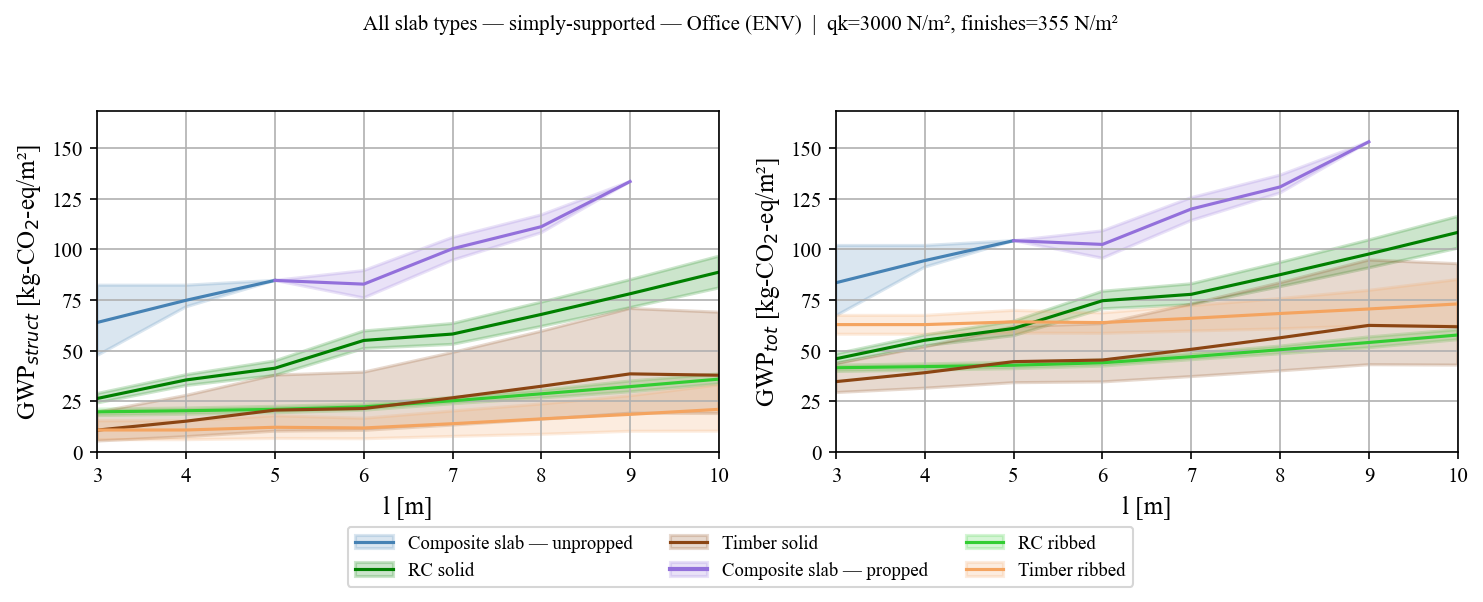
\includegraphics[width=\textwidth]{figures/office/C20/plot_office_1span_ENV_gwpC20.png}
\caption{Office single span, C20/25-only re-run: structural and total GWP versus span for all five floor systems.}
\label{fig:c20_gwp}
\end{figure}
 
\begin{table}[h!]
\centering
\caption{Office single-span composite optimum: baseline (C25/30/C30/37 permitted) versus the C20/25-only re-run.}
\label{tab:c20_sensitivity}
\small
\begin{tabular}{c c c c c c c}
\hline
& \multicolumn{2}{c}{Baseline} & \multicolumn{2}{c}{C20/25 only} & & \\
$L$ [m] & $h$ [mm] & GWP$_{\text{tot}}$ & $h$ [mm] & GWP$_{\text{tot}}$ & $\Delta$GWP & Governing check \\
\hline
3 & 198 & 67.6 & 198 & 67.3 & $-0.3$ & Fire D1 (unchanged) \\
4 & 357 & 91.8 & 357 & 91.3 & $-0.5$ & Fire D4 (unchanged) \\
5 & 279 & 104.7 & 279 & 104.3 & $-0.4$ & Fire D4 (unchanged) \\
6 & 365 & 95.4 & 369 & 95.6 & $+0.2$ & SLS deflection (unchanged) \\
7 & 441 & 114.0 & 447 & 114.3 & $+0.3$ & SLS deflection (unchanged) \\
8 & 504 & 127.4 & 512 & 127.8 & $+0.4$ & SLS deflection (unchanged) \\
9 & 455 & 152.5 & 464 & 153.1 & $+0.6$ & SLS deflection (unchanged) \\
\hline
\end{tabular}
\end{table}
 
The result is that permitting C20/25 changes the single-span composite GWP by less than 0.6\,kg\,CO\textsubscript{2}eq/m\textsuperscript{2} at every span---under 1\,\% of the total---and the governing check is unchanged at every point. More importantly, the sign of the change reverses across the span range, which explains why the intuition that ``the lowest-GWP grade would always be chosen'' does not hold. At the short spans (3--5\,m) the section is governed by the fire thermal-insulation (D1) and minimum-effective-thickness (D4) checks, both of which are independent of concrete grade; the depth is therefore fixed by fire, the same deck and depth are selected, and the only effect of the weaker grade is its lower GWP intensity, giving a marginal \emph{saving} of 0.3--0.5\,kg\,CO\textsubscript{2}eq/m\textsuperscript{2}. From 6\,m upward the section is governed by SLS deflection; here C20/25's lower elastic modulus ($E_{cm}$) reduces the composite stiffness, so the optimiser must add 4--9\,mm of depth to the same deck profile to satisfy the $L/300$ limit, and the additional concrete slightly outweighs the lower per-kilogram intensity, giving a net penalty of 0.2--0.6\,kg\,CO\textsubscript{2}eq/m\textsuperscript{2}. The lowest-GWP grade is therefore selected only where the design is grade-independent; wherever stiffness governs---most of the practical range---a weaker grade is mildly counterproductive.
 
Two conclusions follow. First, the practice-based restriction to C25/30 and C30/37 does not materially affect the reported results: the largest single-span effect of permitting C20/25 is a 0.6\,kg\,CO\textsubscript{2}eq/m\textsuperscript{2} change, negligible against the 1.4--1.8$\times$ gap between the composite slab and the RC flat baseline (Section~\ref{sec:disc_literature}), so none of the comparative rankings or conclusions of Chapter~\ref{fourthchapter} are altered. Second, and perhaps more usefully, the exercise confirms that composite slab GWP is not reduced by specifying a lower-strength concrete: because the design is stiffness-governed over most of the range, any saving from a weaker grade is recovered---or exceeded---by the compensating increase in depth. The restriction is therefore justified not only on practice grounds but also because relaxing it would, if anything, slightly worsen the composite GWP at some spans.

%==============================================================================
\subsection{Swiss market context}
\label{sec:disc_swiss}
%==============================================================================
The deck products in the optimisation database --- Tata Steel ComFlor and Kingspan Multideck --- are manufactured in the United Kingdom and marketed principally in the UK and Irish markets. \cite{RefWorks:2017comflor} describe the ComFlor range as manufactured in the UK and \enquote{readily available} within Europe, while Kingspan Multideck is likewise produced at a single facility in North Yorkshire \citep{RefWorks:kingspan2026multideck}. Neither manufacturer operates a Swiss production or distribution entity.

Profiled steel composite decking is an established product category in Switzerland. Montana Bausysteme AG, a Swiss company of the Tata Steel Europe group since 1964, manufactures and supplies the Holorib\textsuperscript{\textregistered} and SuperHolorib\textsuperscript{\textregistered} composite floor deck ranges from its Swiss facility \citep{Montana_Holorib}. These are re-entrant dovetail profiles designed for composite slab construction per EN~1994-1-1, approved for static and dynamic loading by Swiss building authorities, and have been used in industrial halls, office buildings, multi-storey car parks, and residential construction \citep{Montana_Holorib}. The existence of this Tata Steel-affiliated supply chain suggests that composite steel decking is available in the Swiss market; the specific profiles in the optimisation database (ComFlor~46 to ComFlor~225, Multideck~50 to Multideck~146) are however distinct products from the Montana range and would require independent confirmation of availability before the optimisation results could be applied directly.

ArcelorMittal operates a Swiss-facing market entity that actively markets the Cofraplus\textsuperscript{\textregistered}, Cofrastra\textsuperscript{\textregistered}, and Cofradal\textsuperscript{\textregistered} composite floor deck ranges to Swiss specifiers \citep{AM_schweiz_cofraplus,AM_schweiz_cofradal}. As noted in Section~\ref{sec:epd_deck_assumptions}, ArcelorMittal products were excluded from the main optimisation runs on grounds of EPD inconsistency, not market availability: the single flat-rate area declaration (18.0\,kg\,CO$_2$eq/m$^2$ across all products) is physically implausible and would introduce a systematic bias in favour of the deep-profile configurations where the underestimation is most severe. The availability of ArcelorMittal products in Switzerland therefore reinforces the conclusion that the composite floor slab concept is applicable to Swiss practice, even if the specific GWP results reported here cannot be directly attributed to ArcelorMittal products.

%==============================================================================
\subsection{Further work}
\label{sec:disc_future}
%==============================================================================
Several extensions follow directly from the limitations above.

\paragraph{Cost analysis.} The most significant extension is a cost comparison alongside the GWP comparison. Because the systems differ greatly in construction method---composite construction trades higher material carbon for faster erection and reduced formwork---a cost and programme analysis would test whether the GWP penalty of composite construction is offset by economic and time savings.

\paragraph{Low-carbon steel.}
The composite slab GWP is dominated by the profiled steel deck, which accounts for roughly 40--55\,\% of \gwpstruct{} across the office span range examined (Section~\ref{sec:res_office_breakdown}). Recycled-content or electric-arc-furnace ("green") steel, with a markedly lower GWP intensity than the values used here, would reduce the composite GWP substantially and could narrow the gap to the RC systems.

The baseline EPD intensities used in this study are those of the Tata Steel ComFlor product range (2.79--3.09\,kg\,CO$_2$eq/kg, declared per m$^2$ of profile) and the Kingspan Multideck range (2.50\,kg\,CO$_2$eq/kg, declared per tonne). ArcelorMittal Building Solutions has published an Environmental Product Declaration for deck profiles produced from XCarb\textsuperscript{\textregistered} recycled and renewably produced steel \citep{RefWorks:RefID:121-2025deck}. The declared GWP (A1--A3, total) for a standard deck configuration with a self-weight of 8.89\,kg/m$^2$ is 8.47\,kg\,CO$_2$eq/m$^2$, equivalent to an intensity of 0.95\,kg\,CO$_2$eq/kg --- a reduction of approximately 67\,\% relative to the standard ArcelorMittal deck profile \citep{RefWorks:RefID:115-peters2022epdamc20210146cbb2en} value of $\approx$2.92\,kg\,CO$_2$eq/kg.

To estimate the effect on the optimised office results, the deck EPD intensity in each optimal single-span solution was replaced with the XCarb\textsuperscript{\textregistered} value of 0.95\,kg\,CO$_2$eq/kg while holding all other components (concrete, mesh, trough bars) constant. The results are summarised in Table~\ref{tab:xcarb_sensitivity}. Across the full span range, replacing the conventional deck with a
XCarb\textsuperscript{\textregistered}-equivalent product reduces the structural GWP by 20--42\,\%, with an average reduction of approximately 34\,\%.

\begin{table}[htbp]
  \centering
  \caption{Sensitivity of single-span office to substitution of a low-carbon (XCarb\textsuperscript{\textregistered}-equivalent) deck EPD intensity (0.95\,kg\,CO$_2$eq/kg) for the conventional Tata Steel / Kingspan baseline. All values in kg\,CO$_2$eq/m$^2$.}
  \label{tab:xcarb_sensitivity}
  \small
  \begin{tabular}{ccllrrrc}
    \toprule
    Span & Governing & \multicolumn{2}{c}{GWP$_{struct}$} & \multicolumn{2}{c}{Deck GWP} & \multirow{2}{*}{\shortstack{Reduction\\(kg\,CO$_2$eq/m$^2$)}} & \multirow{2}{*}{\shortstack{Reduction\\(\%)}} \\
    \cmidrule(lr){3-4}\cmidrule(lr){5-6}
    (m) & deck & Baseline & XCarb & Baseline & XCarb \\
    \midrule
    3 & Multideck~60~0.9   & 42.2 & 27.7 & 23.4 &  8.9 & 14.5 & 34.3 \\
    4 & Multideck~80~1.0   & 52.7 & 34.9 & 28.8 & 11.2 & 17.8 & 33.8 \\
    5 & ComFlor~60~0.9     & 64.2 & 44.5 & 29.2 &  9.5 & 19.8 & 30.7 \\
    6 & ComFlor~210        & 75.8 & 44.1 & 46.9 & 15.3 & 31.7 & 41.8 \\
    7 & ComFlor~225        & 94.4 & 61.3 & 49.1 & 16.0 & 33.2 & 35.1 \\
    8 & ComFlor~225        &107.8 & 74.6 & 49.1 & 16.0 & 33.2 & 30.8 \\
    9 & Multideck~146~1.5  &132.9 & 95.3 & 60.8 & 19.8 & 37.7 & 28.3 \\
    \bottomrule
  \end{tabular}
\end{table}

Section~\ref{sec:res_office_breakdown} shows that the optimal single-span RC flat slab (solid) occupies a range of approximately 70--150\,kg\,CO$_2$eq/m$^2$ over the same span range. The XCarb\textsuperscript{\textregistered} values of 28--95\,kg\,CO$_2$eq/m$^2$ indicate that a low-carbon supply chain could bring the composite slab GWP below the RC flat-slab benchmark across virtually the entire span range studied, entirely through a decarbonised steel supply chain and with no structural redesign. This sensitivity highlights the particular responsiveness of the composite system to supply-chain decarbonisation: because the deck dominates the GWP budget, the composite slab is the floor system most immediately affected by --- and most likely to benefit from --- the transition to EAF-route low-carbon steel.

Direct numerical comparison of GWP values across the two standard versions is not formally valid because the impact characterisation factors and system boundaries differ between versions. The XCarb\textsuperscript{\textregistered} EPD covers ArcelorMittal decks, which are not the same products as the Tata Steel ComFlor or Kingspan Multideck profiles optimised in this study; the sensitivity should therefore be read as illustrative of the effect of an EAF-route low-carbon steel supply chain, rather than as a statement that the XCarb\textsuperscript{\textregistered} product specifically achieves the stated structural performance. Subject to these caveats, the calculation represents a credible order-of-magnitude estimate of the carbon savings achievable through supply-chain decarbonisation of the steel deck, and confirms that low-carbon steel is the dominant lever for reducing the embodied carbon of the composite floor system.

\paragraph{End-of-life and module D.} Extending the LCA boundary to include end-of-life recovery (module D) would credit the recyclability and potential demountability of the steel components, and is expected to favour the composite and steel-containing systems relative to the cradle-to-gate comparison used here.

\paragraph{Continuous-span extension of all systems.} Extending the RC ribbed and timber systems to continuous spans would allow a fully consistent cross-system comparison in the continuous configurations, rather than the single-span baselines used at present.

\paragraph{System boundary: slab level only.} The comparison is conducted at the floor-slab level and excludes the supporting structural system. Composite slabs are inherently coupled to a steel frame:  primary and secondary steel beams, which carry substantial embodied carbon, are required and are not present in an equivalent RC flat-slab system. At the full-building scale this represents a material carbon cost not captured in the present comparison, and is expected to widen the GWP gap between composite and RC construction. In the opposing direction, a steel-framed building is substantially lighter than its RC equivalent --- a reduction in superstructure --- which reduces foundation loads and consequently the volume of concrete and reinforcement in the foundations. In ground conditions where piling is substantial, this saving can be material. The net effect at the full-building scale is therefore ambiguous without a complete structural system assessment, and the slab-level comparison presented here should be interpreted accordingly.

\paragraph{Optimiser treatment of propping and shear connection.} Two refinements to the optimisation itself would improve the realism of the comparison. First, the current routine treats propping as a binary fallback, selecting an unpropped section wherever one is feasible and resorting to propping only when no unpropped solution exists, even though propping was shown to yield a lower-GWP section at several spans (Section~\ref{sec:res_office_gov}). Introducing an explicit penalty on propped construction---representing its programme and cost impact---would allow the optimiser to trade the GWP saving of a propped section against its construction-stage disadvantage on a consistent basis, rather than suppressing propped solutions outright. Second, shear connection is presently fixed at the embossment-and-friction shear bond, with end anchorage omitted (Section~\ref{sec:assumptions}). Treating the provision of shear connectors as an additional design variable would let the optimiser thin the deck or reduce its depth where the added connector capacity permits, potentially lowering the overall GWP; the connector GWP would need to be added to the objective so that the trade-off is captured honestly.
    \section{Conclusion}
\label{sixthchapter}
%===============================================================
\subsection{Introduction}
%===============================================================

    % ... Add more chapters as needed

    % Bibliography
    \pagestyle{plain}
    % Changes the page style to 'plain' for the bibliography section, typically removing headers and using simple footers.

    \clearpage

    %\printbibliography
    % Prints the bibliography based on the entries in 'references.bib' and the settings defined in the preamble.
    \bibliography{bib/references}
    \bibliographystyle{apalike}
    \nocite{*}

    \addcontentsline{toc}{section}{References}
    % Adds an entry titled "References" to the table of contents.

    \clearpage

    % Appendices
    \appendix
\section{Appendix}
\label{appendix}
%===============================================================
\subsection{AI Use Declaration}
To ensure transparency and uphold academic integrity, the following table outlines the artificial intelligence (AI) tools utilized during the preparation of this report. This declaration aligns with ETH Zurich's guidelines on the responsible use of AI in scientific writing.

documentation?
other figures not used?
code?

\subsection{Decking product database}
\label{app:decking_db}
The tables below list all profiled steel decking products included in the optimisation database, with geometry and section properties (Table~\ref{tab:deck_db_geom}) and structural resistances with EPD data (Table~\ref{tab:deck_db_resist}). Values are sourced from manufacturer technical manuals and EPD documents as referenced in Section~\ref{sec:database}.

% Auto-generated by generate_decking_table.py — do not edit manually.
% Re-run the script if the database changes.

\begingroup
\scriptsize
\setlength{\tabcolsep}{4pt}
\renewcommand{\arraystretch}{1.15}

\begin{longtable}{@{}llcrrrrrrrrr@{}}
\caption{Decking product database --- geometry and section properties}
\label{tab:deck_db_geom}\\
\toprule
\textbf{Product} & \textbf{Mfr.} & \textbf{Type} & $h_p$ & $t$ & $l_1$ & $l_2$ & $l_3$ & $w$ & $A_p$ & $A_{p,e}$ & $I_p$ \\
 & & & [mm] & [mm] & [mm] & [mm] & [mm] & [kg/m\textsuperscript{2}] & [mm\textsuperscript{2}/m] & [mm\textsuperscript{2}/m] & [cm\textsuperscript{4}/m] \\
\midrule
\endfirsthead
\toprule
\textbf{Product} & \textbf{Mfr.} & \textbf{Type} & $h_p$ & $t$ & $l_1$ & $l_2$ & $l_3$ & $w$ & $A_p$ & $A_{p,e}$ & $I_p$ \\
\midrule
\endhead
\midrule
\multicolumn{12}{r}{\textit{Continued on next page}} \\
\endfoot
\bottomrule
\endlastfoot
Cofrastra 40 0.75 & AM & Reentrant & 40 & 0.8 & 104 & 124 & 46 & 9.80 & 1183 & 1013 & 17.58 \\
Cofrastra 40 0.88 & AM & Reentrant & 40 & 0.9 & 104 & 124 & 46 & 11.50 & 1400 & 1099 & 22.23 \\
Cofrastra 40 1.0 & AM & Reentrant & 40 & 1.0 & 104 & 124 & 46 & 13.10 & 1600 & 1370 & 25.41 \\
Cofrastra 56S 0.75 & AM & Reentrant & 56 & 0.8 & 110 & 137 & 40 & 11.60 & 1402 & 1262 & 47.10 \\
Cofrastra 56S 0.88 & AM & Reentrant & 56 & 0.9 & 110 & 137 & 40 & 13.60 & 1659 & 1493 & 61.30 \\
Cofrastra 56S 1.0 & AM & Reentrant & 56 & 1.0 & 110 & 137 & 40 & 15.50 & 1896 & 1706 & 74.40 \\
Cofrastra 56S 1.13 & AM & Reentrant & 56 & 1.1 & 110 & 137 & 40 & 17.50 & 2153 & 1938 & 84.40 \\
Cofrastra 56S 1.25 & AM & Reentrant & 56 & 1.2 & 110 & 137 & 40 & 19.40 & 2390 & 2151 & 93.60 \\
Cofraplus 60 0.75 & AM & Trapezoidal & 60 & 0.8 & 101 & 62 & 106 & 8.53 & 1029 & 902 & 44.37 \\
Cofrastra 60 0.88 & AM & Trapezoidal & 60 & 0.9 & 101 & 62 & 106 & 10.00 & 1217 & 1067 & 52.64 \\
Cofrastra 60 1.0 & AM & Trapezoidal & 60 & 1.0 & 101 & 62 & 106 & 11.37 & 1391 & 1220 & 60.08 \\
Cofrastra 60 1.25 & AM & Trapezoidal & 60 & 1.2 & 101 & 62 & 106 & 14.22 & 1797 & 1537 & 75.10 \\
Cofrastra 70 0.75 & AM & Trapezoidal & 70 & 0.8 & 113 & 87 & 70 & 10.05 & 1219 & 998 & 22.05 \\
Cofrastra 70 0.88 & AM & Trapezoidal & 70 & 0.9 & 113 & 87 & 70 & 11.80 & 1442 & 1181 & 25.99 \\
Cofrastra 70 1.0 & AM & Trapezoidal & 70 & 1.0 & 113 & 87 & 70 & 13.40 & 1648 & 1350 & 29.62 \\
Cofraplus 80 0.88 & AM & Reentrant & 80 & 0.9 & 153 & 87 & 117 & 10.66 & 1296 & 1182 & 141.58 \\
Cofrastra 80 1.0 & AM & Reentrant & 80 & 1.0 & 153 & 87 & 117 & 12.11 & 1481 & 1351 & 158.79 \\
Cofrastra 80 1.13 & AM & Reentrant & 80 & 1.1 & 153 & 87 & 117 & 13.69 & 1682 & 1534 & 177.43 \\
Cofrastra 80 1.25 & AM & Reentrant & 80 & 1.2 & 153 & 87 & 117 & 15.14 & 1867 & 1702 & 194.64 \\
Cofraplus 220 1.13 & AM & Trapezoidal & 220 & 1.1 & 84 & 83 & 666 & 15.14 & 1817 & 908 & 926.00 \\
Cofraplus 220 1.25 & AM & Trapezoidal & 220 & 1.2 & 84 & 83 & 666 & 16.75 & 2017 & 1008 & 1063.00 \\
Multideck 50 0.85 & KSP & Reentrant & 50 & 0.8 & 110 & 135 & 40 & 11.42 & 1418 & 1276 & 56.58 \\
Multideck 50 0.9 & KSP & Reentrant & 50 & 0.9 & 110 & 135 & 40 & 12.89 & 1605 & 1444 & 66.15 \\
Multideck 50 1.0 & KSP & Reentrant & 50 & 1.0 & 110 & 135 & 40 & 14.36 & 1792 & 1613 & 75.90 \\
Multideck 50 1.1 & KSP & Reentrant & 50 & 1.1 & 110 & 135 & 40 & 15.83 & 1979 & 1781 & 83.99 \\
Multideck 50 1.2 & KSP & Reentrant & 50 & 1.2 & 110 & 135 & 40 & 17.29 & 2165 & 1948 & 92.16 \\
Multideck 60 0.9 & KSP & Trapezoidal & 60 & 0.9 & 190 & 119 & 142 & 9.34 & 1138 & 1024 & 81.00 \\
Multideck 60 1.0 & KSP & Trapezoidal & 60 & 1.0 & 190 & 119 & 142 & 10.37 & 1270 & 1143 & 91.83 \\
Multideck 60 1.1 & KSP & Trapezoidal & 60 & 1.1 & 190 & 119 & 142 & 11.41 & 1402 & 1262 & 102.70 \\
Multideck 60 1.2 & KSP & Trapezoidal & 60 & 1.2 & 190 & 119 & 142 & 12.45 & 1535 & 1381 & 112.30 \\
Multideck 80 1.0 & KSP & Trapezoidal & 80 & 1.0 & 169 & 102 & 131 & 11.49 & 1413 & 1272 & 171.30 \\
Multideck 80 1.1 & KSP & Trapezoidal & 80 & 1.1 & 169 & 102 & 131 & 12.64 & 1560 & 1404 & 190.60 \\
Multideck 80 1.2 & KSP & Trapezoidal & 80 & 1.2 & 169 & 102 & 131 & 13.83 & 1705 & 1535 & 208.60 \\
Multideck 146 1.2 & KSP & Trapezoidal & 160 & 1.2 & 134 & 61 & 131 & 19.40 & 2400 & 2160 & 836.00 \\
Multideck 146 1.5 & KSP & Trapezoidal & 160 & 1.5 & 134 & 61 & 131 & 24.30 & 3020 & 2718 & 1080.00 \\
ComFlor 46 0.9 & Tata & Trapezoidal & 46 & 0.9 & 158 & 105 & 67 & 9.17 & 1137 & 848 & 41.50 \\
ComFlor 46 1.2 & Tata & Trapezoidal & 46 & 1.2 & 158 & 105 & 67 & 13.25 & 1534 & 1130 & 53.00 \\
ComFlor 51 0.9 & Tata & Reentrant & 51 & 0.9 & 110 & 135 & 40 & 13.25 & 1578 & 1494 & 60.44 \\
ComFlor 51 1.0 & Tata & Reentrant & 51 & 1.0 & 110 & 135 & 40 & 14.27 & 1762 & 1680 & 67.09 \\
ComFlor 51 1.2 & Tata & Reentrant & 51 & 1.2 & 110 & 135 & 40 & 17.33 & 2137 & 2044 & 82.60 \\
ComFlor 60 0.9 & Tata & Trapezoidal & 60 & 0.9 & 170 & 120 & 130 & 10.19 & 1276 & 1176 & 92.77 \\
ComFlor 60 1.0 & Tata & Trapezoidal & 60 & 1.0 & 170 & 120 & 130 & 11.21 & 1424 & 1314 & 106.15 \\
ComFlor 60 1.2 & Tata & Trapezoidal & 60 & 1.2 & 170 & 120 & 130 & 14.27 & 1721 & 1576 & 132.91 \\
ComFlor 80 0.9 & Tata & Trapezoidal & 80 & 0.9 & 150 & 120 & 150 & 11.21 & 1382 & 1244 & 165.42 \\
ComFlor 80 1.2 & Tata & Trapezoidal & 80 & 1.2 & 150 & 120 & 150 & 15.29 & 1864 & 1678 & 213.13 \\
ComFlor 210 & Tata & Trapezoidal & 210 & 1.2 & 178 & 54 & 422 & 16.31 & 2009 & 787 & 816.00 \\
ComFlor 225 & Tata & Trapezoidal & 225 & 1.2 & 200 & 102 & 400 & 17.33 & 2108 & 1353 & 1089.80 \\
\end{longtable}

\begin{longtable}{@{}llrrrrrrll@{}}
\caption{Decking product database --- resistances, shear parameters, and EPD data}
\label{tab:deck_db_resist}\\
\toprule
\textbf{Product} & \textbf{Mfr.} & $M_{c,Rd}$ & $M_{t,Rd}$ & $m_p$ & $k_p$ & $\tau_{u,Rk}$ & GWP & Unit \\
 & & [kNm/m] & [kNm/m] & [kN/m\textsuperscript{2}] & [kN/m\textsuperscript{2}] & [N/mm\textsuperscript{2}] & [kg\,CO\textsubscript{2}/unit] & \\
\midrule
\endfirsthead
\toprule
\textbf{Product} & \textbf{Mfr.} & $M_{c,Rd}$ & $M_{t,Rd}$ & $m_p$ & $k_p$ & $\tau_{u,Rk}$ & GWP & Unit \\
\midrule
\endhead
\midrule
\multicolumn{9}{r}{\textit{Continued on next page}} \\
\endfoot
\bottomrule
\endlastfoot
Cofrastra 40 0.75 & AM & 3.40 & --- & --- & --- & 0.2900 & 18.012 & m2 \\
Cofrastra 40 0.88 & AM & 4.45 & --- & --- & --- & 0.2900 & 18.012 & m2 \\
Cofrastra 40 1.0 & AM & 5.08 & --- & --- & --- & 0.2900 & 18.012 & m2 \\
Cofrastra 56S 0.75 & AM & 4.27 & --- & --- & --- & 0.3400 & 18.012 & m2 \\
Cofrastra 56S 0.88 & AM & 5.97 & --- & --- & --- & 0.3400 & 18.012 & m2 \\
Cofrastra 56S 1.0 & AM & 7.54 & --- & --- & --- & 0.3400 & 18.012 & m2 \\
Cofrastra 56S 1.13 & AM & 9.69 & --- & --- & --- & 0.3400 & 18.012 & m2 \\
Cofrastra 56S 1.25 & AM & 11.67 & --- & --- & --- & 0.3400 & 18.012 & m2 \\
Cofraplus 60 0.75 & AM & 4.21 & --- & --- & --- & 0.1000 & 18.012 & m2 \\
Cofrastra 60 0.88 & AM & 5.39 & --- & --- & --- & 0.1000 & 18.012 & m2 \\
Cofrastra 60 1.0 & AM & 6.59 & --- & --- & --- & 0.1000 & 18.012 & m2 \\
Cofrastra 60 1.25 & AM & 8.24 & --- & --- & --- & 0.1000 & 18.012 & m2 \\
Cofrastra 70 0.75 & AM & 7.65 & --- & --- & --- & 0.1400 & 18.012 & m2 \\
Cofrastra 70 0.88 & AM & 9.81 & --- & --- & --- & 0.1400 & 18.012 & m2 \\
Cofrastra 70 1.0 & AM & 12.02 & --- & --- & --- & 0.1400 & 18.012 & m2 \\
Cofraplus 80 0.88 & AM & 12.69 & --- & --- & --- & 0.2300 & 18.012 & m2 \\
Cofrastra 80 1.0 & AM & 15.03 & --- & --- & --- & 0.2300 & 18.012 & m2 \\
Cofrastra 80 1.13 & AM & 17.72 & --- & --- & --- & 0.2300 & 18.012 & m2 \\
Cofrastra 80 1.25 & AM & 20.33 & --- & --- & --- & 0.2300 & 18.012 & m2 \\
Cofraplus 220 1.13 & AM & 20.27 & --- & 214.8 & 0.0284 & --- & 18.012 & m2 \\
Cofraplus 220 1.25 & AM & 23.27 & --- & 214.8 & 0.0284 & --- & 18.012 & m2 \\
Multideck 50 0.85 & KSP & 6.47 & 6.30 & 220.7 & 0.1790 & --- & 2503.803 & ton \\
Multideck 50 0.9 & KSP & 7.72 & 7.22 & 220.7 & 0.1790 & --- & 2503.803 & ton \\
Multideck 50 1.0 & KSP & 8.97 & 7.99 & 220.7 & 0.1790 & --- & 2503.803 & ton \\
Multideck 50 1.1 & KSP & 10.17 & 8.82 & 220.7 & 0.1790 & --- & 2503.803 & ton \\
Multideck 50 1.2 & KSP & 11.31 & 9.55 & 220.7 & 0.1790 & --- & 2503.803 & ton \\
Multideck 60 0.9 & KSP & 7.09 & 6.95 & 136.9 & 0.0320 & --- & 2503.803 & ton \\
Multideck 60 1.0 & KSP & 8.41 & 8.06 & 136.9 & 0.0320 & --- & 2503.803 & ton \\
Multideck 60 1.1 & KSP & 9.72 & 9.15 & 136.9 & 0.0320 & --- & 2503.803 & ton \\
Multideck 60 1.2 & KSP & 11.01 & 10.22 & 136.9 & 0.0320 & --- & 2503.803 & ton \\
Multideck 80 1.0 & KSP & 12.62 & 9.94 & 135.0 & 0.0320 & --- & 2503.803 & ton \\
Multideck 80 1.1 & KSP & 14.39 & 11.33 & 135.0 & 0.0320 & --- & 2503.803 & ton \\
Multideck 80 1.2 & KSP & 16.42 & 12.73 & 135.0 & 0.0320 & --- & 2503.803 & ton \\
Multideck 146 1.2 & KSP & 32.04 & --- & 154.1 & 0.0780 & --- & 2503.803 & ton \\
Multideck 146 1.5 & KSP & 42.30 & --- & 297.2 & 0.0310 & --- & 2503.803 & ton \\
ComFlor 46 0.9 & Tata & 4.63 & 4.67 & 41.7 & 0.0730 & --- & 27.624 & m2 \\
ComFlor 46 1.2 & Tata & 5.99 & 6.23 & 41.7 & 0.0730 & --- & 36.930 & m2 \\
ComFlor 51 0.9 & Tata & 5.70 & 6.78 & --- & --- & 0.2700 & 37.514 & m2 \\
ComFlor 51 1.0 & Tata & 6.78 & 8.17 & --- & --- & 0.2700 & 41.544 & m2 \\
ComFlor 51 1.2 & Tata & 8.94 & 10.96 & --- & --- & 0.2700 & 49.618 & m2 \\
ComFlor 60 0.9 & Tata & 9.30 & 7.50 & --- & --- & 0.2600 & 29.219 & m2 \\
ComFlor 60 1.0 & Tata & 11.27 & 9.36 & --- & --- & 0.2600 & 34.388 & m2 \\
ComFlor 60 1.2 & Tata & 15.21 & 13.07 & --- & --- & 0.2600 & 41.104 & m2 \\
ComFlor 80 0.9 & Tata & 10.76 & 8.68 & --- & --- & 0.2100 & 34.686 & m2 \\
ComFlor 80 1.2 & Tata & 18.49 & 14.59 & --- & --- & 0.2100 & 44.511 & m2 \\
ComFlor 210 & Tata & 23.20 & 23.20 & 221.0 & 0.0376 & --- & 46.949 & m2 \\
ComFlor 225 & Tata & 31.66 & 23.58 & 214.8 & 0.0284 & --- & 49.075 & m2 \\
\end{longtable}
\endgroup
%===============================================================
\subsection{Full-floor vibration check: worked example}
\label{app:vibration}
%===============================================================
This appendix presents a complete bay-level vibration check for a representative office floor, following the full SCI~P354 method \citep{RefWorks:hicks2009p354}. It is included to demonstrate the full procedure that the slab-only screening check of Section~\ref{sec:vibration_method} approximates, and to quantify the extent to which the complete floor frequency --- with the slab supported on flexible beams --- falls below the slab-alone value. The calculation is implemented in \texttt{full\_vibration\_check.py}.

\subsubsection*{Bay geometry and inputs}
The worked example uses a representative office bay. The inputs that the slab-only optimisation cannot define --- and which the full check requires --- are stated explicitly below.
\todo[inline]{Populate from full\_vibration\_check.py for the chosen representative bay. Fill in: secondary beam span, primary beam span, bay width, secondary/primary beam sections, slab depth and deck, concrete grade, damping ratio $\zeta$, and the design walking parameters.}

\begin{table}[h!]
\small
\centering
\caption{Bay geometry and design inputs for the worked vibration example.}
\label{tab:vib_example_inputs}
\begin{tabular}{lll}
\toprule
Parameter & Symbol & Value \\
\midrule
Secondary beam span        & $L_s$        & \todo{fill}\,m \\
Primary beam span          & $L_p$        & \todo{fill}\,m \\
Bay width                  & $w_\mathrm{bay}$ & \todo{fill}\,m \\
Secondary beam section     & ---          & \todo{fill} \\
Primary beam section       & ---          & \todo{fill} \\
Slab depth / deck          & $h$          & \todo{fill}\,mm / \todo{fill} \\
Concrete grade             & ---          & \todo{fill} \\
Floor mass (perm.\ + $0.1Q_k$) & $m$      & \todo{fill}\,kg/m\textsuperscript{2} \\
Damping ratio              & $\zeta$      & \todo{fill} (SCI~P354 Table~4.1) \\
\bottomrule
\end{tabular}
\end{table}

\subsubsection*{Step 1 --- Component frequencies}
The natural frequency of each component (slab, secondary beam, primary beam) is computed from its self-weight deflection $\delta$ under the vibrating mass using $f = 18/\sqrt{\delta_\mathrm{mm}}$ (SCI~P354 Eq.~4).
\todo[inline]{Report $\delta$ and $f$ for the slab, secondary beam, and primary beam. Note the slab value here should match the slab-only screening value of Section~\ref{sec:vibration_method} for the same span.}

\subsubsection*{Step 2 --- Combined floor frequency}
The component frequencies are combined using Dunkerley's approximation to give the fundamental frequency of the floor system:
\begin{equation}
    \frac{1}{f_0^2} = \frac{1}{f_\mathrm{slab}^2} + \frac{1}{f_\mathrm{sec}^2} + \frac{1}{f_\mathrm{prim}^2}
    \label{eq:dunkerley}
\end{equation}
\todo[inline]{Report the combined $f_0$ and compare it explicitly with the slab-alone frequency, stating the percentage reduction. This is the key quantitative point: the full-floor frequency is lower than the slab-alone screening value.}

\subsubsection*{Step 3 --- Modal mass and response factor}
The floor is classified as low- or high-frequency from $f_0$, the effective modal mass mobilised by walking is estimated, and the root-mean-square acceleration response is computed and expressed as a response factor $R$ relative to the BS~6472 base curve.
\todo[inline]{Report: classification (low/high frequency), modal mass, RMS acceleration $a_\mathrm{rms}$, and the resulting response factor $R$. State the acceptance limit used (e.g.\ $R \le 8$ for general offices, SCI~P354) and whether the bay passes.}

\subsubsection*{Discussion of the example}
\todo[inline]{Close with 2--3 sentences: (1) whether the representative bay passes the full check; (2) how far the full-floor frequency sits below the slab-alone screening value, confirming the screening check is conservative-but-necessary as described in Section~\ref{sec:vibration_method}; (3) the implication for the optimisation results --- i.e.\ that at long office spans the full check would likely require a deeper section than the optimisation selects, as discussed in Section~\ref{sec:assumptions}.}

    % Includes the content of 'appendix.tex' which should contain any supplementary material or appendices.

\end{document}
